% =============================================================================
% O LIVRO — escrito à mão, em português do Brasil.
%
% Esta é a raiz do artefato central. O que vive aqui é texto; número medido vem
% de livro/numeros.tex e figura vem de livro/figuras/ (as duas geradas por
% lab/executar.py), e a bibliografia vem de livro/fontes.tex (gerada por
% lab/fontes.py). Arquivo gerado não se edita à mão.
%
% Estrutura (AGENTS.md §6): raiz, quatro voltas, travessia, dois andares e fecho --- as seis
% partes impressas, na ordem em que o livro as percorre.
% Nenhum capítulo entra sem o fracasso concreto que o abre, com número na mão.
% =============================================================================
\documentclass[11pt,a4paper]{book}

\usepackage[utf8]{inputenc}
\usepackage[T1]{fontenc}
\usepackage{lmodern}   % herdado do arquivo: microtype exige fonte escalável
\usepackage{amsmath,amssymb,amsthm,mathtools}
\usepackage{graphicx}
\usepackage{geometry}
\geometry{margin=1.15in}
\usepackage{microtype}
\usepackage{bm}
\usepackage{enumitem}
\usepackage{xcolor}
\usepackage{hyperref}
\hypersetup{colorlinks=true, linkcolor=blue!70!black,
            citecolor=green!50!black, urlcolor=blue!80!black}
\usepackage[capitalise,noabbrev]{cleveref}
\usepackage{url}

% Nomes em português. A distribuição local não traz o pacote de idioma do babel
% (herdado do arquivo: "Unknown option 'brazilian'"), então os poucos nomes que o
% LaTeX cunha são trocados à mão.
\renewcommand{\contentsname}{Sumário}
\renewcommand{\chaptername}{Capítulo}
\renewcommand{\bibname}{Fontes}
\renewcommand{\proofname}{Prova}
% As duas que faltavam, e são as mais visíveis: a classe `book` prefixa toda
% legenda com o nome do objeto, de modo que o livro imprimia "Figure 3.2:" e
% "Table 3.1:" em cima de legenda escrita em português.
\renewcommand{\figurename}{Figura}
\renewcommand{\tablename}{Tabela}
\renewcommand{\partname}{Parte}
% A folha de parte usa o nome que a classe cunha, e sem troca ela imprimiria "Part I" no
% meio de um livro em português --- a mesma família do "Figure" e do "September". O
% `conferir_nomes` passou a exigir esta troca.
% E a data: sem babel, \today escreve "September 24, 2026" na folha de rosto.
\newcommand{\mesEmPortugues}{\ifcase\month\or janeiro\or fevereiro\or março\or abril\or maio\or junho\or julho\or agosto\or setembro\or outubro\or novembro\or dezembro\fi}

% O cleveref imprime o nome do CONTADOR, e não o do ambiente: com o contador de base chamado
% "teorema", toda referência a uma proposição saía na página como "a teorema 15.1" — com o artigo
% errado, porque quem escreve o texto escreveu "a". O nome estava declarado, o \cref existia e o
% portão passava; o que ninguém olhava era o contador. Ele agora tem o nome do tipo que o livro
% de fato referencia, e os outros ambientes continuam compartilhando o mesmo.
\newtheorem{proposicao}{Proposição}[chapter]
\newtheorem{lema}[proposicao]{Lema}
\newtheorem{teorema}[proposicao]{Teorema}
\newtheorem{corolario}[proposicao]{Corolário}
\theoremstyle{definition}
\newtheorem{definicao}[proposicao]{Definição}
\newtheorem{exemplo}[proposicao]{Exemplo}
\theoremstyle{remark}
\newtheorem{observacao}[proposicao]{Observação}

% O cleveref cunha as referências no idioma que o babel carrega; sem babel ele
% cunha em inglês, e o livro imprimia "Table 3.2" no meio de uma frase em
% português. Os nomes saem declarados um por um, e o tipo é o do contador ---
% todos os ambientes de teorema compartilham o contador `proposicao`, que é o tipo que o livro
% referencia; o portão `conferir_nomes` reprova o `\cref` cujo ambiente não seja o dono do contador.
\crefname{figure}{figura}{figuras}
\Crefname{figure}{Figura}{Figuras}
\crefname{table}{tabela}{tabelas}
\Crefname{table}{Tabela}{Tabelas}
\crefname{chapter}{capítulo}{capítulos}
\Crefname{chapter}{Capítulo}{Capítulos}
\crefname{part}{parte}{partes}
\Crefname{part}{Parte}{Partes}
\Crefname{part}{Parte}{Partes}
\crefname{section}{seção}{seções}
\Crefname{section}{Seção}{Seções}
\crefname{equation}{equação}{equações}
\Crefname{equation}{Equação}{Equações}
\crefname{teorema}{teorema}{teoremas}
\Crefname{teorema}{Teorema}{Teoremas}
\crefname{lema}{lema}{lemas}
\crefname{proposicao}{proposição}{proposições}
\Crefname{proposicao}{Proposição}{Proposições}
\crefname{corolario}{corolário}{corolários}
\crefname{definicao}{definição}{definições}
\Crefname{definicao}{Definição}{Definições}
\crefname{exemplo}{exemplo}{exemplos}
\crefname{observacao}{observação}{observações}

\newcommand{\Prob}{\mathbb{P}}
\newcommand{\E}{\mathbb{E}}

\title{A incerteza quando o mundo muda}
\author{}
\date{\mesEmPortugues\ de \the\year}

\begin{document}
\maketitle
\tableofcontents

% Números medidos, figuras e fontes: gerados, nunca editados à mão.
% GERADO POR lab/executar.py — NÃO EDITE À MÃO.
% Uma grandeza por caderno em lab/experimentos/; o livro cita, não digita.

\newcommand{\numBlocoAcimaDoDobroPct}{13,05}
\newcommand{\numBlocoDias}{60}
\newcommand{\numBlocoMediana}{2}
\newcommand{\numBlocoPior}{20}
\newcommand{\numBlocoPiorData}{20 de novembro de 2008}
\newcommand{\numBlocoPrometido}{3}
\newcommand{\numBlocosAcimaDoTetoPct}{1,951}
\newcommand{\numCorteAlternativoPct}{4,743}
\newcommand{\numCorteContaPct}{5,138}
\newcommand{\numCorteCurtoContaPct}{9,091}
\newcommand{\numCorteCurtoJanela}{21}
\newcommand{\numCorteCurtoPiorBloco}{12}
\newcommand{\numCorteCurtoTaxaPct}{9,407}
\newcommand{\numCorteJanela}{252}
\newcommand{\numCorteLongoContaPct}{4,996}
\newcommand{\numCorteLongoJanela}{1260}
\newcommand{\numCorteLongoPiorBloco}{24}
\newcommand{\numCorteLongoTaxaPct}{5,093}
\newcommand{\numCorteMedioContaPct}{6,25}
\newcommand{\numCorteMedioJanela}{63}
\newcommand{\numCorteMedioPiorBloco}{15}
\newcommand{\numCorteMedioTaxaPct}{6,612}
\newcommand{\numCortePosto}{13}
\newcommand{\numDiasMedidos}{6718}
\newcommand{\numEntregaDias}{6466}
\newcommand{\numEntregaTaxaPct}{5,135}
\newcommand{\numEntregaViolacoes}{332}
\newcommand{\numEpisodiosAcimaDoTeto}{6}
\newcommand{\numEpisodiosAnos}{2007, 2008, 2011, 2018 e 2020}
\newcommand{\numNuncaMudaMundos}{200}
\newcommand{\numNuncaMudaPiorBloco}{13}
\newcommand{\numNuncaMudaPiorMedio}{9,26}
\newcommand{\numNuncaMudaTaxaPct}{5,139 $\pm$ 0,1091}
\newcommand{\numPromessaPct}{5}
\newcommand{\numRazaoVol}{0,6749}
\newcommand{\numSerieDias}{6718}
\newcommand{\numSerieFim}{21 de setembro de 2026}
\newcommand{\numSerieInicio}{4 de janeiro de 2000}
\newcommand{\numVolHistorica}{0,1925}
\newcommand{\numVolRecente}{0,1299}


% -----------------------------------------------------------------------------
% Nota de abertura: é ela que mostra o encanamento funcionando, e fica fora das partes.
% -----------------------------------------------------------------------------
\chapter*{Como este livro mede}
\addcontentsline{toc}{chapter}{Como este livro mede}

Este livro não afirma nada sem mostrar como se mede. Cada número que aparece no
texto sai de um caderno de experimento: um caderno por medição, executável
sozinho, com os parâmetros no topo para quem quiser mexer. O caderno termina
gravando o resultado num arquivo, e cada figura sai duas vezes --- em papel, para
este livro, e em imagem, para inspeção.

O texto então não escreve o número: ele cita o comando que o laboratório gerou.
Isso parece detalhe e não é: um número digitado à mão pode divergir da medição
sem que ninguém perceba, e um número citado não pode, porque não existe em dois
lugares.

A medição de abertura serve de exemplo. Ela lê uma série longa de preços e mede a
volatilidade --- o quanto os preços costumam se mexer de um dia para o outro, na escala de tempo que
se declara --- em duas escalas de tempo: \numVolHistorica{} ao longo de todo o
histórico e \numVolRecente{} no último ano, uma razão de \numRazaoVol{} em
\numDiasMedidos{} dias úteis. A figura mostra as duas curvas que produzem esses
números.

\begin{figure}[htbp]
  \centering
  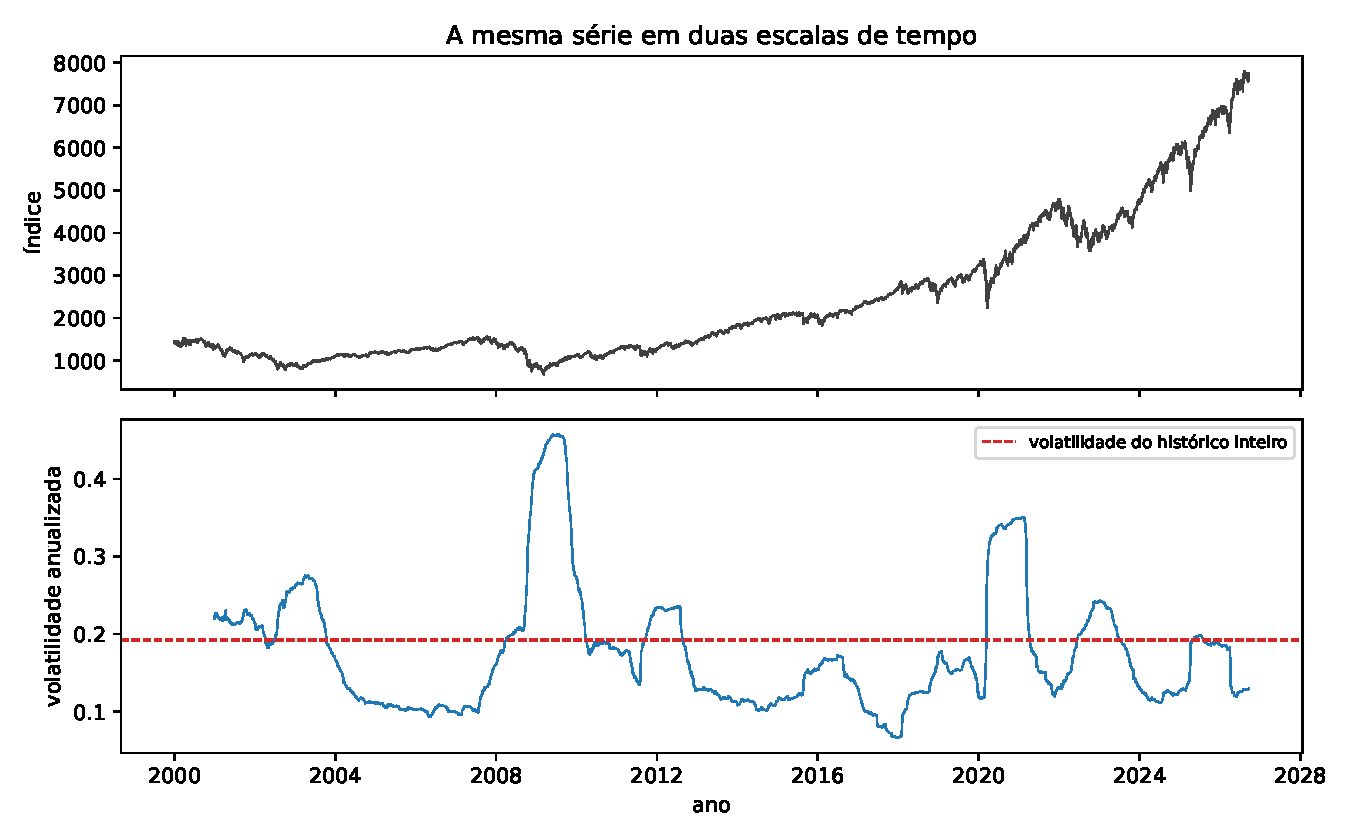
\includegraphics[width=\linewidth]{figuras/E00_pipeline_1.pdf}
  \caption{Preço e volatilidade da mesma série, em duas escalas de tempo. A linha
    tracejada é a volatilidade do histórico inteiro; a curva azul é a janela móvel
    de um ano.}
  \label{fig:encanamento}
\end{figure}

% -----------------------------------------------------------------------------
% O capítulo 1 — a raiz: o número e a barra.
% O capítulo 2 — a raiz: o que a soma guarda.
% O capítulo 3 — a raiz: a medição, o corte e o preço de fixar.
% Um arquivo por capítulo, em livro/capitulos/, nomeado pelo conceito.
% -----------------------------------------------------------------------------

\part{A raiz}

Toda conta sobre o futuro começa numa média do passado, e toda média carrega uma barra: o
tamanho do que ela se mexe sozinha. A raiz do livro mede as duas coisas na série mais simples
que existe, e mostra que o que muda no mundo não está na média.

A pergunta que sobra é a da noite: quanto se pode perder amanhã. Ela não se responde com um
centro, e sim com uma linha erguida sobre os piores dias do passado --- uma linha que tem preço,
que se mede, e que assina o que promete antes de o dado chegar.

\input{capitulos/01_o_numero_e_a_barra.tex}
% =============================================================================
% CAPÍTULO 2 — a raiz: o que a soma guarda.
%
% O fracasso que o abre, com número na mão: somar as variações diárias do índice ao longo de
% \numSomaSerieDias{} pregões entrega \numSomaVariacoesPct\% onde o índice andou
% \numSomaVariacaoRealPct\% — a metade. Num mês as duas contas quase coincidem
% (\numSomaCurtaVariacoesPct\% contra \numSomaCurtaRealPct\%), e nada avisa que a diferença cresce
% com o horizonte.
%
% Medição: lab/experimentos/E22_soma.ipynb e E44_expoente.ipynb (a inclinação da banda
% em toda escala). Figuras: figuras/E22_soma_*, E44_expoente_*.
% =============================================================================

\chapter{O que a soma guarda}
\label{cap:soma}

\section{A conta que fecha no mês e mente em vinte e seis anos}

Saber o que o índice andou parece a conta mais fácil do capítulo anterior: soma-se o que cada
dia andou, e o resultado é o que ele andou no fim. A conta tem um erro de leitura, e ele é
pequeno num mês e enorme num quarto de século.

Fizemos a conta com o dado na mão. Nos últimos \numSomaCurtaDias{} pregões, somar as variações
diárias dá \numSomaCurtaVariacoesPct\%, e o índice andou \numSomaCurtaRealPct\%: os dois
números quase coincidem, e a diferença não chama atenção. Nos últimos \numSomaLongaDias{} a
diferença já aparece: \numSomaLongaVariacoesPct\% somados contra \numSomaLongaRealPct\% de
verdade. E ao longo dos \numSomaSerieDias{} pregões da série inteira a soma das variações
entrega \numSomaVariacoesPct\%, onde o índice andou \numSomaVariacaoRealPct\% ---
\numSomaVariacaoRealPct{} contra \numSomaVariacoesPct{}, o dobro.

Nada na conta avisa. Cada uma das parcelas está certa, o número de parcelas é o número de dias,
e o resultado é metade do que aconteceu. O erro não é de aritmética e não é de dado: é de
objeto. \textbf{Porcentagem não se soma.}

\section{O nível e o incremento}

Vale separar duas coisas que a frase do capítulo anterior juntava.

% aterramento: nivel
% aterramento: desvio-padrao
% aterramento: incremento
O \textbf{nível} é o preço de hoje: um número, e o que interessa a quem carrega a posição. O
\textbf{incremento} é o que o dia acrescentou ao nível, em porcentagem do dia anterior. Os dois
são objetos diferentes, e a relação entre eles é uma multiplicação: o nível de amanhã é o de
hoje vezes um mais o incremento do dia.

% aterramento: h
Empilhar dias é empilhar multiplicações. Depois de dois dias o nível é o de hoje multiplicado
duas vezes, uma por dia; depois de $h$ dias é o de hoje multiplicado $h$ vezes. Um mês de
incrementos de dois por cento não dá sessenta por cento: dá um pouco mais, porque cada dia
multiplica o que o dia anterior já tinha multiplicado. A soma das porcentagens ignora isso, e é
aí que ela perde o fio --- no começo pouco, no fim muito.

\section{O logaritmo, e por que o livro mede nele}

% aterramento: logaritmo
Falta a operação que troca multiplicação por soma, e ela é o logaritmo. O logaritmo de um
produto é a soma dos logaritmos dos fatores: é essa propriedade, e só ela, que faz o logaritmo
entrar aqui.

% aterramento: r
% aterramento: t
Com o logaritmo, empilhar dias vira somar. O dia tem um número de ordem, o índice $t$, e o
\textbf{retorno} de um dia é o logaritmo da razão
entre o preço de amanhã e o de hoje, e a soma dos retornos de $h$ dias é o logaritmo da razão
entre o preço do fim e o do começo --- exatamente, sem sobra de arredondamento nenhum:

\[
  r_{t+1} + r_{t+2} + \dots + r_{t+h} \;=\; \log \frac{p_{t+h}}{p_t}.
\]

Vale ler isso no caso menor possível, que é uma queda e a volta: um preço de cem cai a noventa
e cinco e volta a cem. As porcentagens dos dois dias não somam zero, e os retornos somam --- é
por isso que um índice que voltou ao mesmo lugar não aparece tendo andado.

\[ 100 \to 95:\ -5\% ; \qquad 95 \to 100:\ +5{,}26\% ; \]
\[ -0{,}0513 + 0{,}0513 = 0 . \]
% numeros-ok: exemplo mínimo — a soma das porcentagens é $+0{,}26\%$, e a dos retornos é zero

No fim da série, a soma
dos retornos dá \numSomaLogsPct\%, que é o logaritmo da razão entre o preço do fim e o do
começo --- a conta das porcentagens dava \numSomaVariacoesPct\%, e o índice andou
\numSomaVariacaoRealPct\%.

\section{O desvio do nível cresce com a raiz do horizonte}

Saber o tamanho do nível depois de $h$ dias é a segunda pergunta, e ela usa o que o capítulo
anterior construiu.
% aterramento: sigma
Se um dia tem desvio $\sigma$ --- o tamanho típico que o capítulo anterior mediu, e que no índice vale \numSomaDesvioDiarioPct\% --- e os dias
não têm nada a dizer uns sobre os outros, o nível depois de $h$ dias é a soma de $h$ desses dias.

\begin{proposicao}[o passo e o horizonte]\label{prop:passo}
Se os incrementos de $h$ dias forem sorteios independentes da mesma lei, com média $\mu$ e
desvio $\sigma$, então o nível depois dos $h$ dias tem média $h\mu$ e desvio
$\sigma\sqrt{h}$.
\end{proposicao}

\begin{proof}
O nível depois dos $h$ dias é a soma dos $h$ incrementos, e a média de uma soma é a soma das
% aterramento: mu
médias: $h\mu$.
% aterramento: Y
Para o desvio, basta ver o que acontece com dois sorteios independentes $X$ e
$Y$. A variância da soma é a média do quadrado de $(X-\mu_X)+(Y-\mu_Y)$, e esse quadrado tem
três pedaços: o quadrado do primeiro afastamento, o quadrado do segundo e duas vezes o produto
dos dois. Os dois primeiros dão, em média, a soma das variâncias. O terceiro dá duas vezes a
média do produto dos afastamentos, e a independência é o que faz essa média ser zero: sorteios
que não têm nada a dizer um sobre o outro têm média do produto igual ao produto das médias, e
cada afastamento tem média zero por definição. Somando $h$ parcelas, a variância do nível é
$h\sigma^{2}$, e a raiz disso é a previsão.
\end{proof}

A previsão tem uma forma que vale guardar: o desvio cresce com a \emph{raiz} do horizonte, e
não com o horizonte. Dobrar o tempo não dobra a banda: multiplica por um vírgula quatro.

A conta se confere do jeito de sempre, sorteando mundos.

\begin{table}[htbp]
  \centering
  \begin{tabular}{rrrr}
    \hline
    dias no & a previsão & medida em & a razão \\
    horizonte & (\%) & \numSomaMundos{} mundos (\%) & medida/prevista \\
    \hline
    \numSomaHorizonteVinteUmDias & \numSomaPasseioVinteUmPrevistoPct & \numSomaPasseioVinteUmMedidoPct & \numSomaPasseioVinteUmRazao \\
    \numSomaHorizonteSessentaETresDias & \numSomaPasseioSessentaETresPrevistoPct & \numSomaPasseioSessentaETresMedidoPct & \numSomaPasseioSessentaETresRazao \\
    \numSomaHorizonteDuzentosECinquentaEDoisDias & \numSomaPasseioDuzentosECinquentaEDoisPrevistoPct & \numSomaPasseioDuzentosECinquentaEDoisMedidoPct & \numSomaPasseioDuzentosECinquentaEDoisRazao \\
    \numSomaHorizonteMilDuzentosESessentaDias & \numSomaPasseioMilDuzentosESessentaPrevistoPct & \numSomaPasseioMilDuzentosESessentaMedidoPct & \numSomaPasseioMilDuzentosESessentaRazao \\
    \hline
  \end{tabular}
  \caption{A previsão da \cref{prop:passo} e a dispersão medida em \numSomaMundos{} mundos
    sorteados, para quatro horizontes. A última coluna fica perto de um em todas as linhas.}
  \label{tab:passo}
\end{table}

\section{A mesma previsão na série real}

Falta a leitura que interessa, e ela é a mesma previsão medida no índice: em vez de sortear
mundos, mede-se o desvio das mudanças de nível em todas as janelas do mesmo tamanho.

O resultado não coincide com a previsão, e o desencontro tem forma.

\begin{table}[htbp]
  \centering
  \resizebox{\linewidth}{!}{%
\begin{tabular}{rrrr}
    \hline
    dias no & a previsão & a dispersão & a razão \\
    horizonte & da \cref{prop:passo} (\%) & na série (\%) & medida/prevista \\
    \hline
    \numSomaHorizonteVinteUmDias & \numSomaPasseioVinteUmPrevistoPct & \numSomaRealVinteUmDispersaoPct & \numSomaRealVinteUmRazao \\
    \numSomaHorizonteSessentaETresDias & \numSomaPasseioSessentaETresPrevistoPct & \numSomaRealSessentaETresDispersaoPct & \numSomaRealSessentaETresRazao \\
    \numSomaHorizonteDuzentosECinquentaEDoisDias & \numSomaPasseioDuzentosECinquentaEDoisPrevistoPct & \numSomaRealDuzentosECinquentaEDoisDispersaoPct & \numSomaRealDuzentosECinquentaEDoisRazao \\
    \numSomaHorizonteMilDuzentosESessentaDias & \numSomaPasseioMilDuzentosESessentaPrevistoPct & \numSomaRealMilDuzentosESessentaDispersaoPct & \numSomaRealMilDuzentosESessentaRazao \\
    \hline
  \end{tabular}}
  \caption{A previsão da \cref{prop:passo} e a dispersão medida nas janelas da própria série,
    para os quatro horizontes. As quatro razões ficam abaixo de um.}
  \label{tab:passo-real}
\end{table}

As quatro razões ficam entre \numSomaRealMilDuzentosESessentaRazao\ e
\numSomaRealDuzentosECinquentaEDoisRazao, todas abaixo de um, e a menor é a do horizonte de
cinco anos. Não é uma escada: a razão do trimestre fica abaixo da do ano, e o que cresce com o
horizonte é a distância em pontos entre a previsão e a série, não a razão.

\begin{figure}[htbp]
  \centering
  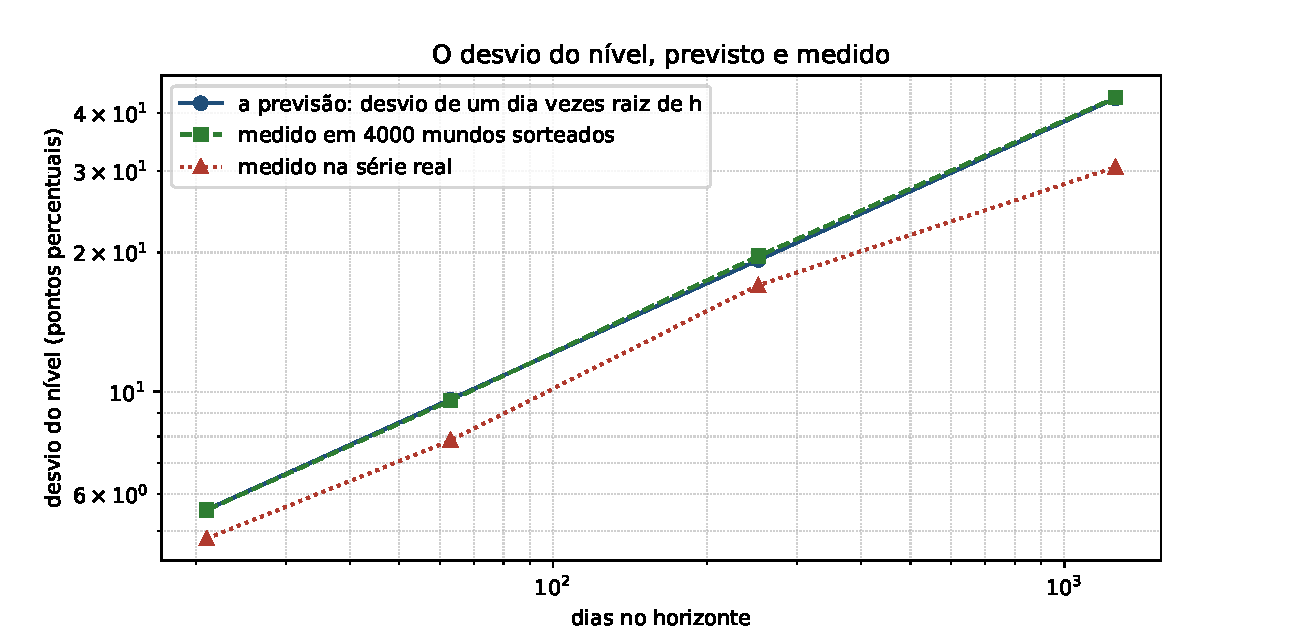
\includegraphics[width=\linewidth]{figuras/E22_soma_2.pdf}
  \caption{O desvio do nível contra o horizonte, nas três leituras. Os dois eixos estão em
    escala logarítmica, de modo que uma raiz aparece como reta de inclinação meio; a previsão e
    os mundos sorteados caem juntos, e a série real fica abaixo dos dois.}
  \label{fig:passo}
\end{figure}

A causa não está no tamanho dos dias: está na \textbf{ordem} deles. A autocorrelação de um dia nesta série vale
\numSomaRhoUm{} --- o dia de hoje tende a desfazer parte do que o de ontem andou ---, e a
previsão da raiz supõe justamente o contrário, dias independentes. Baralhando os retornos, de
modo que os mesmos dias enormes continuem todos lá e só a ordem morra, a razão no horizonte de um
mês vai a \numSomaBaralhadaRazaoVinteUm{} em \numSomaBaralhadaSorteios{} baralhamentos, contra
\numSomaRealVinteUmRazao{} do dado. Em cinco anos ela vai a
\numSomaBaralhadaRazaoMilDuzentosESessenta{}, e o que resta do buraco é do próprio estimador, que
mede janelas sobrepostas: a razão do horizonte longo é a de menor potência, e é a que menos
separa.

\begin{figure}[htbp]
  \centering
  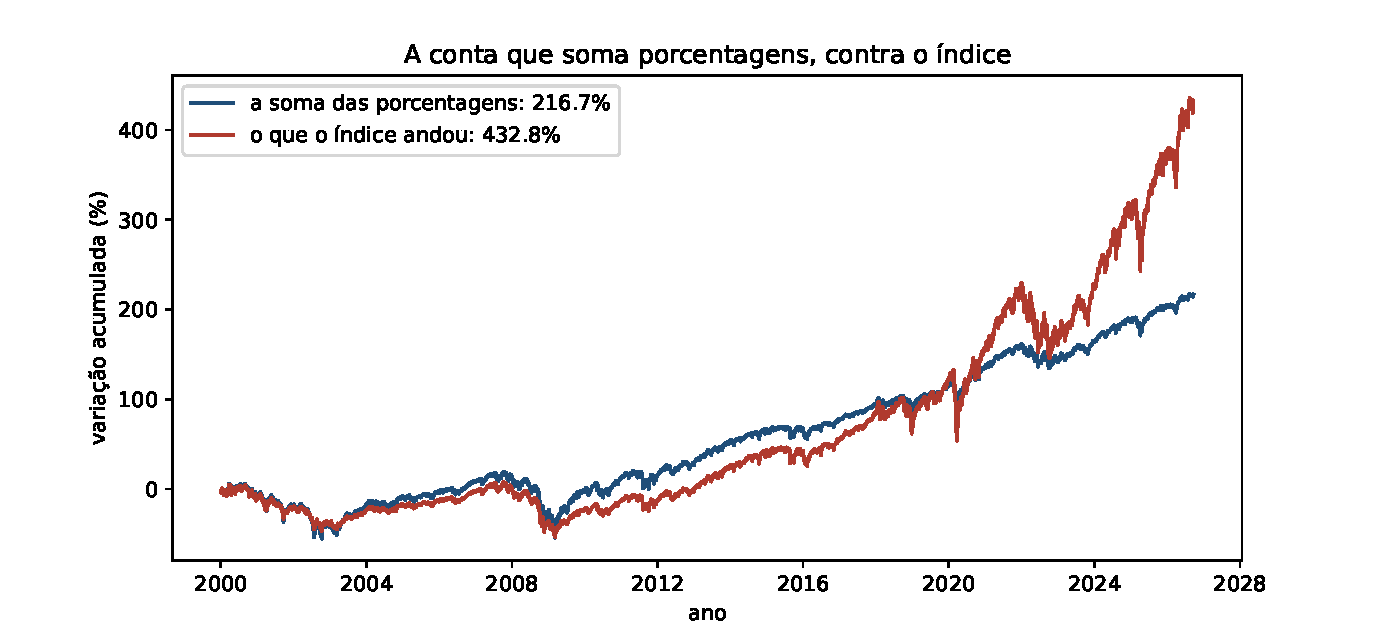
\includegraphics[width=\linewidth]{figuras/E22_soma_1.pdf}
  \caption{As duas somas, dia a dia, ao longo dos \numSomaSerieDias{} pregões. As curvas
    caminham juntas por anos, com a soma das porcentagens acima na maior parte do tempo, e se
    separam de vez no fim: o índice termina com mais que o dobro do que a soma entrega.}
  \label{fig:somas}
\end{figure}

O desenho mostra o mesmo que a conta: as duas curvas andam próximas por anos, e a distância
entre elas cresce com o tempo. Ela é pequena enquanto o nível anda pouco, e cresce com o
próprio nível --- que é o que uma multiplicação faz.

\section{A inclinação da banda em toda escala}

A seção anterior respondeu "quanto a banda da série fica abaixo da previsão" com um número
por horizonte --- e os quatro números dizem coisas diferentes, sem escada nenhuma entre eles.
Quem quer um número que valha para a série inteira tem a pergunta certa e o instrumento
errado: a razão num horizonte é uma leitura pontual, e a curva de \cref{fig:passo} tem
inclinação própria, esperando quem a meça.

% aterramento: atraso
% aterramento: passo-do-caminho
O instrumento mede o caminho em toda escala de uma vez. O \textbf{atraso} é o horizonte
entre os dois dias que entram na leitura: um dia, um mês de pregões, dois anos. O
\textbf{passo médio do caminho} é quanto o nível andou entre esses dois dias, em média ---
para cada atraso $h$, a média de $|\log p_{t+h} - \log p_t|$ sobre todas as janelas da
série, sobrepostas e sem dividir pelo atraso, o que é declaração: o que interessa é quanto o
passo cresce quando o atraso cresce. O exemplo mínimo cabe numa frase: no passeio puro,
quadruplicar o atraso dobra o passo médio.

A \cref{prop:passo} já contém essa frase. O passo típico de um passeio cresce com a raiz do
atraso, $\sigma\sqrt{h}$, de modo que contra o atraso em escala logarítmica o passo do
passeio é uma reta --- de inclinação um meio.

% aterramento: gama
A inclinação da reta é o objeto novo: o \textbf{expoente do caminho}, $\gamma$, um número
por série. E a leitura de Higuchi \cite{higuchi1988approach} é a de que essa inclinação é
um número repetível, que caracteriza a série que o produziu --- dita do outro lado, como
% aterramento: dimensao-do-caminho
dimensão: a \textbf{dimensão do caminho} é $2 - \gamma$. No sorteio puro a inclinação é meio
e a dimensão, três meios; caminhos mais lisos aproximam um, e caminhos que enchem a página
chegam a dois.

A medição corre nos três lugares de sempre: \numExpoenteMundos{} mundos do passeio puro, a
série, e os \numExpoenteSorteios{} baralhamentos da seção anterior --- o mesmo estimador,
os mesmos \numExpoenteAtrasos{} atrasos, de um dia a \numExpoenteAtrasoMaximo{} pregões, e
todo atraso com menos de \numExpoenteJanelasMinimas{} janelas de sobra fica de fora do
ajuste.

Nos mundos, a inclinação medida é \numExpoenteGammaPasseio{}, com dispersão
\numExpoenteGammaPasseioDispersao{} entre mundos --- meio, e a dimensão
\numExpoenteDimensaoPasseio{}, três meios. A régua da \cref{prop:passo}, agora como número
medido: \cref{fig:escala} mostra a régua caindo junto com o meio dos mundos.

Na série, o número é \numExpoenteGammaReal{} --- e a régua de ordem diz o que ele é. O
mesmo estimador nos baralhamentos dá \numExpoenteGammaBaralhadoMedia{}, com dispersão
\numExpoenteGammaBaralhadoDispersao{}: colado no da série, e as dimensões vêm coladas
junto, \numExpoenteDimensaoReal{} contra \numExpoenteDimensaoBaralhadoMedia{}. A inclinação global é carregada pelos tamanhos dos dias --- baralhar a ordem deixa o
número onde está. E a compressão que a
seção anterior mediu, a banda da série abaixo da prevista, mora na forma da curva, de um
jeito que o número global não vê --- a série nasce junto do baralhamento no atraso de um dia
(os mesmos dias), corre abaixo do meio dos mundos nos atrasos curtos e médios e a
alcança no maior deles; o baralhado, que também começa abaixo do meio dos mundos, o ultrapassa
na faixa curta. A \cref{fig:gamas} mostra o mesmo na contagem: as inclinações dos mundos se
acumulam no meio, as do baralhado um pouco à direita, e a linha da série cai dentro da
pilha do baralhado.

A forma aparece quando a inclinação é lida por faixa de atraso:

\begin{table}[htbp]
  \centering
  \small
  \resizebox{\linewidth}{!}{%
  \begin{tabular}{lrrr}
    \hline
    atrasos da faixa & a série & os mundos & o baralhado \\
    \hline
    um a oito dias & \numExpoenteGammaFaixaCurtaReal & \numExpoenteGammaFaixaCurtaPasseio & \numExpoenteGammaFaixaCurtaBaralhado \\
    dezesseis a sessenta e quatro & \numExpoenteGammaFaixaMediaReal & \numExpoenteGammaFaixaMediaPasseio & \numExpoenteGammaFaixaMediaBaralhado \\
    cento e vinte e oito a quinhentos e doze & \numExpoenteGammaFaixaLongaReal & \numExpoenteGammaFaixaLongaPasseio & \numExpoenteGammaFaixaLongaBaralhado \\
    \hline
  \end{tabular}}
  \caption{O expoente do caminho lido por faixa de atraso. Nos mundos, meio em toda faixa;
    na série, a inclinação anda com a escala; no baralhado, bem mais parada.}
  \label{tab:faixas}
\end{table}

Nos mundos a inclinação é meio em toda faixa --- a régua não depende da escala. Na série
ela anda: o dia que desfaz parte do dia anterior (\numSomaRhoUm{}) achata a faixa curta,
\numExpoenteGammaFaixaCurtaReal{} contra \numExpoenteGammaFaixaCurtaBaralhado{} do
baralhado --- a ordem, que o número global não via, aparece aqui ---, e na faixa longa a
série passa o próprio baralhado, \numExpoenteGammaFaixaLongaReal{} contra
\numExpoenteGammaFaixaLongaBaralhado. Entre os extremos, a inclinação sobe de
\numExpoenteGammaFaixaCurtaReal{} a \numExpoenteGammaFaixaLongaReal.

O que a inclinação entregou, e o que ela cobrou. Entregou: a régua de meio virou número
medido, a série ganhou o seu, e a régua de ordem disse do que o número é feito --- os
tamanhos dos dias. Cobrou: um número só descreve a série se a escala vier junto, e a ordem
dos dias, que decide a banda do mês, só aparece lendo faixa por faixa. O número que
caracteriza a série existe e é repetível; descrever a série com ele é outra história.

\begin{figure}[htbp]
  \centering
  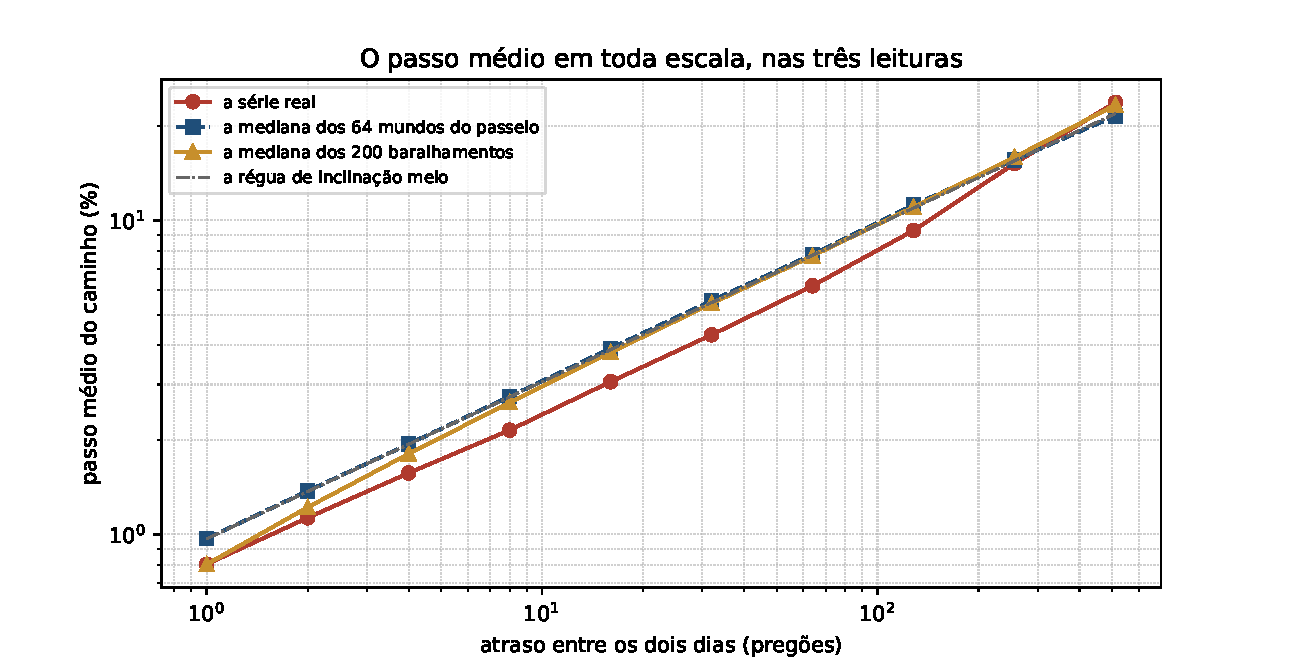
\includegraphics[width=\textwidth]{figuras/E44_expoente_1.pdf}
  \caption{O passo médio do caminho contra o atraso, nos dois eixos em escala logarítmica.
    A série nasce junto do baralhamento no atraso de um dia --- os mesmos dias ---, corre
    abaixo do meio dos mundos nos atrasos curtos e médios e a alcança no maior deles; o
    baralhado começa abaixo do meio dos mundos e o ultrapassa dentro da faixa curta; a régua de
    meio cai junto com o meio dos mundos.}
  \label{fig:escala}
\end{figure}

\begin{figure}[htbp]
  \centering
  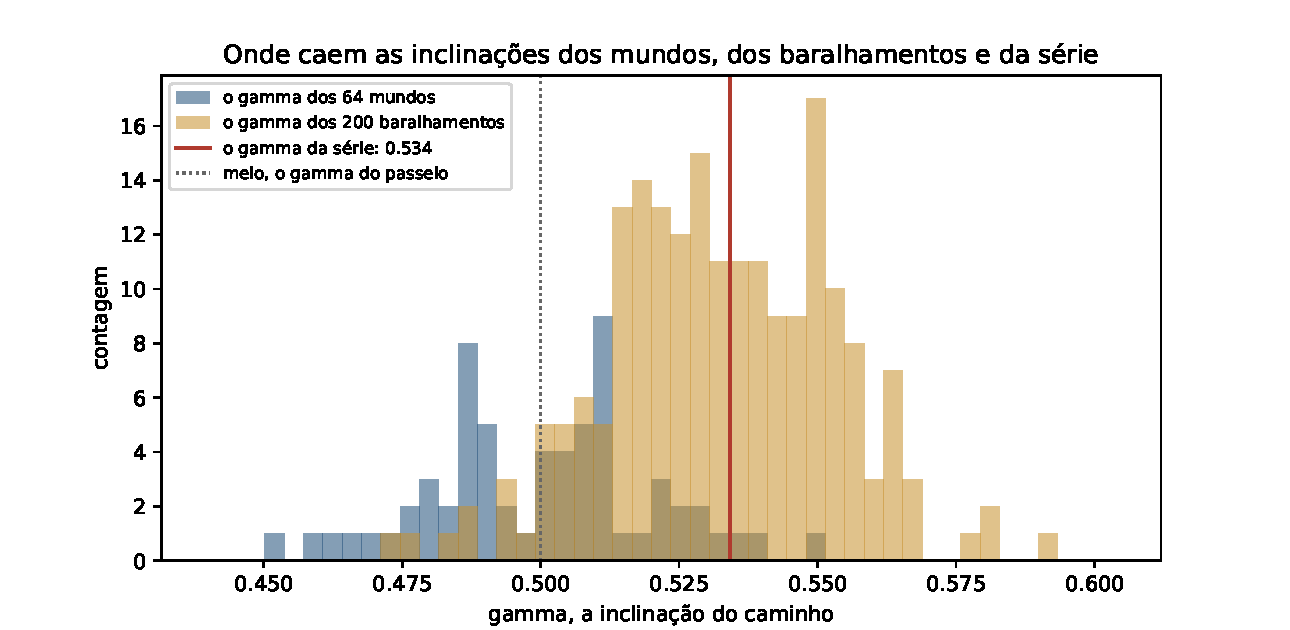
\includegraphics[width=\textwidth]{figuras/E44_expoente_2.pdf}
  \caption{A inclinação de cada mundo e de cada baralhamento, com a da série marcada. As
    pilhas se acumulam perto de meio --- a dos mundos em cima dele, a do baralhado um pouco
    à direita --- e a linha da série cai dentro da pilha do baralhamento: o expoente global
    é um número dos tamanhos dos dias.}
  \label{fig:gamas}
\end{figure}

\section{O que fica}

Ficam os dois objetos que o resto do livro usa sem dizer: o \textbf{nível}, que é o preço, e o
\textbf{incremento}, que é o que o dia acrescentou. Fica a ponte entre eles, e ela é o
logaritmo: somar retornos é o mesmo que olhar a razão entre dois preços, exatamente. E fica a
banda do nível, que cresce com a raiz do horizonte --- medida em \numSomaMundos{} mundos, e
posta contra o dado real, onde ela exagera porque o dia de hoje desfaz parte do que o de
ontem andou.

A pergunta da noite continua de pé, e agora se vê o tamanho dela. A banda do nível se alarga
com o horizonte, e o que se quer saber é quanto se pode perder amanhã: uma resposta que não
pode ser uma linha fixa, porque a linha não se alarga. Medir o dia ruim exige erguer uma linha
sobre os piores dias do passado e olhar o que ficou abaixo dela --- e é essa linha que o
capítulo seguinte constrói.

% =============================================================================
% CAPÍTULO 3 — a raiz (AGENTS.md §6): a medida, o corte e o preço de fixar.
%
% O fracasso que o abre, com número na mão: a linha erguida no décimo terceiro pior
% dia dos últimos 252 pregões entrega 5,135% contra os 5% anunciados — parece
% cumprida —, mas o pior bloco de 60 dias tem 20 violações onde a promessa admitia
% 3, e nenhum dos 200 mundos que nunca mudam passou de 13.
%
% Medição: lab/experimentos/E01_promessa.ipynb. Figuras: figuras/E01_promessa_*.
% =============================================================================

\chapter{A medida, o corte e o preço}
\label{cap:medida}

\section{Quanto eu posso perder amanhã}

O mercado fecha, e a pergunta volta quase toda noite com as mesmas palavras: quanto eu posso
perder amanhã? Quem carrega dinheiro aplicado não pergunta por gosto de adivinhar, porque a
resposta decide se a posição cabe no bolso de quem a carrega; e a posição que não cabe acaba
desmontada, muitas vezes antes de o mercado explicar o que estava acontecendo.

Responder exige duas decisões, e as duas são sobre o passado. A primeira é quantos dias olhar
para trás. A segunda é onde pôr a linha dentro desses dias, que podem ser o pior de todos, o
segundo pior, o décimo terceiro. Escrita por inteiro, a regra soa assim: \emph{o corte de hoje
é o décimo terceiro pior dia dos últimos \numCorteJanela{} pregões}. Ela também traz o que
pretende valer: \emph{não passo daqui, dezenove dias em vinte}, que é o mesmo que prometer
\numPromessaPct\% de violação.

Vale fixar quatro palavras, porque nenhuma delas muda de sentido daqui em diante: a
\textbf{janela} é o pedaço do passado que a regra olha; o \textbf{corte} é onde a linha é posta
dentro da janela; a \textbf{promessa} é a taxa de violação que se anuncia; e a \textbf{entrega}
é a taxa que de fato acontece.

A linha posta no quantil dos piores dias sustenta a medida de risco mais usada em finanças,
discutida e corrigida há décadas \cite{oconnell2026extreme}.
% aterramento: quantil
O quantil de uma fração declarada é o valor que deixa essa fração dos dias abaixo dele, e é ele
que o corte usa aqui. Com cem dias e a fração de um quinto, o quantil é o vigésimo pior dia:
vinte dos cem ficam abaixo dele. O que se pergunta vem antes disso, e é bem menor: a entrega tem
alguma coisa a ver com a promessa?

\section{O dado e a regra}

O dado é o retorno de um dia para o outro, que o capítulo anterior escreveu como o logaritmo
da razão entre dois preços:

\[
  r_{t+1} = \log \frac{p_{t+1}}{p_t}.
\]

O retorno é o incremento e o preço é o nível: empilhar dias é somar retornos, e é isso que
permite acompanhar o dia a dia sem perder o fio da conta.

A série é o índice S\&P 500, % numeros-ok: nome próprio, não medição
com \numSerieDias{} pregões, de \numSerieInicio{} a \numSerieFim. Ela vem do arquivo do
projeto anterior, e o empréstimo fica declarado: o dado atravessa, e todo número tirado dele é
medido de novo aqui.

Sobre essa série a regra toma duas decisões, e só duas. A \textbf{janela}: os
\numCorteJanela{} pregões anteriores a hoje. O \textbf{corte}: o décimo terceiro pior deles.
O corte de cada dia é erguido com os dias que já passaram e com nenhum outro, de modo que a
linha que aparece no gráfico estava lá antes de o dia acontecer. Um corte que espiasse o
futuro acertaria sempre, e por isso não valeria nada.

\section{A conta que o corte faz sozinho}

Nos \numEntregaDias{} dias em que havia janela suficiente, a linha foi rompida
\numEntregaViolacoes{} vezes. Isso dá \numEntregaTaxaPct\% de entrega, contra os
\numPromessaPct\% anunciados, uma diferença de pouco mais de um décimo de ponto percentual, pequena o
bastante para deixar a impressão de que a regra funcionou.

A impressão engana, e o motivo é aritmético. Quem decidiu o número foi o gesto de erguer a
linha dentro da janela, e não o que o mercado fez depois.

% aterramento: k
% aterramento: n
Vale dar nome às duas peças da decisão, porque a conta inteira se escreve com elas: $n$ é o
número de dias da janela, e $k$ é o posto do corte dentro dela --- o lugar que a linha ocupa na
fila dos piores dias. O corte é o décimo terceiro pior, de modo que aqui $k$ é treze e $n$ é
\numCorteJanela.

\begin{proposicao}[a conta do corte]
\label{prop:conta}
Suponha que os $n$ dias da janela e o dia seguinte sejam $n+1$ valores de uma mesma lei
contínua, em qualquer ordem igualmente provável. Se o corte é o $k$-ésimo menor dos $n$
dias da janela, então a probabilidade de o dia seguinte ficar abaixo do corte é
$\dfrac{k}{n+1}$.
\end{proposicao}

\begin{proof}
Junte os $n+1$ valores e ponha-os em ordem crescente. Todas as ordens são igualmente
prováveis, então a posição do dia seguinte nessa fila é uniforme entre as $n+1$ posições. O
dia seguinte fica abaixo do corte exatamente quando ocupa uma das $k$ primeiras posições da
fila dos $n+1$ valores. Logo a probabilidade é $k/(n+1)$.
\end{proof}

A lei ser contínua serve para que dias empatados tenham probabilidade zero; e a hipótese de
que todas as ordens são igualmente prováveis é a hipótese de que os dias não têm nada a dizer
uns sobre os outros, que é justamente o que um mundo que muda viola\cite{vovk2022algorithmic}. A proposição não prevê o
que vai acontecer. Ela é o contraste contra o qual o que aconteceu se lê.

Ela também é um caso pequeno e exato de um viés conhecido. Uma \textbf{amostra} é o pedaço
finito de dias de que se dispõe --- aqui, a janela ---, e um \textbf{viés} é o erro que a própria
regra assina antes de o dado chegar, e que por isso não vem do mundo.
% aterramento: amostra
% aterramento: vies
O quantil estimado de uma amostra não entrega a probabilidade que se anuncia, e o tamanho do
erro depende do tamanho da amostra \cite{taleb2020super}.

Com $n = \numCorteJanela$ e $k = \numCortePosto$, a conta dá
$\numCortePosto/(\numCorteJanela+1)$, que é \numCorteContaPct\%. Esse número não veio do
mercado, e sim da decisão de olhar \numCorteJanela{} dias e cortar no décimo terceiro. Se o
posto fosse o décimo segundo, a conta daria \numCorteAlternativoPct\%; e a promessa anunciada
não está em nenhum dos dois, porque o posto teria de cair entre o décimo segundo e o décimo
terceiro, e posto fracionário não existe.

O mercado entregou \numEntregaTaxaPct\%: \numEntregaViolacoes{} rompimentos em
\numEntregaDias{} dias, com poucos milésimos de diferença da conta do corte. Para saber se
essa diferença diz alguma coisa, falta o contraste que responde, e ele pede um mundo em que
nada muda submetido à mesma rotina.
% aterramento: mundo-parado
A esse contraste dou um nome, porque ele volta quase toda vez daqui em diante: o \textbf{mundo
que nunca muda}.

Sorteamos \numNuncaMudaMundos{} séries do tamanho da nossa, com retornos independentes e
sempre a mesma lei, e aplicamos a cada uma a mesma regra. A entrega média desses mundos foi
\numNuncaMudaTaxaPct\%, contra os \numCorteContaPct\% da conta; o mundo real entregou
\numEntregaTaxaPct\%. Os três números estão no mesmo lugar.

A média de violações é uma propriedade do corte, e não do mundo. O corte assinou o número
antes de qualquer dado chegar, e quem lê só a média lê a própria escolha acreditando estar
lendo o mercado.

\section{Os blocos têm data}

A diferença entre os mundos aparece na \emph{forma} com que as violações chegam: espalhadas
pelo calendário, ou concentradas em pedaços. Para medir a forma, contamos quantas violações
caem em cada janela móvel de \numBlocoDias{} dias --- a isso chamamos um \textbf{bloco} ---
e olhamos o bloco mais cheio. A promessa de \numPromessaPct\% admite \numBlocoPrometido{}
violações em \numBlocoDias{} dias.

% aterramento: mediana
A mediana dos blocos é \numBlocoMediana. A mediana é o quantil de metade: metade dos blocos tem
menos violações que ela, e a outra metade tem mais. Na maior parte do tempo a linha aguenta mais
do que prometeu. O pior bloco tem \numBlocoPior{} violações, e termina em \numBlocoPiorData. Onde a
promessa admitia \numBlocoPrometido{}, aconteceram \numBlocoPior.

Nos \numNuncaMudaMundos{} mundos que nunca mudam, o pior bloco de cada um teve, em média,
\numNuncaMudaPiorMedio{} violações, e o pior bloco de todos eles chegou a
\numNuncaMudaPiorBloco. Nenhum passou disso. A série real, com o mesmo tamanho e a mesma
rotina, chegou a \numBlocoPior.

\begin{figure}[htbp]
  \centering
  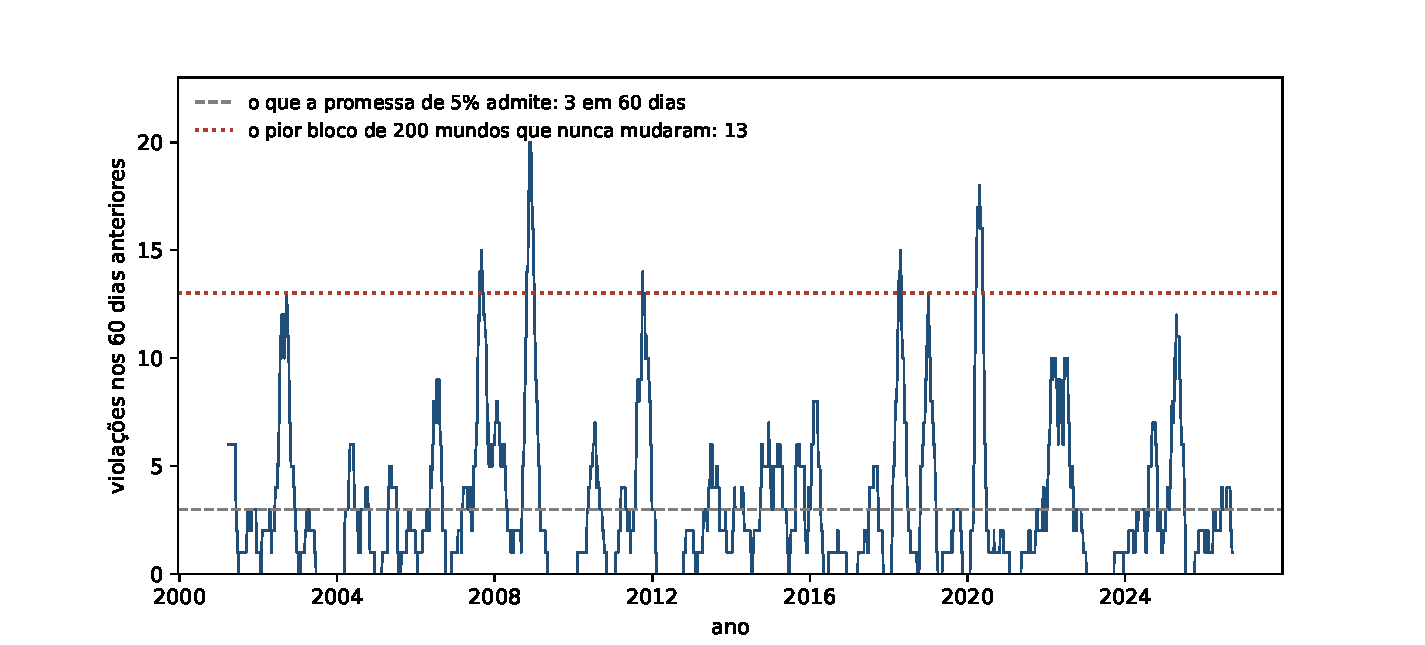
\includegraphics[width=\linewidth]{figuras/E01_promessa_1.pdf}
  \caption{Violações nos \numBlocoDias{} dias anteriores, dia a dia. A linha tracejada marca o
    que a promessa de \numPromessaPct\% admite; a pontilhada marca o pior bloco que apareceu
    em \numNuncaMudaMundos{} mundos que nunca mudam.}
  \label{fig:blocos}
\end{figure}

A escala do desenho trabalha contra a leitura. A linha da promessa fica rente ao chão do quadro, e é
ali que a série passa a maior parte do tempo; um eixo cortado perto dela devolveria um desenho de
promessa cumprida, e os surtos que cruzam o teto desapareceriam por recorte.

A figura mostra o que a média esconde. A série passa trechos longos colada na linha da
promessa e sobe, em surtos curtos, até cruzar a linha pontilhada. E os blocos têm data: o teto
dos mundos que nunca mudam é cruzado em \numEpisodiosAcimaDoTeto{} episódios distintos, dois deles em dois mil e
sete, que ocupam \numBlocosAcimaDoTetoPct\% dos blocos medidos, em \numEpisodiosAnos. Nem todos esses
anos têm nome de crise, e todos aconteceram neste mercado.

A leitura do bloco corrige ainda a primeira impressão: \numBlocoAcimaDoDobroPct\% dos blocos
passam do dobro da promessa. O que se promete fica longe do que se entrega, tanto na maior
parte do tempo quanto nos piores pedaços, e a entrega acaba sendo uma média entre os dois.

\section{O preço muda de lugar}

Se o corte assina a média, uma saída parece evidente: escolher outra janela. Vale a pena
tentar, e a tentativa é barata, porque é a mesma regra com outro número. Varremos a janela de
um mês a cinco anos, mantendo a promessa anunciada de \numPromessaPct\% e o bloco de
\numBlocoDias{} dias.

\begin{table}[htbp]
  \centering
  \begin{tabular}{rrrr}
    \hline
    janela & a conta do corte & a entrega & o pior bloco \\
    (pregões) & (\%) & (\%) & (violações) \\
    \hline
    \numCorteCurtoJanela & \numCorteCurtoContaPct & \numCorteCurtoTaxaPct & \numCorteCurtoPiorBloco \\
    \numCorteMedioJanela & \numCorteMedioContaPct & \numCorteMedioTaxaPct & \numCorteMedioPiorBloco \\
    \numCorteJanela & \numCorteContaPct & \numEntregaTaxaPct & \numBlocoPior \\
    \numCorteLongoJanela & \numCorteLongoContaPct & \numCorteLongoTaxaPct & \numCorteLongoPiorBloco \\
    \hline
  \end{tabular}
  \caption{A mesma regra com quatro janelas, a mesma promessa anunciada de
    \numPromessaPct\% e o mesmo bloco de \numBlocoDias{} dias. A coluna do meio segue a
    \cref{prop:conta}; a última traz o pior bloco medido.}
  \label{tab:varredura}
\end{table}

As três colunas respondem à pergunta do começo.

A \textbf{conta do corte} obedece à promessa anunciada apenas na janela longa. Na janela de um
mês, o corte assina \numCorteCurtoContaPct\%, quase o dobro dos \numPromessaPct\% anunciados,
e a razão disso é aritmética pura, porque com poucos dias não existe posto que produza
\numPromessaPct\%.

A \textbf{entrega} acompanha a conta do corte nas quatro janelas, e fica acima dela em três; na janela de
\numCorteJanela{} as duas praticamente coincidem. Esse resto é a contribuição do mundo, e é pequeno. Encurtar a janela entrega uma medida
mais grosseira e uma promessa mais cara.

O \textbf{pior bloco} caminha no sentido oposto: \numCorteCurtoPiorBloco,
\numCorteMedioPiorBloco, \numBlocoPior, \numCorteLongoPiorBloco. Quanto mais longo o passado
que a linha olha, mais tempo ela leva para acompanhar o que mudou, e mais violações cabem no
pedaço ruim. Na janela de cinco anos o pior bloco chega a \numCorteLongoPiorBloco. No extremo
oposto, uma janela curta não compra bloco nenhum, e o pior bloco do mundo real,
\numCorteCurtoPiorBloco, fica \emph{abaixo} do pior bloco de um mundo que nunca muda, porque
uma janela curta se move junto com o mercado --- e cobra o preço na média.

\begin{figure}[htbp]
  \centering
  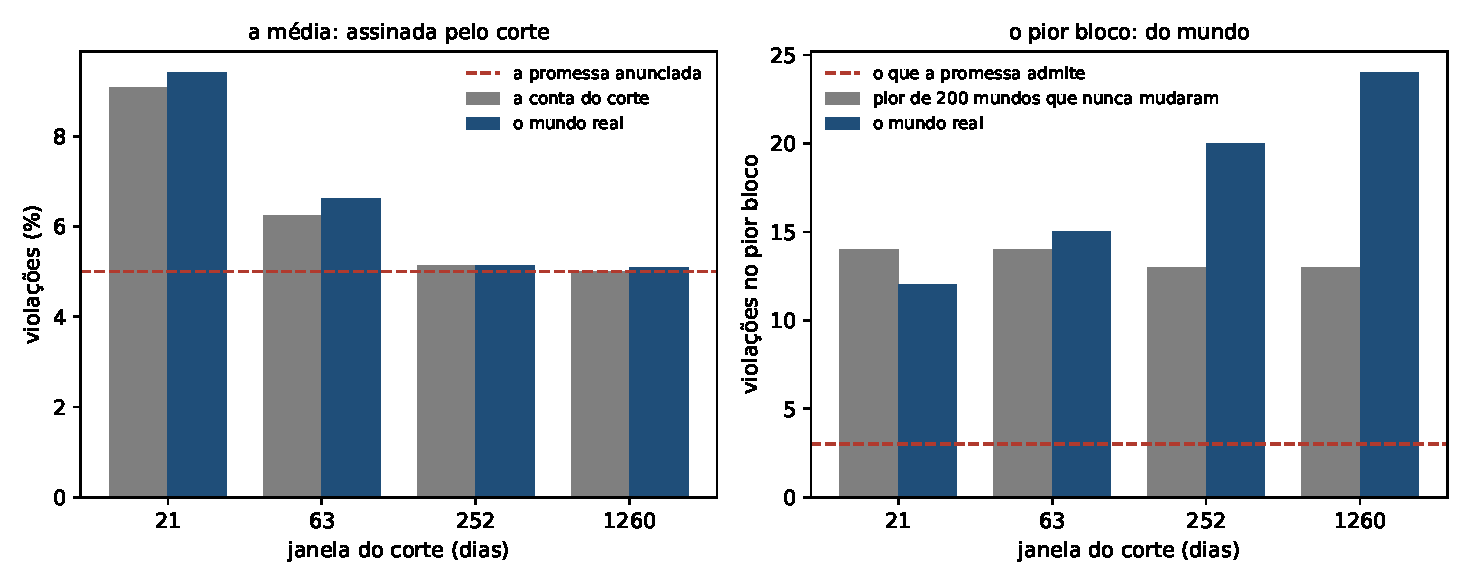
\includegraphics[width=\linewidth]{figuras/E01_promessa_2.pdf}
  \caption{As duas leituras, nas quatro janelas. À esquerda, a média: a conta do corte e o
    mundo real andam juntos. À direita, o pior bloco: o mundo real contra o pior dos
    \numNuncaMudaMundos{} mundos que nunca mudam.}
  \label{fig:duas}
\end{figure}

Encurtar o corte cobra na média; alongá-lo cobra no bloco. Não há janela em que a linha
entregue o que a promessa anunciou, e a razão disso está na \cref{prop:conta}, que não deixa o
mundo entrar na conta.

\section{Uma linha erguida no passado}

Um corte fixo supõe que o pedaço de passado que ele olha se parece com o pedaço que vem. A
série deixa de se parecer consigo mesma: passa meses colada na linha e depois rompe a linha
\numBlocoPior{} vezes em \numBlocoDias{} dias, com o pior bloco terminando em
\numBlocoPiorData.

Quando isso acontece, a linha erra por muito. Ela foi erguida com os dias de antes, e são
justamente esses dias que deixaram de valer. A \cref{tab:varredura} já mostrava o mesmo por
outro caminho, porque quanto mais longo o passado que a linha olha, mais tempo ela leva para
acompanhar o que mudou, e mais violações cabem no pedaço ruim.

Se os blocos têm data, alguma coisa no mundo se move, e a média olha para outro lugar. Resta
medir essa mudança, e os capítulos seguintes fazem isso.

\section{O que fica}

Fica o instrumento, e ele é uma linha: o $k$-ésimo pior dos últimos $n$ dias, que assina a taxa
$k/(n+1)$ antes de qualquer dado chegar. Fica também o primeiro preço medido do livro: o corte
entrega \numCorteContaPct\% onde a promessa era de \numPromessaPct\%, e essa média não distingue
o mercado de um mundo que nunca muda.

O que distingue os dois é a forma com que as violações chegam. Nos mundos que nunca mudam o pior
bloco de \numBlocoDias{} dias parou em \numNuncaMudaPiorBloco; aqui ele chegou a \numBlocoPior, em
\numBlocoPiorData.

E fica a pergunta que abre todo o resto: um corte fixo vale enquanto o passado se parecer com o que
vem, e este capítulo mostrou que ele não se parece. Medir essa mudança, e o que se pode fazer com
um alarme que chega depois dela, é o que vem.

\part{As voltas}

Com o corte na mão, o instrumento ganha orçamento e o mundo ganha formas. A mesma linha é
vigiada com um alarme declarado, e a mudança chega de maneiras diferentes: a cauda que se abre
de uma vez, a rampa que se aproxima devagar, a média que se desloca, o relógio da semana e a
outra perna do par. Cada forma cobra do mesmo silêncio um preço diferente.

% =============================================================================
% CAPÍTULO 4 — volta 1 (AGENTS.md §6): o orçamento do alarme.
%
% O fracasso que o abre, com número na mão: o vigia do capítulo 3, ligado no limiar que o
% mundo parado não ultrapassa, soa uma vez a cada 3632 anos de mundo parado e avisa do
% tombo de 2020 com 86% do prejuízo já pago. A troca entre silêncio e antecedência é a
% curva da fig:troca; o atraso tem piso provado (prop:piso); o orçamento se compra com
% memória (1/(n+1)) — e a forma da mudança, que decide o preço desse silêncio, é o capítulo
% seguinte.
%
% Medição: lab/experimentos/E02_orcamento.ipynb. Figuras: figuras/E02_orcamento_1 e _2.
% =============================================================================

\chapter{O orçamento do alarme}
\label{cap:orcamento}

\section{O vigia}

O capítulo anterior deixou um instrumento e um incômodo. O instrumento conta quantas vezes o
preço rompeu a linha dentro de uma janela móvel de \numVigiaBloco{} dias. O incômodo é que os
blocos têm data: a contagem sobe nos mesmos anos, e sobe sempre no mesmo lugar da série.

A tentação, agora, é pequena e razoável. Se o bloco sabe \emph{quando} o mundo aperta, basta
ligar nele um alarme: soa quando a contagem passa de um limiar. E o limiar já vem escolhido
por medição, não por gosto, porque no capítulo anterior o pior bloco de duzentos mundos que
nunca mudam chegou a \numNuncaMudaPiorBloco{} violações. Um número que o mundo parado não
ultrapassa é um candidato honesto a linha de alarme --- e \numVigiaMundosQueSoamPct\% dos mundos
parados o alcançam, um em cada duzentos.

Fica então o vigia mais simples que dá para escrever: \emph{soa quando as violações dos
últimos \numVigiaBloco{} dias chegam a \numVigiaLimiar}.

Duas perguntas decidem se isso vale alguma coisa, e o capítulo é sobre elas: com que
frequência ele soa quando nada muda, e quanto tempo ele leva quando algo muda de verdade. As
duas precisam de resposta junta, porque cada uma é paga com a outra \cite{wald1945sequential}.

\section{Quanto ele soa quando nada muda}

% aterramento: falso-alarme
A primeira pergunta não se responde no mercado, porque no mercado não se sabe quais alarmes
eram falsos. Sabe-se que houve alarme, e só. O alarme que soa num mundo que não mudou tem nome
--- é o \textbf{falso alarme} ---, e a frequência com que ele soa é o orçamento do vigia.
Responde-se em mundos em que nada muda:
\numVigiaMundos{} séries do tamanho da nossa, com retornos independentes e sempre a mesma
lei, submetidas ao mesmo corte, aos mesmos blocos e ao mesmo limiar.

No limiar \numVigiaLimiar{}, essas mil séries produziram \numVigiaDiasParadoPorMundo{} dia de
alarme por mundo --- quase nada ---, e \numVigiaMundosQueSoamPct\% dos mundos soaram pelo
menos uma vez ao longo de vinte e cinco anos. Dito em tempo: o vigia soa sozinho uma vez a
cada \numVigiaAnosParadoPorAlarme{} anos.

Um número desses pede desconfiança, e a desconfiança aqui é aritmética. Ele se apoia em
\numVigiaParadoAlarmes{} alarmes espalhados por \numVigiaMundos{} mundos; contar evento raro
é impreciso, e o erro relativo dessa contagem é de \numVigiaParadoErroPct\%. O que a medição
entrega é a ordem de grandeza --- milhares de anos ---, e não o número exato.

Há um jeito de conferir esse orçamento sem sortear nada, e ele cabe numa proposição, porque a
conta é uma união de acontecimentos.

% aterramento: prob
% aterramento: A
% aterramento: binomial
% aterramento: B
% aterramento: L
Escrevo $\Prob(A)$ para a probabilidade do acontecimento $A$. Falta nomear as peças do bloco:
ele tem $B$ dias, cada um com a probabilidade $p$ de violar o corte, e o alvo é $L$ violações.
A contagem dentro de um bloco de $B$ dias independentes é a soma de $B$ indicadores --- o mesmo indicador
do dia que a barra da média usou ---, de modo que a chance de ela alcançar $L$ é a cauda dessa soma, que se escreve
$\Prob\big(\text{Bin}(B, p) \geq L\big)$ e se lê assim: a probabilidade de a contagem de
$B$ sorteios independentes, cada um com probabilidade $p$, chegar a $L$.

\begin{proposicao}[o teto independente]
\label{prop:teto}
Se os dias fossem independentes, com probabilidade $p$ de violar o corte em cada dia, então a
probabilidade de algum bloco de $B$ dias atingir $L$ violações não passaria de
$n \cdot \Prob\big(\text{Bin}(B, p) \geq L\big)$, onde $n$ é o número de blocos.
\end{proposicao}

\begin{proof}
O acontecimento \emph{algum bloco atinge o limiar} é a união, sobre os $n$ blocos, dos
acontecimentos \emph{este bloco atinge o limiar}. A probabilidade de uma união nunca excede a
soma das probabilidades dos seus termos, e sob independência a probabilidade de um bloco
atingir $L$ violações é a cauda da binomial.
\end{proof}

Com os números do vigia o teto dá \numVigiaTetoIndependentePct\%, e o mundo parado
mediu \numVigiaMundosQueSoamPct\%. O teto está acima do medido, como tinha de estar, e está
acima por quase uma dezena de vezes: é um limite provado e frouxo, e vale pelo que prova.

Ele também tem prazo de validade, e o prazo aparece na própria conta. Para limiares baixos a
soma das parcelas ultrapassa cem por cento, e um teto que passa de cem por cento não é teto de
nada.

\section{Quanto ele demora quando algo muda}

O orçamento sozinho não decide nada. A pergunta que decide é a outra: quando o mundo muda, o
vigia avisa a tempo de quê?

Na série inteira, e no mesmo limiar, ele soou \numVigiaAlarmesReais{} vezes em vinte e cinco
anos, uma a cada \numVigiaAnosReaisPorAlarme{} anos. No mundo parado o mesmo vigia soa uma vez
a cada \numVigiaAnosParadoPorAlarme{} anos, ou \numVigiaRazaoRealContraParado{} vezes mais
raro. Quem soa uma vez a cada três anos e meio num mundo que muda está respondendo ao mundo, e
não ao próprio ajuste.

Para medir a que ele responde, cada alarme é comparado com o topo anterior e o fundo seguinte
--- o preço mais alto antes do tombo e o mais baixo depois ---, e a conta que interessa é
quanto do prejuízo total já tinha acontecido no dia do aviso.

Nos dois tombos maiores do período, o resultado é este.

\begin{table}[htbp]
  \centering
  \begin{tabular}{lrrr}
    \hline
    & atraso desde o topo & prejuízo já pago \\
    \hline
    alarme de \numVigiaTomboAntigoData & \numVigiaTomboAntigoAtrasoDias{} dias & \numVigiaTomboAntigoPagoPct\% \\
    alarme de \numVigiaTomboRecenteData & \numVigiaTomboRecenteAtrasoDias{} dias & \numVigiaTomboRecentePagoPct\% \\
    \hline
  \end{tabular}
  \caption{Os dois piores tombos do período, com o dia do alarme e a fração do prejuízo total
    que já tinha acontecido quando ele soou. No tombo mais recente, o alarme veio com
    \numVigiaTomboRecenteQuedaPct\% de queda já realizada, de um total de
    \numVigiaTomboRecenteTotalPct\%.}
  \label{tab:atraso}
\end{table}

A mediana dos \numVigiaAlarmesReais{} alarmes é de \numVigiaPagoMedianoPct\% de prejuízo já
pago. Num deles o alarme soou no fundo exato, com \numVigiaPagoPiorPct\% do tombo consumido:
o vigia avisou no dia em que a queda acabou.

Vale dizer do modo mais direto possível. O vigia acerta: os alarmes dele são reais, e o mundo
parado quase nunca o faz soar. O que ele não faz é chegar antes.

\section{A troca}

Se o vigia é tardio, a saída parece óbvia: baixar o limiar. Baixar o limiar antecipa o alarme
e cobra por isso, e o que vale medir é quanto, porque o preço tem forma.

Para cada limiar medimos as duas coisas de uma vez: a frequência com que ele soa em mundo
parado, e quanto do prejuízo já estava pago quando ele soou no tombo recente.

\begin{table}[htbp]
  \centering
  \begin{tabular}{rrr}
    \hline
    limiar & um alarme falso a cada & prejuízo já pago no tombo recente \\
    (violações) & (anos de mundo parado) & (\%) \\
    \hline
    \numTrocaOitoLimiar & \numTrocaOitoAnos & \numTrocaOitoPagoPct \\
    \numTrocaNoveLimiar & \numTrocaNoveAnos & \numTrocaNovePagoPct \\
    \numTrocaDezLimiar & \numTrocaDezAnos & \numTrocaDezPagoPct \\
    \numTrocaOnzeLimiar & \numTrocaOnzeAnos & \numTrocaOnzePagoPct \\
    \numTrocaDozeLimiar & \numTrocaDozeAnos & \numTrocaDozePagoPct \\
    \numVigiaLimiar & \numTrocaTrezeAnos & \numTrocaTrezePagoPct \\
    \hline
  \end{tabular}
  \caption{A troca, medida. Baixar o limiar antecipa o alarme e multiplica o falso alarme; a
    taxa de câmbio não é constante, e piora à direita da tabela.}
  \label{tab:troca}
\end{table}

A tabela diz três coisas.

\textbf{A troca existe, e o primeiro passo é barato.} Baixar o limiar de \numVigiaLimiar{}
para \numTrocaOitoLimiar{} derruba o prejuízo já pago de \numTrocaTrezePagoPct\% para
\numTrocaOitoPagoPct\%: o vigia passa a avisar antes de o tombo se completar.

\textbf{O preço desse passo é brutal.} O mesmo movimento leva o falso alarme de um a cada
\numTrocaTrezeAnos{} anos de mundo parado para um a cada \numTrocaOitoAnos{} anos. O vigia que
quase nunca se enganava passa a soar a cada poucos anos sem que nada tenha mudado.

\textbf{E a taxa de câmbio piora na outra ponta.} Do limiar \numTrocaDezLimiar{} para o
\numTrocaDozeLimiar, o falso alarme fica quase vinte vezes mais raro e o prejuízo já pago sobe
de \numTrocaDezPagoPct\% para \numTrocaDozePagoPct\%: trinta pontos de prejuízo comprados com
silêncio. E há dois limiares vizinhos entregando quase a mesma coisa --- o \numTrocaDozeLimiar{} e o
\numVigiaLimiar, com \numTrocaDozePagoPct\% contra \numTrocaTrezePagoPct\%.

\begin{figure}[htbp]
  \centering
  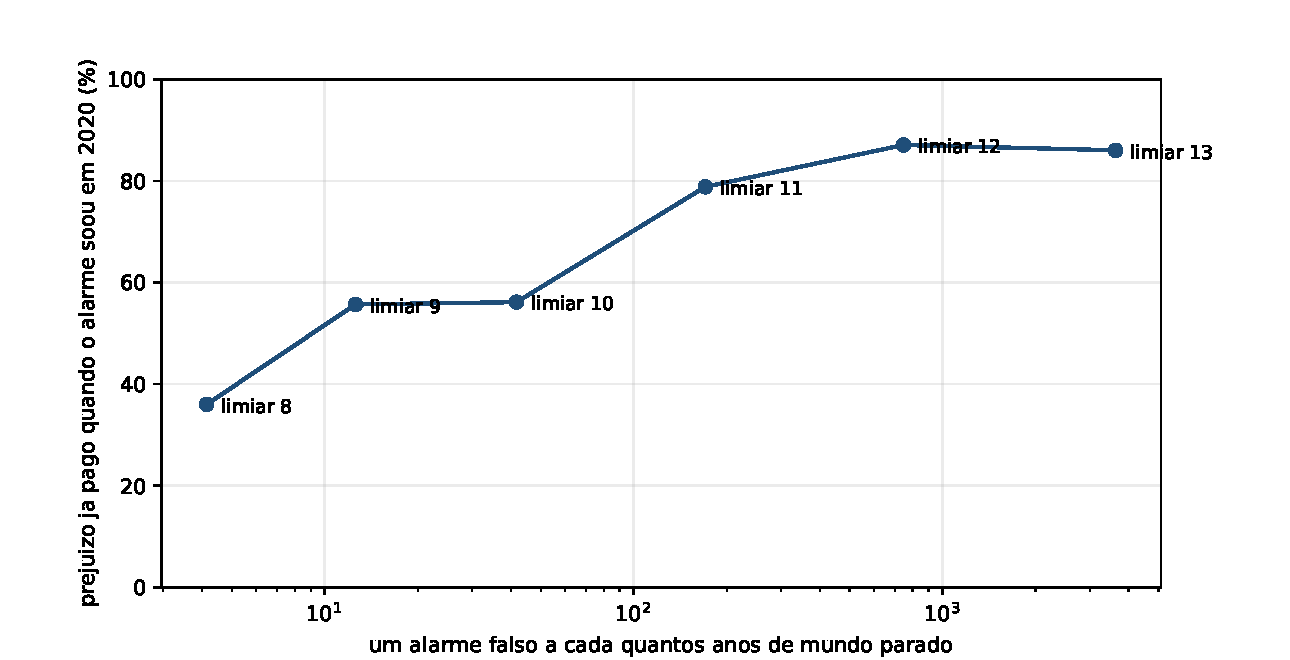
\includegraphics[width=\linewidth]{figuras/E02_orcamento_1.pdf}
  \caption{A troca em forma de curva: o eixo horizontal é a raridade do falso alarme, em
    escala logarítmica, e o vertical é o prejuízo já pago no tombo recente. A curva sobe
    depressa na esquerda e achata na direita.}
  \label{fig:troca}
\end{figure}

Não existe limiar que seja ao mesmo tempo raro e rápido. O vigia é o par --- frequência em
mundo parado e atraso em mundo que muda ---, e escolher um limiar é escolher um ponto dessa
curva, com o preço da esquerda pago em falso alarme e o da direita pago em atraso.

\section{O piso}

Antes de concluir que o vigia está mal calibrado, vale olhar o chão em que ele está, porque o
atraso dele tem piso, e o piso é aritmético.

\begin{proposicao}[o piso do atraso]
\label{prop:piso}
Um alarme que exige $L$ violações dentro da janela móvel não pode soar antes de $L-1$ pregões
depois de a mudança começar, se antes dela o corte não era violado.
\end{proposicao}

\begin{proof}
Para que a contagem chegue a $L$, são necessários ao menos $L$ dias com violação dentro da
janela. Cada dia com violação consome um pregão, e nenhum deles pode ser anterior ao começo da
mudança --- que é um dia mudado, e já pode violar. Contando o dia da mudança como zero, o alarme
não pode soar antes de $L-1$ pregões.
\end{proof}

Com $L = \numVigiaLimiar$, o piso é de \numVigiaPisoPregoes{} pregões. O alarme de
\numVigiaTomboRecenteData{} soou \numVigiaTomboRecenteAtrasoDias{} dias corridos depois do
topo: o vigia não estava gastando tempo à toa, estava
esperando a contagem encher, que é o que ele sabe fazer.

A consequência é dura para quem queria melhorar o vigia ajustando números. A única alavanca é
o próprio limiar, e o limiar é o orçamento; comprar velocidade é pagar em falso alarme, na
taxa de câmbio da \cref{tab:troca}.

\begin{figure}[htbp]
  \centering
  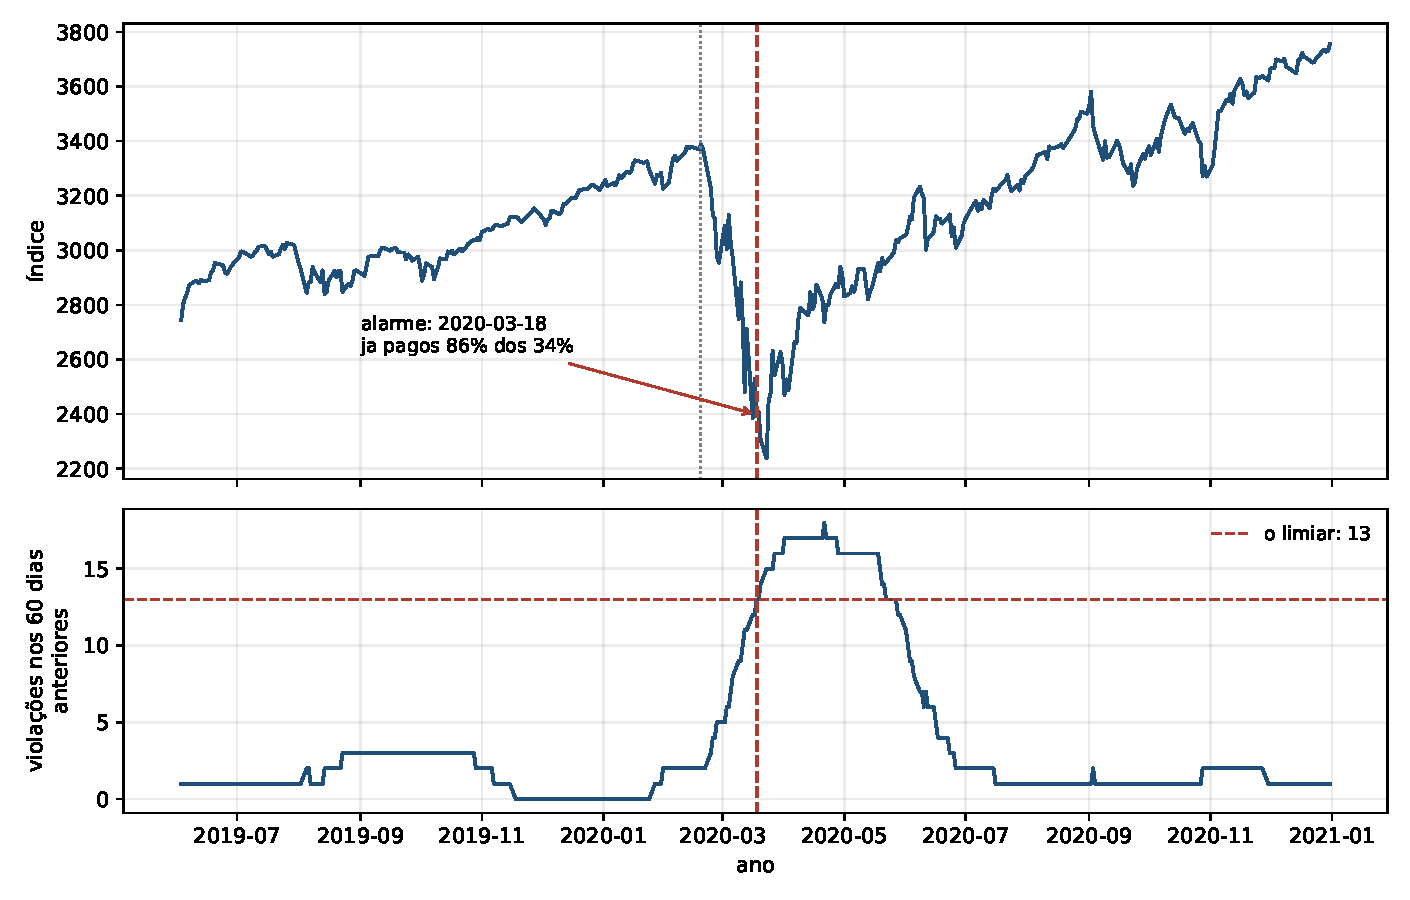
\includegraphics[width=\linewidth]{figuras/E02_orcamento_2.pdf}
  \caption{O alarme de \numVigiaTomboRecenteData{} visto dos dois lados. Em cima, o índice;
    embaixo, as violações dos \numVigiaBloco{} dias anteriores, com o limiar. As duas linhas
    contam a mesma história --- e a de baixo conta depois da de cima.}
  \label{fig:vigia2020}
\end{figure}

\section{O mesmo corte, lido mais fundo}

Tudo o que foi medido até aqui é uma leitura do corte do capítulo anterior: contar quantas
vezes o preço rompeu a linha, e alarmar quando a contagem enche. O corte admite uma segunda
leitura, mais direta, e vale olhá-la antes de aceitar que o vigia é assim mesmo.

Nessa leitura o alarme não espera contagem nenhuma. Ele soa no dia em que o preço fica abaixo
do $k$-ésimo pior dos últimos $n$ dias; com $k = 1$, soa no dia em que o preço faz o pior dia
do último ano. É o mesmo corte, com o posto escolhido de outro jeito, e dessa vez a escolha
tem conta fechada, porque é a proposição do capítulo anterior lida ao contrário: o posto $k$
com janela $n$ assina a taxa $k/(n+1)$.

Isso muda a natureza do orçamento. Na leitura do bloco, a frequência do falso alarme não tem
forma fechada --- sessenta blocos móveis se sobrepõem, e o melhor que se consegue é medir, com
o erro de contagem que a \cref{prop:teto} limita por cima. Na leitura do dia a frequência é
exata, e o número declarado é o número entregue: nos mundos que nunca mudam, a medição
devolveu \numSegundaLeituraParadoAlarmes{} alarmes contra os \numSegundaLeituraParadoDeclarado{}
que a conta declara.

Daí sai um limite que calibração nenhuma contorna. O posto mais fundo possível é o primeiro da
fila, de modo que com $n$ dias de memória --- e aqui \textbf{memória} é o nome do que se compra:
quantos dias o alarme olha para trás --- o alarme mais raro que existe é $1/(n+1)$.
% aterramento: memoria-janela
Um alarme
por ano custa \numMemoriaUmAlarmePorAnoDias{} dias de memória; um alarme por década custa
\numMemoriaUmAlarmePorDecadaDias{} dias, que são dez anos de série, e quem não tem esses dias
não tem esse alarme.

O que essa leitura compra é tempo. No orçamento de \numFundoUmAnoAlarmesPorAno{} alarme por
ano, ela avisou do tombo recente em \numSegundaLeituraTomboRecenteData, com
\numSegundaLeituraTomboRecentePagoPct\% do prejuízo já pago, contra os
\numVigiaTomboRecentePagoPct\% da leitura do bloco. No tombo antigo, avisou em
\numSegundaLeituraTomboAntigoData{} com \numSegundaLeituraTomboAntigoPagoPct\%, contra
\numVigiaTomboAntigoPagoPct\% da outra leitura.

A comparação, porém, pede cuidado, porque os dois vigias foram declarados em orçamentos
diferentes: \numFundoUmAnoAlarmesPorAno{} alarme por ano de um lado, um a cada
\numVigiaAnosParadoPorAlarme{} anos do outro. No ponto em que os dois orçamentos se aproximam,
a vantagem some. Com \numFundoCincoAnosAlarmesPorAno{} alarme por ano, ou um a cada cinco
anos, a leitura do dia chegou ao tombo recente em \numSegundaLeituraCincoAnosTomboRecenteData{}
com \numSegundaLeituraCincoAnosTomboRecentePagoPct\% do prejuízo pago; a leitura do bloco, no
limiar \numTrocaOitoLimiar, soa uma vez a cada \numTrocaOitoAnos{} anos e chega com
\numTrocaOitoPagoPct\%. Duas leituras do mesmo corte, silêncios próximos e quase o mesmo preço.

E a leitura do dia tem um preço próprio, que a tabela do bloco não mostra. Num mundo que nunca
muda ela soa, por construção, na taxa que declarou: a conta pede
\numSegundaLeituraParadoDeclarado{} alarmes e a medição devolveu \numSegundaLeituraParadoAlarmes{}.
Na série real foram \numSegundaLeituraAlarmesReais{}, ou \numSegundaLeituraAlarmesAno{} por ano,
contra o \numFundoUmAnoAlarmesPorAno{} declarado --- enquanto o vigia do bloco soou
\numVigiaAlarmesReais{} vezes no mesmo período. A escolha é entre um vigia que fala \numSegundaLeituraAlarmesAno{}
vezes por ano e chega cedo, e um vigia que fala uma vez a cada três anos e meio e chega depois.

\section{O que fica}

O que fica é o orçamento, e ele fixa uma coisa só: \textbf{todo alarme é um par declarado} ---
com que frequência ele soa quando nada muda, e quanto ele demora quando algo muda. Um alarme que não declara o par não é uma afirmação; é barulho com opinião. Fica também
a moeda do par: ele se compra com memória, porque o alarme mais raro que $n$ dias de janela
permitem é $1/(n+1)$, e se paga conforme a forma da mudança, que decide quantos dias custa
sair do silêncio.

E fica o fracasso seguinte, que a curva da troca não mostra: ela foi medida com os tombos do
mercado, e o tombo é a forma de mudança mais fácil de ver. O mundo muda de outras maneiras.


% O capítulo 5 — volta 1: a forma da mudança decide o preço do silêncio.

\input{capitulos/05_forma_decide_o_preco.tex}

% O capítulo 6 — a segunda forma que a margem não vê: o calendário.

\input{capitulos/06_o_dia_da_semana.tex}

% O capítulo 7 — a última forma da volta 1: a dependência, que não está em margem nenhuma.

\input{capitulos/07_dia_em_que_tudo_cai}

% O capítulo 8 — a volta 2: a estatística que estima não anuncia, e o controle diz por quê.

\input{capitulos/08_estatistica_que_nao_anuncia}

% O capítulo 9 — a volta 3: quantas explicações cabem nos mesmos dados.

\input{capitulos/09_quantas_explicacoes_cabem}

% O capítulo 10 — a volta 4: ver mundos basta, ou é preciso mexer no mundo?

\input{capitulos/10_ver_mundos_basta}

\part{A travessia}

Cada instrumento construído até aqui lê uma margem de uma série, e é isso que a travessia vem
testar. O objeto de uma família passa a ser medido com o instrumento de outra: a dependência com
o vigia da margem, a intervenção com o desenho do experimento, a leitura da série com a partilha
do relógio, e a direção do tempo com o orçamento do alarme. As cinco perguntas pagam em moedas
diferentes --- dias de experimento, trabalho de atualização, passado apagado, anos de espera.

% O capítulo 11 — a travessia: o vigia de margem não vê a dependência.

\input{capitulos/11_vigia_nao_ve}

% O capítulo 12 — a travessia: o que separa duas explicações que a observação empatou.

\input{capitulos/12_desenho_da_intervencao}

% O capítulo 13 — a travessia: proteger e adaptar disputam o mesmo relógio.

\chapter{A partilha do relógio}\label{cap:partilha}

O capítulo da intervenção terminou com uma dívida declarada: se o orçamento é um só, os dias gastos
segurando o mundo para conhecê-lo são dias em que o sistema não aprende nada de novo. A pergunta
que sobra é a da travessia entre proteger e adaptar: \textbf{recalibrar a barreira compete com acompanhar
o mundo?}

\section{A barreira tem dois ingredientes}

A barreira desta travessia é o produto de duas coisas, e as duas não se comportam do mesmo jeito\cite{sebastian2025enhancing}.

\begin{definicao}[escala e forma]\label{def:escala-forma}
A \emph{escala} de um dia é o nível da oscilação, estimado com os dias anteriores a ele. A
\emph{forma} é o corte da série já dividida pela escala: quantas vezes o nível a barreira fica acima
dele. A barreira do dia é o produto da escala pela forma.
\end{definicao}

A escala é a média de \numPartilhaJanelaEscala{} dias, e a forma é o \numPartilhaPosto{}º maior dos
últimos \numPartilhaJanelaForma{} dias padronizados. Os dois números são escolhas declaradas. O que se
mede não depende deles.

A moeda também precisa ser dita antes de ser usada, e é a natural de quem protege: a soma do que
passou por cima da barreira, dia a dia. Uma moeda só, para os dois ingredientes, de modo que comparar
não exige declarar um câmbio entre coisas diferentes.

O defeito que este capítulo mede é o palpite simétrico: tratar proteger e acompanhar como dois
consumidores iguais do mesmo relógio, e repartir o orçamento de atualizações meio a meio.

\section{As duas pressas}

O mundo da medição é uma série de \numPartilhaDiasDeSerie{} dias que dobra a sua oscilação de uma
vez, a um quarto do caminho. A avaliação olha os \numPartilhaHorizonte{} dias seguintes à mudança, em
\numPartilhaSementes{} mundos sorteados, e a dispersão vem junto.

O controle é o mesmo desenho num mundo que não muda: ali a perda absorvida é de
\numPartilhaPisoParado{} por dia, com dispersão de \numPartilhaPisoParadoDispersao{}. É contra esse
piso que as demais contas se leem.

\begin{figure}[htbp]
  \centering
  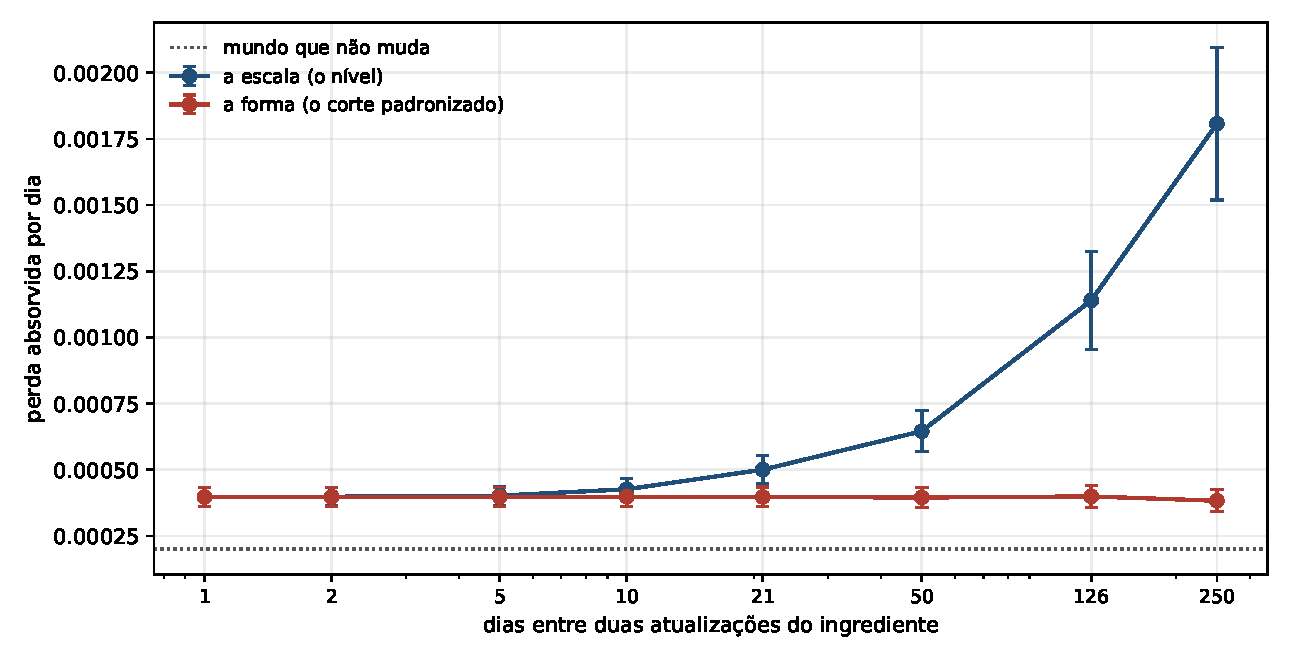
\includegraphics[width=\linewidth]{figuras/E11_partilha_do_relogio_1.pdf}
  \caption{A perda absorvida contra o tempo entre duas atualizações, atualizando um ingrediente por
    vez. O eixo dos tempos é logarítmico, de modo que a distância entre as últimas marcas vale muito
    mais dias do que a figura sugere. A linha pontilhada é o mesmo desenho num mundo que não muda.}
  \label{fig:duas_pressas}
\end{figure}

Atualizar a escala todo dia custa \numPartilhaEscalaDia{} de perda por dia; deixá-la envelhecer
duzentos e cinquenta dias custa \numPartilhaEscalaLenta{}, \numPartilhaRazaoEscala{} vezes o valor de
todo dia. A forma, medida do mesmo jeito, sai de \numPartilhaFormaDia{} para \numPartilhaFormaLenta{} ---
uma razão de \numPartilhaRazaoForma{}. As duas pressas diferem por quase cinco vezes de um lado e
por nada do outro.

A razão disso não é um acidente da medição, e vale escrever a conta que a sustenta.

% aterramento: padronizacao
% aterramento: c
\textbf{Padronizar} é dividir cada dia pela escala daquele dia: o valor padronizado é o afastamento
do dia medido em unidades do tamanho típico de então, e é ele que diz se o dia foi grande ou pequeno
para o mundo daquele momento. A letra $c$ é a constante positiva que multiplica a série inteira até
um instante, e a proposição diz o que acontece com a série padronizada quando o mundo todo cresce de
tamanho.

\begin{proposicao}[a escala some na padronização]\label{prop:padronizacao}
Se a série for multiplicada por uma constante positiva $c$ até o instante $t$, a série padronizada
não muda em nenhum instante até $t$. Em particular o corte da forma é o mesmo, e só a escala
carrega a mudança.
\end{proposicao}

\begin{proof}
A escala estimada em $t$ é a média dos dias anteriores a $t$; multiplicando a série por $c$, essa
média fica multiplicada por $c$. O valor padronizado é a razão entre o dia e a sua escala, de modo
que o $c$ do numerador e o $c$ do denominador se cancelam. O corte é um posto dessa razão, e um
posto não muda quando todos os seus valores são multiplicados pela mesma constante.
\end{proof}

Uma mudança que só multiplica a oscilação é invisível para a forma e é tudo para a escala. Por isso
a forma pode ser atualizada de vez em quando e a escala precisa ser atualizada sempre: cada uma
carrega a parte da mudança que a outra não vê\cite{borkar1997stochastic}.

\section{A partilha}

Com um orçamento de \numPartilhaOrcamento{} atualizações ao longo dos \numPartilhaHorizonte{} dias
de avaliação, a divisão pode ser medida inteira.

\begin{table}[htbp]
  \centering
  \small
  \begin{tabular}{rrr}
    \hline
    fração do orçamento & perda absorvida & \\
    que vai para a escala & por dia & \\
    \hline
    nenhuma & \numPartilhaSemAtualizarEscala & a escala fica velha \\
    metade & \numPartilhaMeioAMeio & o palpite simétrico \\
    \numPartilhaMelhorFracao & \numPartilhaMelhor & o melhor desenho medido \\
    \hline
  \end{tabular}
  \caption{A partilha do orçamento de \numPartilhaOrcamento{} atualizações. O desvio entre os \numPartilhaSementes{} mundos sorteados está na \cref{fig:partilha}. A
    fração que falta em cada linha vai para a forma.}
  \label{tab:partilha}
\end{table}

Deixar a escala sem atualização nenhuma leva a perda a \numPartilhaSemAtualizarEscala{},
\numPartilhaRazaoSemEscalaSobreMelhor{} vezes o valor do melhor desenho. Repartir meio a meio dá
\numPartilhaMeioAMeio{}, e a melhor partilha
medida é a de \numPartilhaMelhorFracao{} do orçamento para a escala, com
\numPartilhaMelhor{} --- \numPartilhaGanhoMeioAMeioPct\% menos perda do que o palpite simétrico, com
o mesmo trabalho.

O melhor ponto medido fica antes do extremo, e a diferença entre ele e dar tudo à escala é pequena ---
pequena o bastante para não se ler sem a dispersão. A partilha certa não é a igualitária nem a extrema\cite{grossberg1987competitive}.

\section{Quando a partilha morde}

Falta o controle que separa o que é do desenho do que é da pobreza do orçamento. Apertando o
orçamento e repetindo a mesma pergunta:

\begin{table}[htbp]
  \centering
  \small
  \begin{tabular}{rrr}
    \hline
    atualizações & perda com quase & ganho sobre o \\
    no horizonte & toda a escala & meio a meio \\
    \hline
    cinco & \numPartilhaQuaseTodaCinco & \numPartilhaGanhoCincoPct\% \\
    vinte & \numPartilhaQuaseTodaVinte & \numPartilhaGanhoVintePct\% \\
    sessenta & \numPartilhaQuaseTodaSessenta & \numPartilhaGanhoSessentaPct\% \\
    duzentos e cinquenta & \numPartilhaQuaseTodaDuzentosECinquenta & \numPartilhaGanhoDuzentosECinquentaPct\% \\
    \hline
  \end{tabular}
  \caption{O ganho de partilhar bem, contra o tamanho do orçamento. Com orçamento folgado, dividir de
    qualquer maneira dá quase o mesmo.}
  \label{tab:aperto}
\end{table}

Com cinco atualizações no horizonte, a partilha de \numPartilhaMelhorFracao{} do orçamento para a escala vale
\numPartilhaGanhoCincoPct\% menos perda do que o palpite simétrico;
perda; com duzentos e cinquenta, vale \numPartilhaGanhoDuzentosECinquentaPct\%. A competição que a
pergunta supõe existe, e aparece no aperto: enquanto houver atualizações de sobra, os dois
ingredientes recebem o que precisam e não disputam nada.

A última conta fecha o sentido do capítulo. Manter os dois ingredientes atualizados todo dia, ao
longo de \numPartilhaSobraAtualizacoes{} dias, leva a perda a \numPartilhaSobra{}, com desvio de
\numPartilhaSobraDispersao{} entre os mundos sorteados. O melhor desenho com \numPartilhaOrcamento{}
atualizações no mesmo horizonte fica em \numPartilhaMelhor{}: \numPartilhaApertoSobreTudoPct\% de
perda a mais, na média. A diferença é pequena e não se repete em todo mundo. Comparados par a par
nos mesmos \numPartilhaSementes{} mundos sorteados, o orçamento apertado entrega mais perda em
\numPartilhaApertoMundosQuePerdemContagem{} deles e menos nos
\numPartilhaApertoMundosQueGanhamContagem{} restantes, porque a diferença entre os dois desenhos
mede \numPartilhaApertoPorMundo{} de perda por dia e o desvio dessa diferença entre os mundos é
\numPartilhaApertoPorMundoDispersao{}, maior que ela. A pergunta que fica não é se vale a pena,
mas quanto se está disposto a pagar por um punhado de perda.

\begin{figure}[htbp]
  \centering
  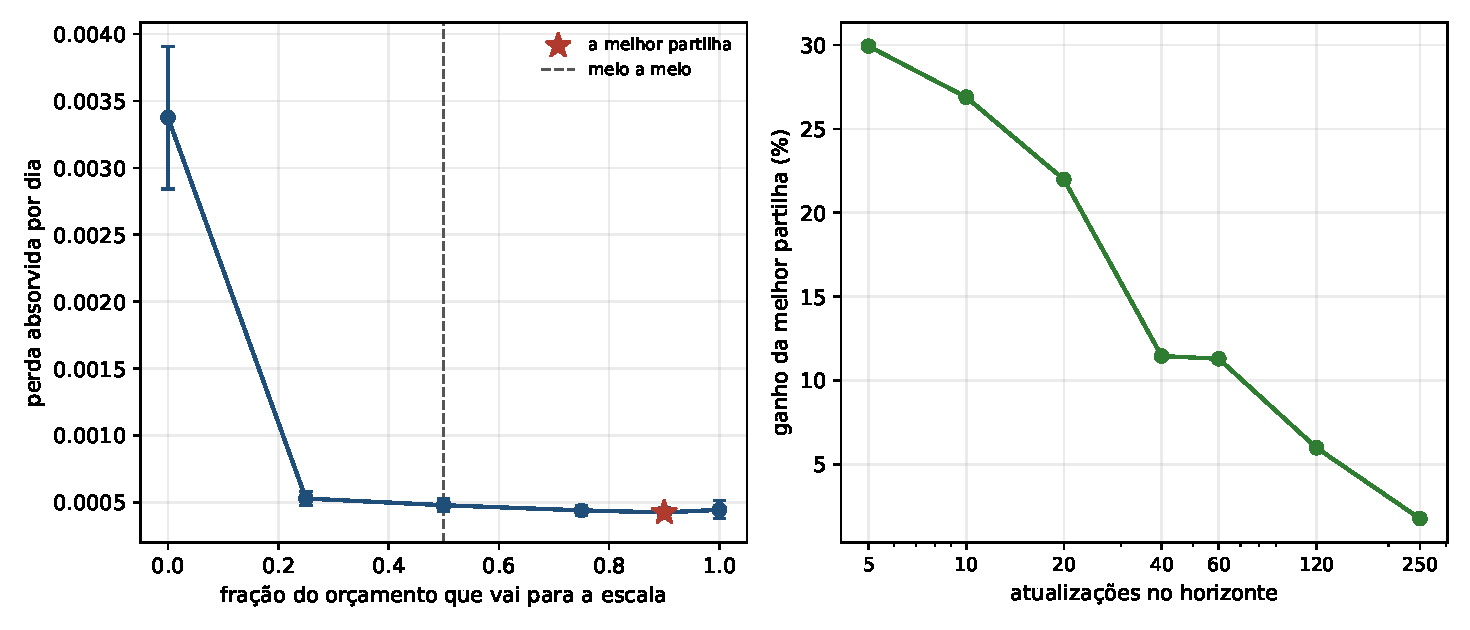
\includegraphics[width=\linewidth]{figuras/E11_partilha_do_relogio_2.pdf}
  \caption{À esquerda, a perda contra a fração do orçamento que vai para a escala, com a dispersão
    entre mundos. O eixo da fração é linear, de modo que os três últimos pontos ficam amontoados à
    direita. À direita, o ganho da melhor
    partilha de \numPartilhaMelhorFracao{} do orçamento para a escala contra o tamanho do orçamento: a
    vantagem de escolher bem encolhe quando o orçamento
    engorda.}
  \label{fig:partilha}
\end{figure}

\section{O que fica}

Fica a resposta da travessia, e ela separa duas coisas que a pergunta juntava. Os dois ingredientes
da barreira não competem pelo dado: o dado é o mesmo fluxo, não se gasta, e cada um pode ter a sua
janela sem tirar nada do outro. O que se gasta é o \textbf{trabalho} de refazer a conta, e aí a
competição é real --- com um desequilíbrio que a proposição explica: a escala carrega tudo o que a
mudança mexeu e a forma não carrega nada, de modo que quase todo o orçamento vai para um lado.

E fica o limite honesto do achado. A competição só morde quando o orçamento é pobre; com
atualizações de sobra, os dois recebem o que precisam e o desenho da partilha deixa de importar.
Isso também é resposta: o refutador declarado da pergunta era um orçamento em que os dois de fato
não competem, e ele existe --- é o orçamento folgado.

O fracasso seguinte está no próprio desequilíbrio que a partilha mediu. A escala é a que precisa ser
atualizada sempre, e atualizar é, no fundo, \textbf{esquecer}: cada atualização troca passado por
presente, e quanto mais depressa a escala acompanha, menos passado ela carrega. Quanto do passado se
pode apagar antes que o sistema deixe de aprender, ninguém mediu ainda, e é essa a próxima conta.


% O capítulo 14 — a travessia: quanto do passado se pode apagar antes de deixar de aprender.

\input{capitulos/14_memoria_que_aprende}

% O capítulo 15 — a travessia: a direção do tempo, com orçamento de alarme.

\input{capitulos/15_vigia_da_direcao}

% O capítulo 16 — a travessia: quem cai primeiro, e se essa ordem se repete.

\chapter{Quem cai primeiro}\label{cap:primeiro}

O capítulo anterior mediu a direção do tempo dentro de uma série. Falta a mesma pergunta no par:
quando as coisas ruins vêm juntas, alguém cai primeiro, e essa ordem se repete?

\section{A ordem que a proteção supõe}

O índice americano e o Ibovespa caem juntos muito mais do que a independência prevê ---
\numConjuntaExcesso{} vezes, medidos nos \numConjuntaDias{} dias em que as duas séries têm corte, com
\numConjuntaRompeA{} rompimentos de um lado, \numConjuntaRompeB{} do outro e \numConjuntaJuntos{} dias
em que os dois rompem ---, e \numConjuntaAcompanhados{} dos rompimentos de uma perna vêm com a outra
no mesmo dia. A leitura
natural de um número desses é que a queda conjunta é um acontecimento só, sem ordem interna: o dia
de uma perna encontra o dia da outra e pronto.

Se for assim, proteger uma perna não ajuda a outra nem atrapalha, porque não há intervalo entre as
duas quedas para fazer nada. A pergunta é se esse intervalo existe.

\section{A contagem}

O instrumento é uma contagem de episódios, e a regra precisa ser dita antes de ser usada.

% aterramento: episodio
\begin{definicao}[episódio dirigido]\label{def:episodio}
Um \emph{episódio} começa no dia em que uma das pernas rompe o próprio corte, desde que nenhum
episódio tenha começado nos \numConjuntaJanelaEpisodio{} dias anteriores --- rompimentos dentro
desses dias não abrem episódio novo. O episódio é \emph{dirigido} quando a outra perna rompe dentro
dos mesmos \numConjuntaJanelaEpisodio{} dias seguintes, e a perna que rompeu primeiro é a
\emph{líder}. A \emph{assimetria} é a diferença entre os episódios liderados por uma perna e os
liderados pela outra, dividida pelo total de episódios dirigidos.
\end{definicao}

Vale um exemplo, porque esta é a única regra do capítulo. Se uma perna rompe num dia e a outra rompe
quatro dias depois, o primeiro rompimento abre o episódio, o segundo o torna dirigido, e a perna que
rompeu primeiro é a líder --- e o segundo rompimento, por cair dentro dos
\numConjuntaJanelaEpisodio{} dias de um episódio que já começou, não abre episódio nenhum.

A regra tem um viés próprio, e escondê-lo seria medir a regra em vez do mundo: a espera olha para
trás e a detecção olha para a frente, de modo que num par sem adiantamento nenhum os dois lados não
saem iguais. Por isso o número do par real só vale contra o número dos pares sorteados, e nunca
contra zero --- é a mesma disciplina dos capítulos do orçamento e da direção.

Pelo mesmo motivo a inversão do relógio não serve de conferência aqui. No capítulo da direção ela
funcionou, porque a estatística de lá não tinha regra nenhuma dentro; aqui a regra é assimétrica, e
virar o mundo ao contrário não a vira junto. Quem confere este instrumento é o nulo, que carrega a
mesma regra.

\section{O nulo, e o par}

Medindo \numConjuntaNulos{} pares sorteados e contemporâneos com a mesma regra, a assimetria tem
média \numConjuntaNuloMedia{} e dispersão \numConjuntaNuloDispersao{}. A média é praticamente zero. Um dia em que as duas caem juntas não tem
primeiro.

Contra esse nulo, o par como veio faz o seguinte.

\begin{table}[htbp]
  \centering
  \small
  \resizebox{\linewidth}{!}{%
\begin{tabular}{rrrr}
    \hline
    janela do & episódios & episódios & assimetria \\
    episódio & liderados pelo índice & liderados pelo Ibovespa & medida \\
    \hline
    um & \numConjuntaLiderAUm & \numConjuntaLiderBUm & \numConjuntaAssimetriaUm \\
    cinco & \numConjuntaLiderACinco & \numConjuntaLiderBCinco & \numConjuntaAssimetriaCinco \\
    dez & \numConjuntaLiderADez & \numConjuntaLiderBDez & \numConjuntaAssimetriaDez \\
    vinte e um & \numConjuntaLiderAVinteEUm & \numConjuntaLiderBVinteEUm & \numConjuntaAssimetriaVinteEUm \\
    \hline
  \end{tabular}}
  \caption{Os episódios dirigidos no par, por janela. A janela é quanto tempo se espera pela
    segunda perna depois de a primeira ter rompido.}
  \label{tab:episodios}
\end{table}

Na janela de \numConjuntaJanelaEpisodio{} dias o índice lidera \numConjuntaLiderA{} episódios e o
Ibovespa lidera \numConjuntaLiderB{}, o que dá uma assimetria de \numConjuntaAssimetria{} ---
\numConjuntaDesvios{} desvios acima do nulo. O número é positivo em todas as janelas testadas, e
não é pequeno.

\section{Quanto dura o adiantamento}

A assimetria diz que existe uma ordem; ela não diz de quanto tempo é o intervalo. Para medir isso, o
instrumento é posto à prova contra um adiantamento declarado: a segunda perna é deslocada dia a dia
e a assimetria é remedida.

\begin{figure}[htbp]
  \centering
  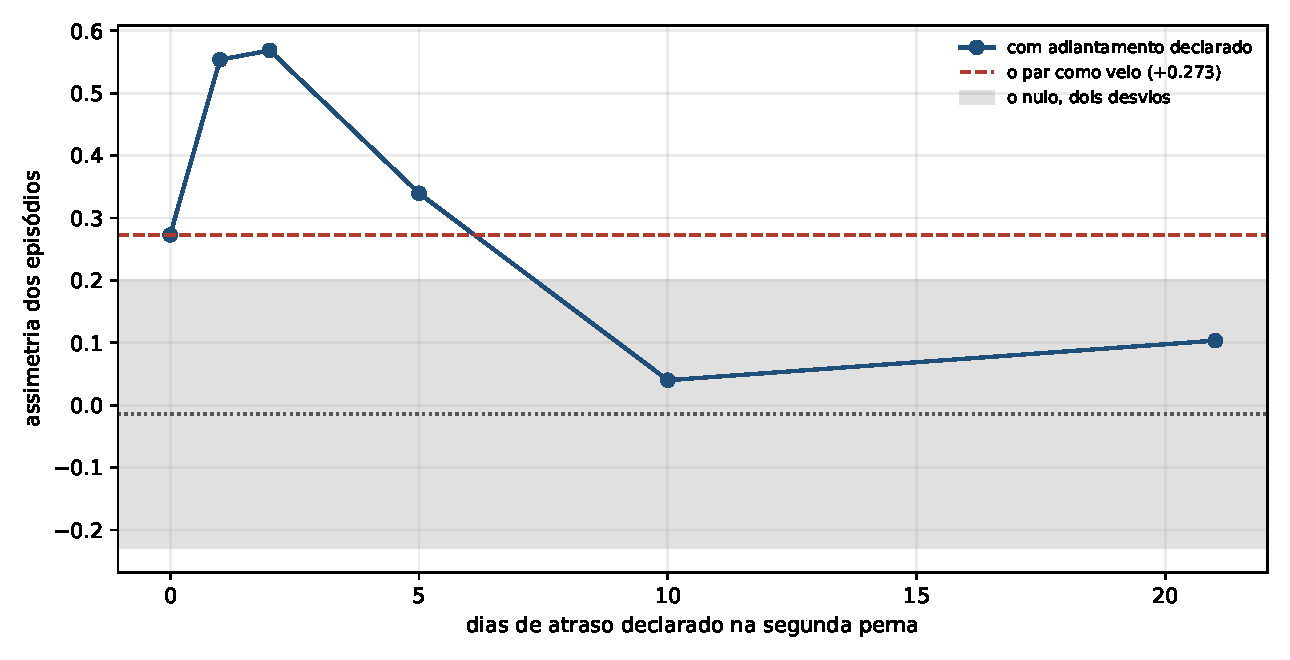
\includegraphics[width=\linewidth]{figuras/E14_direcao_conjunta_1.pdf}
  \caption{A assimetria contra o atraso declarado na segunda perna. A faixa cinza é o nulo a dois
    desvios \emph{sem} deslocamento, a linha tracejada é o par como veio, e a curva é o par com o
    atraso declarado --- que o nulo também sofre, e é o que o texto mede.}
  \label{fig:adiantamento}
\end{figure}

A curva sobe antes de descer. Sem deslocamento nenhum a assimetria é \numConjuntaControleZero{}.
Com a segunda perna deslocada em um ou dois dias, ela chega ao seu máximo ---
\numConjuntaControleUm{} e \numConjuntaControleDois{} ---, acima do valor do par como veio. Com
cinco dias cai para \numConjuntaControleCinco{}, com dez dias para \numConjuntaControleDez{}, e com
\numConjuntaAtrasoMaior{} dias para \numConjuntaControleVinteEUm{}, dentro da faixa do nulo.

Mas o nulo sobe junto, e é isso que a subida mede. Aplicando aos pares sorteados o \emph{mesmo}
deslocamento declarado, a assimetria do nulo no atraso de um dia vale
\numConjuntaNuloDeslocadoUm, contra \numConjuntaNuloDeslocadoZero{} sem deslocamento nenhum: um par
que não tem adiantamento algum pica no mesmo lugar, e o pico é do instrumento.

Vale dizer o que o eixo faz. Os seis pontos estão na posição do atraso que declaram, de modo que o
passo de dez para vinte e um dias ocupa onze vezes a largura do passo de zero para um. O pico cai no
trecho mais estreito do desenho: quem olha a curva de longe vê um tremor no começo da linha, e é ali
que está o achado.

O que a varredura localiza é menos do que a subida sugere. Contra o nulo deslocado, a evidência do
par no atraso zero é de \numConjuntaDesvios{} desvios, e nos atrasos de um e dois dias ela fica da
mesma ordem --- \textbf{o que esta medição sustenta é que existe uma ordem, e num intervalo curto;
ela não separa um dia de dois}. O intervalo curto é o que uma proteção teria entre o rompimento de
uma perna e o da outra, e é ele que decide se há alguma coisa a fazer no meio.

\section{Se repete}

Uma direção medida uma vez é um episódio do dado, e não uma propriedade dele. A conferência é
partir o par em pedaços e medir cada um.

\begin{figure}[htbp]
  \centering
  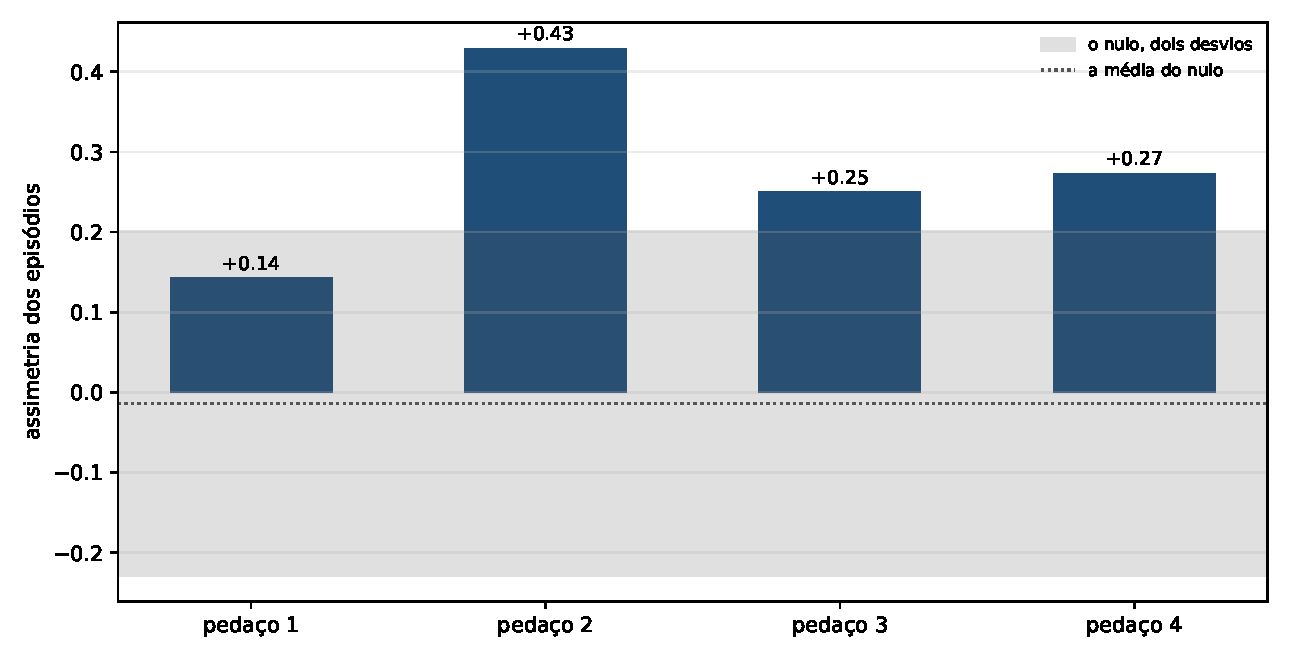
\includegraphics[width=\linewidth]{figuras/E14_direcao_conjunta_2.pdf}
  \caption{A assimetria em cada pedaço do par, contra a faixa do nulo. Os quatro pedaços do par têm
    \numConjuntaPrimeiroDias{}, \numConjuntaSegundoDias{}, \numConjuntaTerceiroDias{} e
    \numConjuntaQuartoDias{} dias de série, e o primeiro perde a janela inicial, em que o corte
    ainda não existe.}
  \label{fig:pedacos}
\end{figure}

Os quatro pedaços dão \numConjuntaPrimeiroAssimetria{}, \numConjuntaSegundoAssimetria{},
\numConjuntaTerceiroAssimetria{} e \numConjuntaQuartoAssimetria{}: todos positivos, e
\numConjuntaPedacosAcima{} de \numConjuntaPedacos{} acima da média do nulo. O sinal se repete --- com
uma ressalva que a régua certa impõe: medida no comprimento de \emph{um} pedaço, a faixa do nulo tem
dispersão de \numConjuntaNuloPedacoDispersao{} e borda de dois desvios em \numConjuntaNuloPedacoBorda,
e nenhum pedaço sozinho a alcança. O que se repete é o sinal, não a evidência de cada pedaço. O
tamanho varia bastante de pedaço para pedaço, e o motivo está na contagem: os quatro pedaços têm
\numConjuntaPrimeiroLiderA{}, \numConjuntaSegundoLiderA{}, \numConjuntaTerceiroLiderA{} e
\numConjuntaQuartoLiderA{} episódios dirigidos liderados pelo índice, e com tão poucos episódios cada
pedaço, sozinho, não distingue nada.

\section{O que fica}

Fica a resposta da travessia, e ela é um sim com medida. A perda conjunta tem direção: o índice cai
primeiro, o Ibovespa vem atrás no intervalo curto que a varredura delimita, e a ordem se repete nos
quatro pedaços do dado. A precisão fica de fora. O efeito é de \numConjuntaDesvios{} desvios sobre o total do
par, cada pedaço isolado é fraco, e a regra de contagem não pode ser conferida pelo relógio
invertido, porque a regra ela mesma tem lado.

Fica também o que a travessia inteira mostrou, olhando para trás. Cinco perguntas medidas com o
instrumento de outra família, e as cinco deram o mesmo tipo de resposta: existe sinal, e o sinal
custa --- em dias de experimento, em trabalho de atualização, em passado apagado, em anos de espera.
Cada capítulo desta travessia terminou com um preço medido, e onde a conta prometeu o que o mundo
não pagou --- como no vigia da direção --- o preço ficou declarado em vez de escondido.

O que sobra é a pergunta que a travessia deixa de pé ao terminar. Quase tudo o que a espiral mediu
até aqui se compra: memória se compra com dias, atualização se compra com trabalho, um experimento
se compra com replicatas. A espiral vira agora para o outro lado da mesma conta, e a pergunta do
movimento seguinte é o que \textbf{não} se compra de jeito nenhum --- começando pela mais dura de todas,
que é o mundo que não foi observado.


\part{O que não se compra}

O orçamento visto pelo avesso. Três coisas ficam fora de qualquer compra: o mundo que não foi
observado, o dia que já foi apagado e o dia em que tudo cai junto. As três são o mesmo movimento
--- um resumo que comprime ---, e o que escapa da compressão é o que decide a conta.

% O capítulo 17 — andar 1: o que não se compra, começando pelo mundo que não foi observado.

\input{capitulos/17_mundo_que_faltou}

% O capítulo 18 — andar 1: o que foi apagado, e se há preço que traga o passado de volta.

\input{capitulos/18_o_que_foi_apagado}

% O capítulo 19 — andar 1: o que a margem não conta.

\chapter{O que a margem deixa de fora}\label{cap:margem}

Este é o último pedaço do andar, e ele junta duas coisas que a espiral encontrou separadas: o vigia
de margem não vê o que acontece \textbf{entre} as pernas, e ler uma série pelo segundo momento é ler
metade dela. A pergunta é quanto custa a metade que fica de fora.

\section{O experimento controlado pelo segundo momento}

Para medir o que a margem não conta é preciso um par de mundos que tenha tudo igual e uma coisa
diferente. A família usada aqui tem a correlação \textbf{declarada}: com probabilidade $p$ as duas pernas
recebem o mesmo choque, de tamanho $f$, e a correlação do corpo é resolvida para que a correlação
total continue valendo \numMargemRho{} em todos os mundos. Nas linhas da tabela, o dois, o cinco e o dez
por cento nomeiam $p$ --- a chance de o choque comum acontecer ---, e o tamanho $f$ é o mesmo nos três:
o mundo do choque grande repete os cinco por cento com um choque maior.
% aterramento: f
O que muda de um mundo para o outro é a forma como os dias ruins chegam juntos --- e também o
tamanho de cada perna, que o choque comum engrossa: a variância da margem sobe de
\numMargemVarianciaMenor{} a \numMargemVarianciaMaior{} entre o controle e o mundo mais grosso.

O controle é o par gaussiano puro, que é o mundo sem choque comum. A família tem \numMargemMundos{} mundos --- o controle e
quatro com o choque declarado ---, medidos em \numMargemDias{} dias e
\numMargemSementes{} sorteios por célula, com o corte na janela de \numMargemJanela{} dias e a
carteira com peso igual, \numMargemPeso{} em cada perna.

Se o segundo momento resumisse o risco conjunto, nada mudaria entre esses mundos.

\section{O que fica parado e o que cresce}

\begin{table}[htbp]
  \centering
  \small
  \resizebox{\linewidth}{!}{%
\begin{tabular}{lrrr}
    \hline
    mundo & correlação & curtose da & dias juntos, \\
    & medida & margem & contra a independência \\
    \hline
    controle & \numMargemCorrelacaoControle & \numMargemCurtoseControle & \numMargemExcessoControle \\
    choque em dois por cento & \numMargemCorrelacaoDoisPorCento & \numMargemCurtoseDoisPorCento & \numMargemExcessoDoisPorCento \\
    choque em cinco por cento & \numMargemCorrelacaoCincoPorCento & \numMargemCurtoseCincoPorCento & \numMargemExcessoCincoPorCento \\
    choque em dez por cento & \numMargemCorrelacaoDezPorCento & \numMargemCurtoseDezPorCento & \numMargemExcessoDezPorCento \\
    choque grande & \numMargemCorrelacaoChoqueGrande & \numMargemCurtoseChoqueGrande & \numMargemExcessoChoqueGrande \\
    \hline
  \end{tabular}}
  \caption{A correlação declarada é respeitada em todos os mundos --- a medida vai de
    \numMargemCorrelacaoMenor{} a \numMargemCorrelacaoMaior{} ---, e o que muda é a cauda e o
    agrupamento dos dias ruins. A última coluna é o instrumento do capítulo da dependência: quantas
    vezes os dois rompem juntos, contra o que a independência preveria.}
  \label{tab:margem}
\end{table}

A correlação anda de \numMargemCorrelacaoMenor{} a \numMargemCorrelacaoMaior{}, um vaivém de menos
de dois por cento que é ruído de amostragem. No mesmo conjunto de mundos, os dias em que as duas
pernas rompem juntas vão de \numMargemExcessoMenor{} a \numMargemExcessoMaior{} vezes o que a
independência preveria: quase o dobro. A \emph{correlação} fica parada enquanto o agrupamento dos dias
ruins quase dobra --- mas o segundo momento não fica: o choque comum engrossa cada perna, e a
variância da margem dobra. Duas contas separam a escala da forma. Padronizando cada perna pela própria
variância antes de medir a perda, a razão entre o pior mundo e o controle cai de \numMargemPerdaRazao{}
para \numMargemPerdaPadraoRazao. E uma gaussiana com a variância e a correlação de cada mundo --- sem
cauda nenhuma --- já entrega \numMargemPerdaGaussianaRazao{} dessa razão: \textbf{a maior parte do que
a perda conjunta cresce é a margem que o choque engrossou}, e o que sobra para a forma é a parte
pequena, que é a que este capítulo persegue.

\begin{table}[htbp]
  \centering
  \small
  \begin{tabular}{lrr}
    \hline
    mundo & perda conjunta & além do próprio \\
    & no pior \numMargemCauda{} & corte \\
    \hline
    controle & \numMargemPerdaControle & \numMargemProfundidadeControle \\
    choque em dois por cento & \numMargemPerdaDoisPorCento & \numMargemProfundidadeDoisPorCento \\
    choque em cinco por cento & \numMargemPerdaCincoPorCento & \numMargemProfundidadeCincoPorCento \\
    choque em dez por cento & \numMargemPerdaDezPorCento & \numMargemProfundidadeDezPorCento \\
    choque grande & \numMargemPerdaChoqueGrande & \numMargemProfundidadeChoqueGrande \\
    \hline
  \end{tabular}
  \caption{A perda média de uma carteira de peso igual no pior \numMargemCauda{} dos dias, e a
    profundidade média além do corte de uma das pernas. A coluna da perda é o prejuízo; a de além do corte é
    o que a margem paga quando ele é rompido.}
  \label{tab:perdas}
\end{table}

A perda conjunta sai de \numMargemPerdaMenor{} para \numMargemPerdaMaior{}, uma razão de
\numMargemPerdaRazao{} entre o mundo mais calmo e o mais pesado, sem que a correlação tenha se
mexido. Quem dimensiona a proteção pela correlação dimensiona o mesmo número para os cinco mundos, e
o que se paga no pior dia difere por mais da metade.

\begin{figure}[htbp]
  \centering
  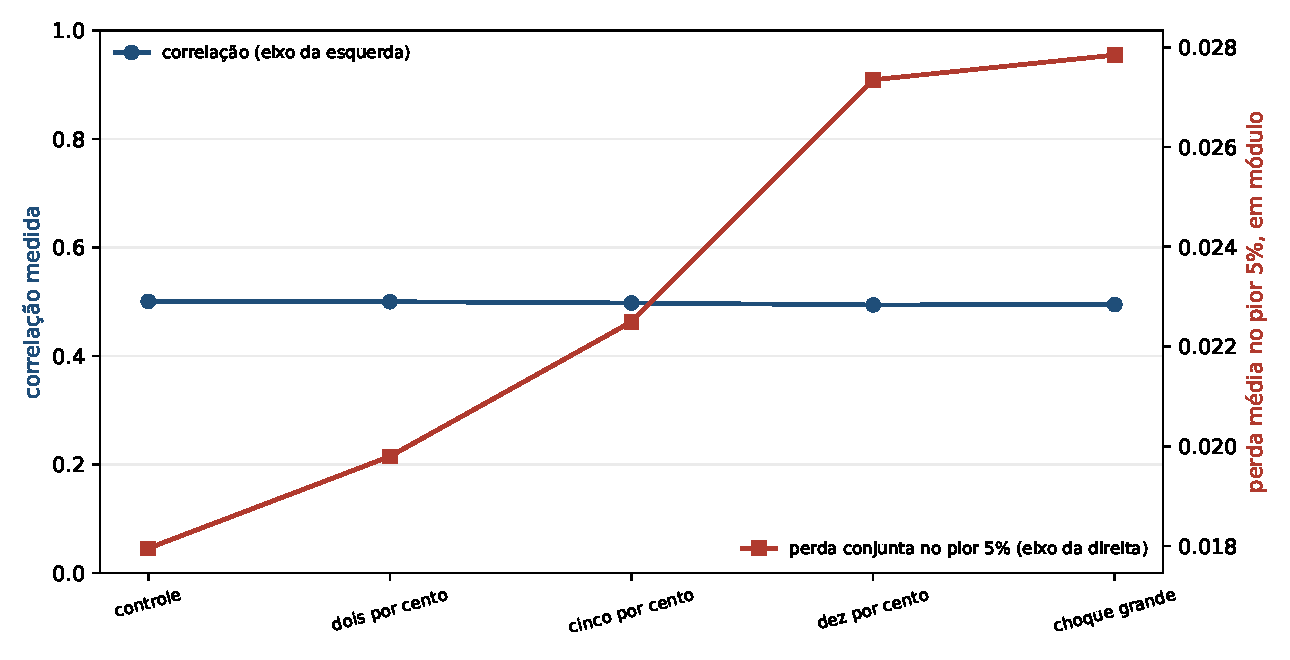
\includegraphics[width=\linewidth]{figuras/E17_o_que_a_margem_nao_conta_1.pdf}
  \caption{A correlação medida e a perda conjunta, contra os cinco mundos. Os dois eixos são
    diferentes de propósito, e as duas linhas se cruzam no meio do caminho: a reta é a correlação, que
    anda de \numMargemCorrelacaoMenor{} a \numMargemCorrelacaoMaior{}, e a que sobe é a perda, que
    começa abaixo dela e termina acima.}
  \label{fig:parado}
\end{figure}

\section{A margem cumpre a taxa e paga mais fundo}

Vale ser exato sobre o que a margem conta e o que ela não conta, porque a diferença é fina e importa.

A taxa de rompimento do corte é \numMargemTaxaDeRompimento{}, na média dos cinco mundos, e o motivo é do
instrumento: o corte é um quantil, e um quantil entrega a taxa que promete em qualquer mundo que tenha
uma distribuição contínua. A promessa do corte é honrada em todos eles.

O que não é honrado é o que acontece \textbf{depois} do rompimento. A profundidade média além do corte vai
de \numMargemProfundidadeControle{} no controle a \numMargemProfundidadeChoqueGrande{} no mundo de
choque grande: o dia em que o corte é rompido passa a doer três vezes e meia mais, e o número de dias não
mudou.
% aterramento: curtose
A curtose é a média da quarta potência da série depois de ela ter sido posta na própria unidade, e
vale três no mundo normal:
quanto maior, mais peso na cauda. A margem conta que a cauda engordou --- a curtose dela vai de \numMargemCurtoseMenor{} a
\numMargemCurtoseMaior{}, e isso é visível numa série só. O que ela não conta é que os dias
engordaram \textbf{juntos}.

\begin{figure}[htbp]
  \centering
  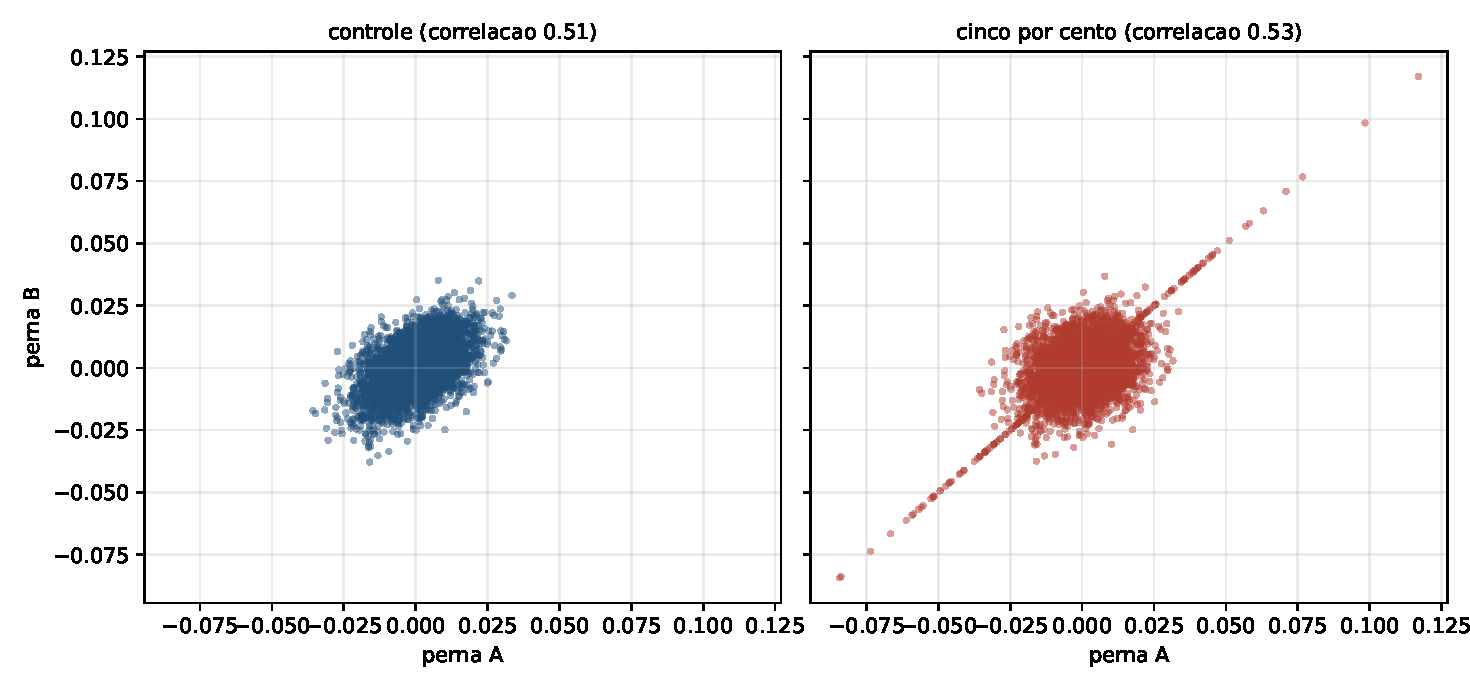
\includegraphics[width=\linewidth]{figuras/E17_o_que_a_margem_nao_conta_2.pdf}
  \caption{A nuvem das duas pernas no mundo gaussiano e no mundo com choque comum. O miolo se abre
    para que a correlação do conjunto continue a mesma, e o que o segundo tem a mais são dois braços
    na diagonal, um para cada canto.}
  \label{fig:nuvem-do-choque}
\end{figure}

Os braços são poucos pontos e ficam fora do corpo da nuvem, além da caixa em que quase todos os
pontos vivem. Um recorte na altura do miolo, que é o corte natural de quem desenha o que é comum,
apagaria exatamente o que o mundo do choque tem a mais.

A figura mostra a diferença de forma, e ela é a coisa toda. Nos dois mundos o miolo é quase a mesma
elipse, e é ele que teve de se abrir para que a correlação do conjunto continuasse em \numMargemRho{}.
O que o mundo do choque tem a mais são dois braços na diagonal, que saem do miolo e vão até os
cantos do gráfico, um para cima e outro para baixo: são os dias em que as duas pernas se movem
juntas e fundo, porque o choque comum tem sinal sorteado, e é no braço de baixo que o prejuízo mora.

\section{O que fica}

Fica a resposta do terceiro pedaço do andar, e ela é mais fina do que a queixa usual contra a
correlação \cite{koike2026measuring}. A margem \textbf{não} é cega à cauda: ela conta que a cauda engordou, e conta pela taxa e pela
profundidade. O que ela não conta é a \textbf{junto}; e como o prejuízo de uma carteira é feito de dias em
que tudo cai ao mesmo tempo, é justamente a parte que falta que decide a conta.

Fica também, com este capítulo, o andar inteiro medido. Os três pedaços são o mesmo movimento visto
de três lugares: o resumo --- o recorde, o estado guardado, o segundo momento --- é sempre uma
compressão, e o que escapa da compressão é exatamente o que decide. O mundo que faltou não está no
recorde, o dia apagado não está no estado, e o dia em que tudo cai junto não está na correlação.

A espiral vira agora para o andar do enquadramento. Tudo o que a espiral mediu até aqui supôs que
havia uma série, um agora e um sistema com fronteira --- e nenhuma dessas três coisas foi discutida.
Elas vêm a seguir, e vêm porque a conta deste andar mostrou quanto custa o que fica de fora quando a
fronteira é escolhida no escuro.


\part{O enquadramento}

A espiral mediu tudo isso supondo três coisas que nunca discutiu: que existe uma série com
começo e fim, que a decisão usa o dado de hoje, e que se sabe quanto passado ainda conta. As
três são escolhas do instrumento, e as três têm preço medido.

% O capítulo 20 — andar 2: o enquadramento, começando pela série.

\input{capitulos/20_o_pedaco_escolhido}

% O capítulo 21 — andar 2: o agora, e as três bordas do enquadramento.

\chapter{O agora}\label{cap:agora}

O capítulo anterior mediu o corte no espaço: onde a série começa e termina. Este mede o corte no
\textbf{tempo}. Há um instante em que a decisão é tomada, e os dados em que ela se apoia são de antes
disso; a distância entre os dois é o atraso, e quase ninguém o declara.

\section{O dado que chega velho}

O atraso entra no corte de um jeito simples: a barreira que vale hoje é a que
foi calculada com o dado de \emph{d} dias atrás, sobre a janela de \numAgoraJanela{} dias. Com \emph{d} zero isso é exatamente o corte, e a identidade vale por construção --- o atraso não muda o instrumento, muda a idade do dado que ele lê.

Medida no índice, nos \numEntregaDias{} dias em que havia janela suficiente dentro dos \numAgoraDias{}
pregões da série --- um dia menos para cada dia de atraso ---, a entrega do corte é esta.

\begin{table}[htbp]
  \centering
  \small
  \begin{tabular}{rrr}
    \hline
    atraso do & entrega & em razão da \\
    dado (dias) & medida & conta do corte \\
    \hline
    nenhum & \numAgoraEntregaZero & \numAgoraRazaoZero \\
    um & \numAgoraEntregaUm & \numAgoraRazaoUm \\
    cinco & \numAgoraEntregaCinco & \numAgoraRazaoCinco \\
    vinte e um & \numAgoraEntregaVinteEUm & \numAgoraRazaoVinteEUm \\
    sessenta e três & \numAgoraEntregaSessentaETres & \numAgoraRazaoSessentaETres \\
    duzentos e cinquenta e dois & \numAgoraEntregaDuzentosECinquentaEDois & \numAgoraRazaoDuzentosECinquentaEDois \\
    \hline
  \end{tabular}
  \caption{A entrega do corte contra a idade do dado, no índice. A conta do corte é de
    \numAgoraPromessa{}, e é ela que a última coluna toma por referência.}
  \label{tab:atraso-do-dado}
\end{table}

Um dia de atraso não se nota. Um ano de atraso entrega \numAgoraRazaoDuzentosECinquentaEDois{} vezes a conta do
corte: o instrumento passa a romper \numAgoraEntregaDuzentosECinquentaEDois{} dos dias onde a conta
pede \numAgoraPromessa{}. E o atraso, na prática, nunca é zero: o dado fecha depois do dia que
descreve, e o intervalo entre o fechamento e a decisão é uma escolha de quem opera.

\section{O atraso não custa dias}

A tentação é ler a tabela acima como um preço por dia de atraso. Não é, e o motivo é aritmético.

\begin{proposicao}[o atraso não cobra dias]\label{prop:atraso-parado}
Num mundo cuja lei não muda no tempo e cujos dias são trocáveis, a entrega do corte não depende do
atraso: para qualquer $d$, a chance de o dia de hoje romper uma barreira erguida sobre os $n$ dias
que terminam $d$ dias antes é a mesma.
\end{proposicao}

\begin{proof}
A barreira de hoje é o $k$-ésimo pior daqueles $n$ dias, e o dia julgado é o de hoje, de modo que
a pergunta é sobre o posto de um dia entre $n+1$. Sob permutabilidade os $n+1$ dias são trocáveis,
o posto do dia de hoje é uniforme entre eles, e a chance de ele estar entre os $k$ piores é
$k/(n+1)$ --- a \cref{prop:conta}, para todo $d$. O atraso desloca a janela no tempo, e a troca de
$d$ não muda a lei de nenhum dos $n+1$ dias.
\end{proof}

É o que a medição do controle encontra. No mesmo experimento em \numAgoraSementes{} mundos que
\textbf{não} mudam, a entrega do corte com atraso de nenhum dia a \numAgoraAtrasoMaior{} dias fica
entre \numAgoraParadoMenor{} e \numAgoraParadoMaior{} --- uma variação de \numAgoraParadoVariacao{}
entre o atraso nenhum e o de um ano, que é o tamanho do ruído contra a proposição. O atraso de um
ano move a taxa no quarto decimal: \numAgoraParadoZero{} no atraso nenhum,
\numAgoraParadoVinteEUm{} em vinte e um dias e \numAgoraParadoMaior{} com um ano.

O que a proposição supõe é o que o mundo que muda quebra, e ali a barreira de ontem já mede outra
coisa. \textbf{O atraso não cobra dias; ele cobra a mudança que coube dentro dele.}

\section{O que ele cobra, então}

Para ver a cobrança é preciso olhar onde o mundo muda. O mundo que muda dobra de uma vez no meio
da série, e a leitura é feita só na janela que segue a mudança --- os \numAgoraHorizonte{} dias
seguintes.

\begin{figure}[htbp]
  \centering
  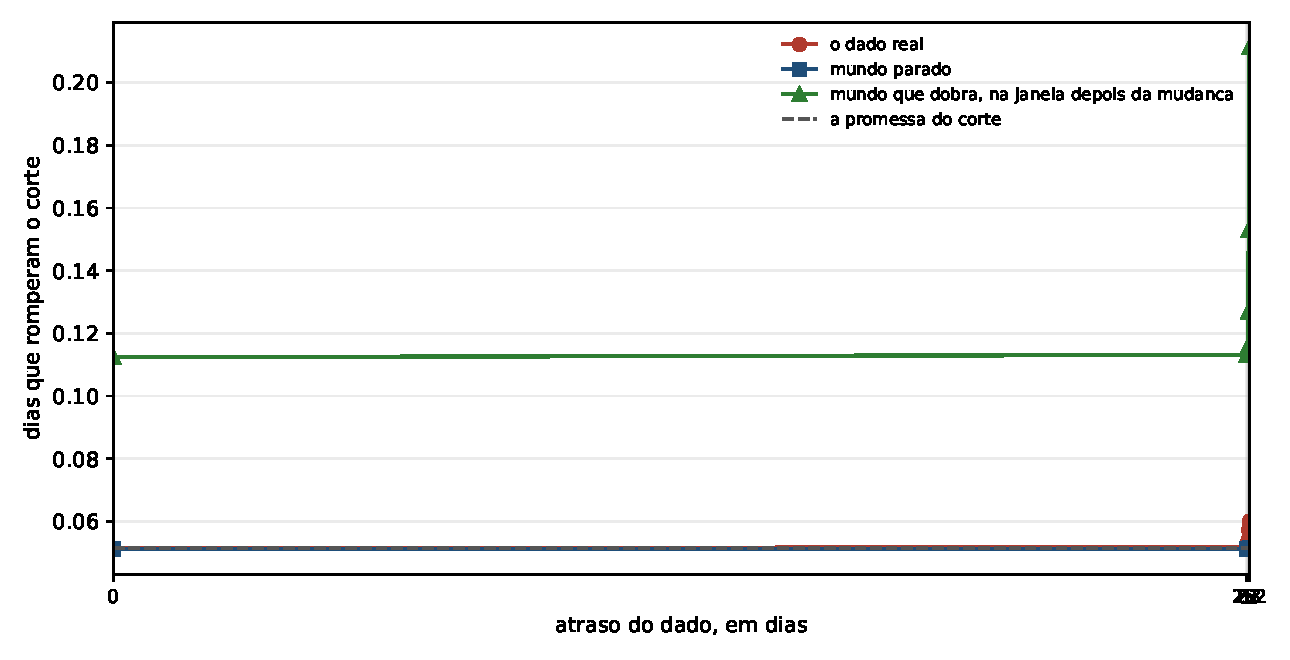
\includegraphics[width=\linewidth]{figuras/E19_o_agora_1.pdf}
  \caption{A entrega do corte contra a idade do dado, nas três situações: o dado real, o mundo que
    não muda e a janela que segue uma mudança. As duas de baixo ficam em cima da promessa em
    qualquer atraso; a de cima é a que segue a mudança.}
  \label{fig:atraso-geral}
\end{figure}

A curva de cima obriga a escala a subir, e as duas linhas de baixo ficam empilhadas na base do
quadro, quase indistinguíveis uma da outra na escala do desenho: quem lê a figura pela impressão
vê a mudança e não vê o atraso.
--- o atraso está nos números.

Na janela depois da mudança, e sem atraso nenhum, a entrega já é de \numAgoraDepoisZero{} --- mais que o dobro
da promessa, e isso é a mudança, não o atraso. Com um ano de atraso ela vai a
\numAgoraDepoisDuzentosECinquentaEDois{}, quatro vezes o prometido.

O que a figura mostra é que as duas coisas se multiplicam. A mudança sozinha já estraga a entrega; o
atraso impede o instrumento de reagir a ela, e o efeito de um sobre o outro é o produto. Num mundo
parado o atraso não aparece; num mundo que muda ele é o que decide quanto tempo a barreira continua
errada.

\begin{figure}[htbp]
  \centering
  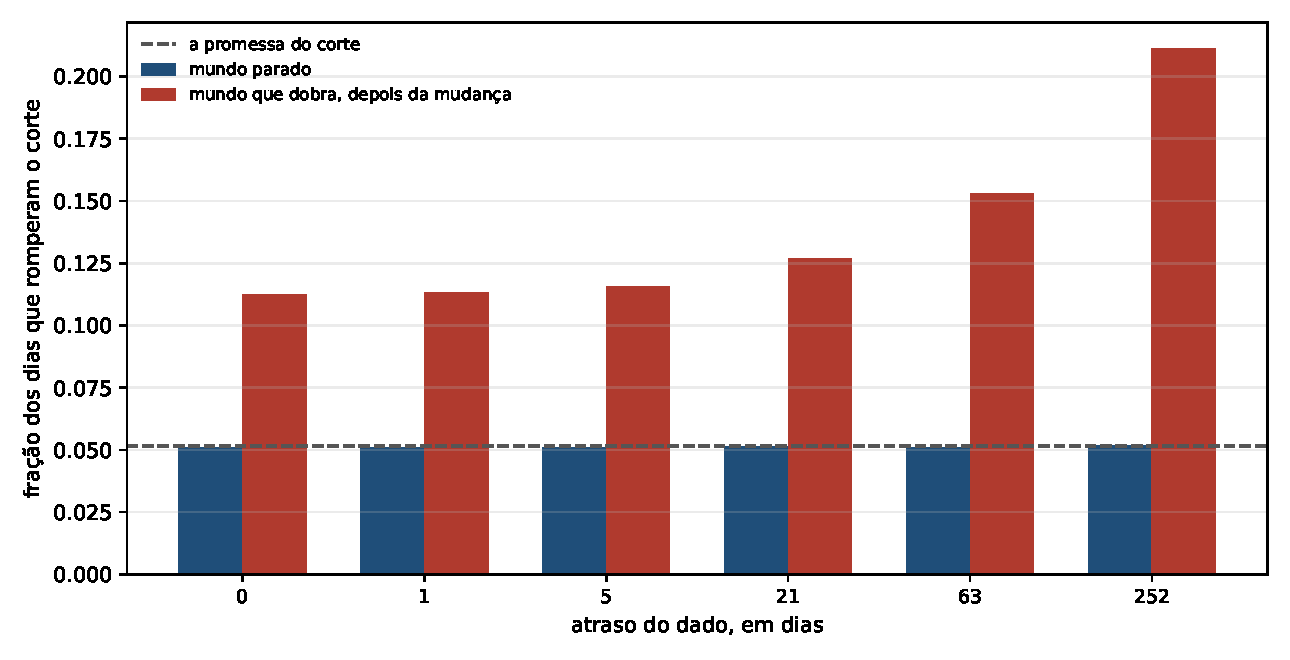
\includegraphics[width=\linewidth]{figuras/E19_o_agora_2.pdf}
  \caption{O mundo parado e o mundo que dobra, por atraso --- o parado medido na série inteira e o
    que dobra na janela que segue a mudança. A barra azul é o controle: ela fica na promessa em
    todos os atrasos.}
  \label{fig:atraso-por-mundo}
\end{figure}

\section{O agora é uma janela}

Com este capítulo o enquadramento fecha, e ele fecha numa imagem só. No instante da decisão --- chamado $t$ ---, o que
um sistema tem é um \textbf{retângulo}: o eixo do tempo vai de $t$ menos o atraso menos a memória até
$t$ menos o atraso. Com atraso nenhum a borda da direita encosta no agora, e o retângulo é o do
capítulo da memória.

A borda da direita é o atraso, medido aqui. A borda da esquerda é a memória, medida duas vezes neste
livro: pela taxa de esquecimento, que diz quanto do passado ainda pesa, e pelo horizonte de
recuperação, que diz até onde o passado apagado volta. E o capítulo anterior mostrou que o próprio
eixo --- onde a série começa e termina --- também é uma escolha.

Nenhuma das três bordas é um fato sobre o mundo. As três são declarações do instrumento, e as três
foram medidas: a individuação, o atraso e a memória. O que sobra depois delas é a pergunta da raiz,
agora com preço conhecido.

\section{O que fica}

Fica a regra do andar do enquadramento, e ela vale para qualquer medição futura: \textbf{declarar as três
bordas}. Onde a série começa e termina, quanto tempo o dado tem, e quanto passado ainda conta.
Nenhuma delas é neutra, e as três foram medidas separadamente neste livro --- com a mesma conclusão
nos três casos, que é a conclusão do livro inteiro: a borda escolhida não é a resposta, e o que
aparece quando ela se mexe é o que ela escondia.

A espiral tem um movimento só por fazer, e ele reaproveita tudo o que já está construído: refazer a pergunta da
raiz. O corte, o orçamento do alarme, a
geometria, a dependência, o esquecimento e o enquadramento já foram medidos; falta lê-los juntos e
responder, com número, o que se pode garantir, medir e otimizar quando o mundo não para de mudar.


\part{O fecho}

A pergunta da raiz, refeita com os buracos abertos ao mesmo tempo: a janela da calibração, o
atraso do dado e o mundo que muda. O que se prometeu no primeiro capítulo é conferido contra o
que se paga, e o preço sai declarado.

% O capítulo 22 — o fecho: a pergunta da raiz, refeita com tudo o que foi construído.

\chapter{O fecho: a promessa com os buracos abertos}\label{cap:fecho}

Dezenove capítulos mediram buracos separados: a memória que cega, o atraso do dado, o pedaço
escolhido, a mudança que chega sem avisar, a cauda que vem junto, o passado que não volta, o trabalho
que se gasta. Cada um tem o seu preço medido, e nenhum foi medido junto com os outros.

Este capítulo mede a promessa do primeiro capítulo com \textbf{três buracos abertos ao mesmo tempo}: a
janela da calibração, o atraso do dado e o mundo. A promessa é a mesma em todas as
\numFechoConfiguracoes{} configurações --- \numPromessaPct{}\% dos dias rompendo o corte, que é
\numFechoPromessa{} em fração ---, com \numFechoJanelas{} tamanhos de
janela em mundos de \numFechoDias{} dias. O posto acompanha a janela, mas ele é um número inteiro:
arredondado para cima, o corte assina sozinho \numFechoAssinadoCurta{} na janela curta,
\numFechoAssinadoMedia{} na média e \numFechoAssinadoLonga{} na longa. A pergunta é se os buracos somam ou se compõem.

\section{A medição da pilha}

\begin{table}[htbp]
  \centering
  \small
  \begin{tabular}{lrrrr}
    \hline
    mundo & janela & atraso & entrega & em vezes \\
    & (dias) & (dias) & medida & a promessa \\
    \hline
    parado & \numFechoJanelaCurta{} & nenhum & \numFechoEntregaParadoCurtaSemAtraso & \numFechoParadoCurtaSemAtraso \\
    parado & \numFechoJanelaCurta{} & \numFechoAtraso{} & \numFechoEntregaParadoCurtaComAtraso & \numFechoParadoCurtaComAtraso \\
    parado & \numFechoJanelaMedia{} & nenhum & \numFechoEntregaParadoMediaSemAtraso & \numFechoParadoMediaSemAtraso \\
    parado & \numFechoJanelaMedia{} & \numFechoAtraso{} & \numFechoEntregaParadoMediaComAtraso & \numFechoParadoMediaComAtraso \\
    parado & \numFechoJanelaLonga{} & nenhum & \numFechoEntregaParadoLongaSemAtraso & \numFechoParadoLongaSemAtraso \\
    parado & \numFechoJanelaLonga{} & \numFechoAtraso{} & \numFechoEntregaParadoLongaComAtraso & \numFechoParadoLongaComAtraso \\
    mudado & \numFechoJanelaCurta{} & nenhum & \numFechoEntregaMudadoCurtaSemAtraso & \numFechoMudadoCurtaSemAtraso \\
    mudado & \numFechoJanelaCurta{} & \numFechoAtraso{} & \numFechoEntregaMudadoCurtaComAtraso & \numFechoMudadoCurtaComAtraso \\
    mudado & \numFechoJanelaMedia{} & nenhum & \numFechoEntregaMudadoMediaSemAtraso & \numFechoMudadoMediaSemAtraso \\
    mudado & \numFechoJanelaMedia{} & \numFechoAtraso{} & \numFechoEntregaMudadoMediaComAtraso & \numFechoMudadoMediaComAtraso \\
    mudado & \numFechoJanelaLonga{} & nenhum & \numFechoEntregaMudadoLongaSemAtraso & \numFechoMudadoLongaSemAtraso \\
    mudado & \numFechoJanelaLonga{} & \numFechoAtraso{} & \numFechoEntregaMudadoLongaComAtraso & \numFechoMudadoLongaComAtraso \\
    \hline
  \end{tabular}
  \caption{A promessa medida nas \numFechoConfiguracoes{} configurações, em
    \numFechoSementes{} mundos sorteados por célula, na janela de \numFechoHorizonte{} dias que segue
    a mudança. A última coluna é a entrega dividida pela promessa, e a dispersão entre os mundos,
    no mundo parado e sem atraso, é de \numFechoDispersaoParadoCurtaSemAtraso{} na janela curta e de
    \numFechoDispersaoParadoLongaSemAtraso{} na longa.}
  \label{tab:pilha}
\end{table}

A primeira metade da tabela traz o mundo parado, e ali a lição é conhecida: \textbf{o que se quer é
entregar a promessa}, e a mais perto dela é a melhor --- a janela longa entrega
\numFechoParadoLongaSemAtraso{} vezes a promessa e a curta \numFechoParadoCurtaSemAtraso{}. A diferença
entre as duas, medida nos mesmos \numFechoSementes{} mundos sorteados, é de \numFechoParadoDiferenca{}
vezes, ou \numFechoParadoDiferencaDesvios{} erros-padrão da média, com dispersão de
\numFechoParadoDiferencaDispersao{} entre os mundos: é o limite do que \numFechoSementes{} mundos
separam. O atraso não move nada de importante.

A segunda metade inverte a ordem. Com o mundo dobrando, a janela longa entrega
\numFechoMudadoLongaSemAtraso{} vezes a promessa e a curta \numFechoMudadoCurtaSemAtraso{}: \textbf{a
memória que era melhor no mundo parado é a pior no mundo que mudou}. O motivo é o mesmo de sempre
--- a janela longa carrega mais dias de antes da mudança, e é por isso que ela demora mais para
esquecer o mundo que já não existe.

\begin{figure}[htbp]
  \centering
  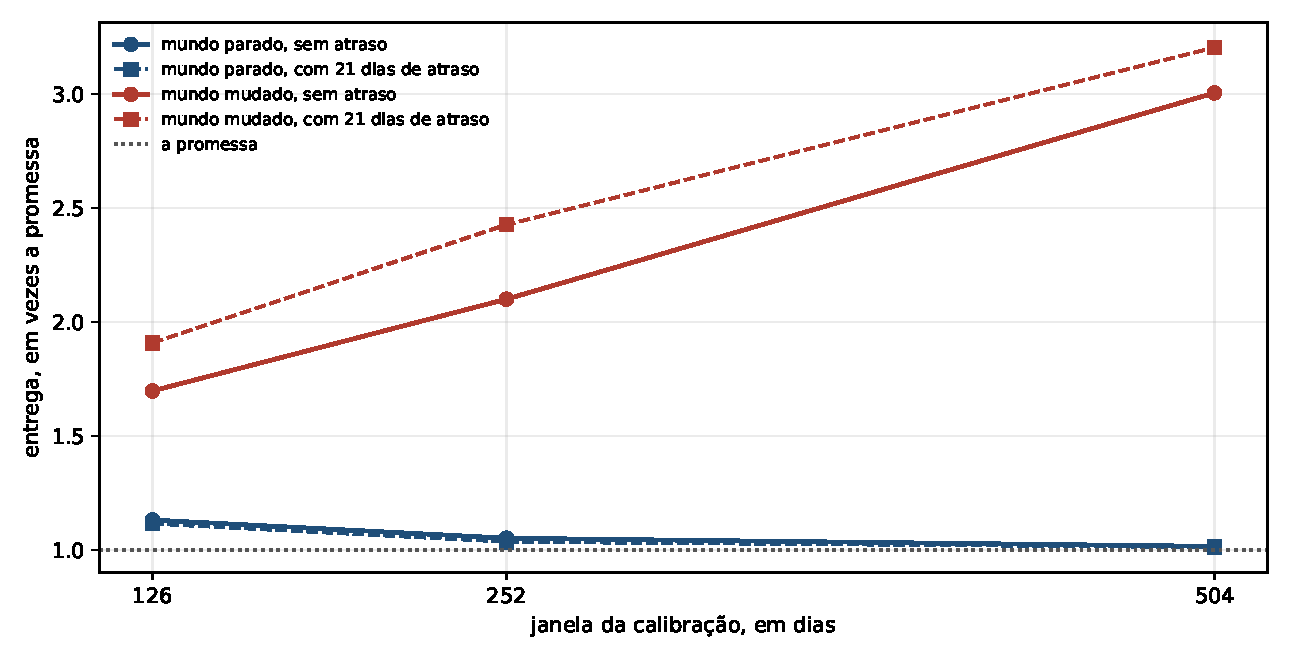
\includegraphics[width=\linewidth]{figuras/E20_o_fecho_1.pdf}
  \caption{A entrega contra a janela da calibração, nos dois mundos e com e sem atraso. As duas
    curvas do mundo parado descem e as duas do mundo que muda sobem: o mesmo eixo, o sentido
    trocado.}
  \label{fig:cruzamento}
\end{figure}

O cruzamento é a coisa toda do capítulo. Num mundo que não muda, aumentar a memória melhora a
entrega; num mundo que muda, aumentar a memória piora. E o sinal do efeito depende de uma coisa que
o instrumento só descobre depois: se o mundo vai mudar.

\section{Os buracos se compõem}

Falta a conta que o título promete. Cada buraco foi medido sozinho, no mundo parado e contra a
mesma promessa: a janela longa entrega \numFechoSoJanelaParado{} vezes a promessa num mundo parado e
\numFechoSoJanelaMudado{} num mundo que muda, o atraso de
\numFechoAtraso{} dias entrega \numFechoSoAtrasoParado{}, e a mudança sozinha entrega
\numFechoSoMudanca{}.

A conta que soma os buracos um a um toma a promessa e acrescenta, a cada vez, o que um buraco sozinho
põe por cima dela --- os incrementos das três barras isoladas da \cref{fig:pilha}. Ela dá
\numFechoSomaIsolada{} vezes, e a pilha passa disso. A pilha inteira --- janela
longa, atraso e mundo que muda, os três juntos --- entrega \numFechoPilha{} vezes a promessa.

A pilha é pior do que a soma dos seus buracos, e é pior por um motivo que o livro encontrou em cada
volta: os buracos não são independentes. A janela longa é inofensiva num mundo que não muda e
devastadora num mundo que muda; o atraso é inofensivo quando a barreira está certa e caro quando ela
está errada; e a mudança é o que transforma os outros dois em dano. É a mesma estrutura da promessa
do primeiro capítulo, agora no instrumento inteiro: o que se paga não é a soma dos defeitos, é o que
eles fazem \textbf{juntos}.

\begin{figure}[htbp]
  \centering
  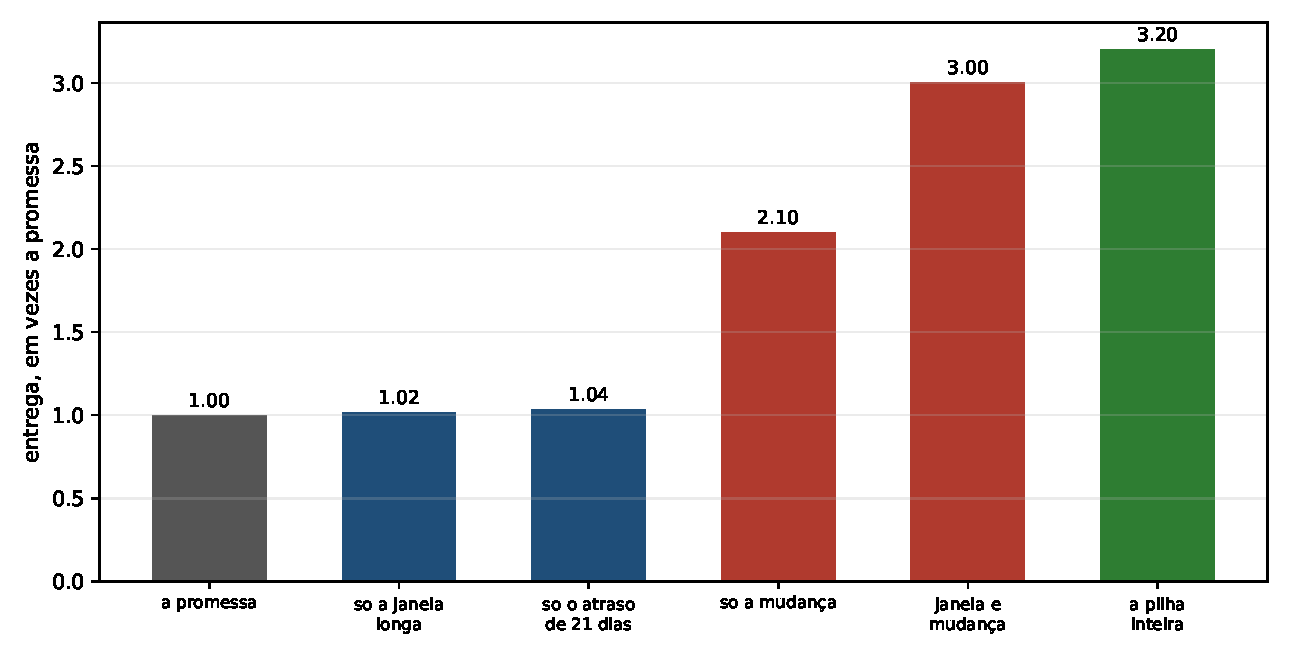
\includegraphics[width=\linewidth]{figuras/E20_o_fecho_2.pdf}
  \caption{A entrega de cada buraco sozinho e a da pilha inteira, em vezes a promessa. A barra verde é a
    mais alta das seis, e o que essa altura diz é o que o livro inteiro perseguiu: os buracos não se
    somam, eles se encaixam.}
  \label{fig:pilha}
\end{figure}

\section{O balanço}

O livro mediu preços em moedas diferentes, e vale olhar para eles na mesma página, cada um na sua.

\begin{table}[htbp]
  \centering
  \small
  \begin{tabular}{lll}
    \hline
    o que foi medido & o número & a moeda \\
    \hline
    a promessa do corte & \numPromessaPct{}\% dos dias & a fração \\
    o orçamento do alarme, no limiar \numVigiaLimiar{} & \numTrocaTrezeAnos{} anos por alarme falso & o tempo de mundo \\
    o que ele paga no tombo & \numTrocaTrezePagoPct{}\% do prejuízo & o prejuízo \\
    a memória que aprende & \numEsquecimentoMelhorMemoria{} dias, erro \numEsquecimentoMelhor{} & o erro \\
    o mundo que faltou & \numRecordeProbabilidade{} de um dia pior no ano & a probabilidade \\
    o atraso de um ano & \numAgoraRazaoDuzentosECinquentaEDois{} vezes a conta do corte & a fração \\
    a direção do tempo & \numDirecaoIndiceRazao{} desvios & o desvio \\
    quem cai primeiro & \numConjuntaDesvios{} desvios & o desvio \\
    a pilha dos buracos & \numFechoPilha{} vezes a promessa & a promessa \\
    \hline
  \end{tabular}
  \caption{Os preços que o livro mediu, cada um na moeda em que foi medido.}
  \label{tab:balanco}
\end{table}

A tabela diz o que o livro tem e o que ele não tem. Tem preço para quase tudo, e cada um na moeda
em que foi medido: a fração, o tempo de mundo, o prejuízo, o erro, a probabilidade, o desvio e a
promessa. E não tem câmbio entre as três moedas do fio condutor --- dados, trabalho e memória. As
conversões que apareceram são locais: a lei $k/(n+1)$ converte memória em cobertura dentro do corte;
a taxa de atualização converte trabalho em perda dentro do modelo da partilha; o horizonte de
recuperação converte memória em passado recuperável dentro do processo que declara o seu decaimento.
Cada uma vale no seu mundo, e nenhuma atravessa os outros.

A hipótese do fio condutor fica, então, com o veredito que a medição sustenta: \textbf{promessa e entrega
são a mesma pergunta em três lugares, e os três lugares não têm a mesma régua}. Quem tentar somar
dias de memória com dias de trabalho soma grandezas que não têm câmbio; quem mantiver as três
contas separadas e declaradas vai saber sempre o que prometeu e o que paga.

\section{O que fica}

Fica a resposta da pergunta da raiz, e ela cabe em três linhas.

\textbf{O que se pode garantir.} Uma promessa declarada, com o preço declarado ao lado: o instrumento
entrega \numFechoParadoLongaSemAtraso{} vezes a promessa de \numPromessaPct{}\% dos dias num mundo parado, o preço em alarmes falsos está na
\cref{tab:balanco}, e o que se paga quando o mundo muda está na \cref{tab:pilha}. Garantia sem preço
não é garantia, é frase.

\textbf{O que se pode medir.} A entrega, contra a promessa, sempre com a dispersão --- entre mundos
sorteados, entre pedaços da série, entre atrasos do dado. Uma medida sem o seu controle, sem a sua
dispersão ou sem a sua borda declarada é aritmética com nome de descoberta.

\textbf{O que se pode otimizar.} As bordas, e só elas: quanto passado entra na conta, de quando é o dado,
e onde a série começa e termina. Otimizar as bordas é barato e mede-se; otimizar o mundo é o que não
se compra, e os três capítulos do andar mostraram o preço de tentar.

Fica também o que o livro não fez. Não unificou as três contas. Não encontrou a lei que gera a
mudança, e mediu o que se pode fazer sem ela. E não prometeu nada sobre o mercado que não tenha
medido nos dados deste repositório. O que ele deixou é um conjunto de instrumentos com
preço: um corte declarado, um orçamento de alarmes, uma partilha de relógio, um esquecimento com
taxa, um desenho de intervenção com custo em dias, e a disciplina de declarar as bordas antes de
responder. Quem retomar o trabalho tem tudo isso; e tem, no primeiro capítulo, a mesma pergunta que
abriu o livro, agora com o preço ao lado.


% GERADO POR lab/fontes.py — NÃO EDITE À MÃO.
\begin{thebibliography}{120}
\addcontentsline{toc}{chapter}{\bibname}

  \bibitem{kolmogorov1933grundbegriffe}
  KOLMOGOROV, Andrei Nikolaevich.
  \newblock \textbf{Grundbegriffe der Wahrscheinlichkeitsrechnung}.
  \newblock Moscow State University, 1933.
  \newblock \url{https://doi.org/10.1007/978-3-642-49888-6}

  \bibitem{shafer2006sources}
  SHAFER, Glenn; VOVK, Vladimir.
  \newblock \textbf{The Sources of Kolmogorov’s Grundbegriffe}.
  \newblock Rutgers Business School, Royal Holloway University of London, 2006.
  \newblock \url{https://doi.org/10.1214/088342305000000467}

  \bibitem{higuchi1988approach}
  HIGUCHI, T.
  \newblock \textbf{Approach to an Irregular Time Series on the Basis of the Fractal Theory}.
  \newblock Physica D: Nonlinear Phenomena, 31(2):277-283, 1988.
  \newblock \url{https://doi.org/10.1016/0167-2789(88)90081-4}

  \bibitem{oconnell2026extreme}
  O'CONNELL, Ryan.
  \newblock \textbf{Extreme Value Theory in Finance: Tail Risk, GEV, and GPD}.
  \newblock Ryan O'Connell Finance LLC, 2026.
  \newblock \url{https://ryanoconnellfinance.com/extreme-value-theory-finance/}

  \bibitem{vovk2022algorithmic}
  VOVK, Vladimir; GAMMERMAN, Alex; SHAFER, Glenn.
  \newblock \textbf{Algorithmic learning in a random world}.
  \newblock Royal Holloway (University of London), Rutgers School of Business, 2022.
  \newblock \url{https://doi.org/10.1007/978-3-031-06649-8}

  \bibitem{taleb2020super}
  TALEB, Nassim Nicholas; DOUADY, Raphael.
  \newblock \textbf{On the Super-Additivity and Estimation Biases of Quantile Contributions}.
  \newblock STEM Academic Press, 2020.
  \newblock \url{https://doi.org/10.1016/j.physa.2015.02.038}

  \bibitem{efron1979bootstrap}
  EFRON, Bradley.
  \newblock \textbf{Bootstrap Methods: Another Look at the Jackknife}.
  \newblock The Annals of Statistics, 7(1):1-26, 1979.
  \newblock \url{https://doi.org/10.1214/aos/1176344552}

  \bibitem{ramdas2021hypothesis}
  RAMDAS, Aaditya.
  \newblock \textbf{Hypothesis testing using e-values, martingales \& betting}.
  \newblock Carnegie Mellon University, 2021.
  \newblock \url{https://www.stat.cmu.edu/~aramdas/talks/JHU24.pdf}

  \bibitem{wald1945sequential}
  WALD, Abraham.
  \newblock \textbf{Sequential Tests of Statistical Hypotheses}.
  \newblock The Annals of Mathematical Statistics, 16(2):117-186, 1945.
  \newblock \url{https://doi.org/10.1214/aoms/1177731118}

  \bibitem{halme2026sequential}
  HALME, Topi; POOR, H. Vincent; KOIVUNEN, Visa.
  \newblock \textbf{Sequential Change Detection using Mixtures of Predictive Distributions}.
  \newblock Aalto University, Princeton University, 2026.
  \newblock \url{https://arxiv.org/abs/2606.05072}

  \bibitem{shin2022detectors}
  SHIN, Jaehyeok; RAMDAS, Aaditya; RINALDO, Alessandro.
  \newblock \textbf{E-detectors: a nonparametric framework for sequential change detection}.
  \newblock Carnegie Mellon University, 2022.
  \newblock \url{https://arxiv.org/abs/2203.03532}

  \bibitem{ly2023tutorial}
  LY, Alexander; BOEHM, Udo; GRUNWALD, Peter; RAMDAS, Aaditya; RAVENZWAAIJ, Don van.
  \newblock \textbf{A Tutorial on Safe Anytime-Valid Inference: Practical Maximally Flexible Sampling Designs for Experiments Based on e-Values}.
  \newblock Centrum Wiskunde \& Informatica, Tilburg University, Leiden University, Carnegie Mellon, University of Groningen, 2023.
  \newblock \url{https://doi.org/10.31234/osf.io/h5vae}

  \bibitem{vovk2021values}
  VOVK, Vladimir; WANG, Ruodu.
  \newblock \textbf{E-values: Calibration, combination, and applications}.
  \newblock University of London, University of Waterloo, 2021.
  \newblock \url{https://doi.org/10.1214/20-aos2020}

  \bibitem{wang2025anytime}
  WANG, Hongjian; RAMDAS, Aaditya.
  \newblock \textbf{Anytime-valid t-tests and confidence sequences for Gaussian means with unknown variance}.
  \newblock Carnegie Mellon University, 2025.
  \newblock \url{https://doi.org/10.1080/07474946.2024.2428245}

  \bibitem{larsson2025numeraire}
  LARSSON, Martin; RAMDAS, Aaditya; RUF, Johannes.
  \newblock \textbf{The numeraire e-variable and reverse information projection}.
  \newblock Carnegie Mellon University, London School of Economics, 2025.
  \newblock \url{https://doi.org/10.1214/24-aos2487}

  \bibitem{halme2026adaptive}
  HALME, Topi; POOR, H. Vincent; KOIVUNEN, Visa.
  \newblock \textbf{Adaptive Sequential Change Detection using Mixtures of Predictive Distributions}.
  \newblock Aalto University, Princeton University, 2026.
  \newblock \url{https://arxiv.org/abs/2606.05072}

  \bibitem{vovk2022admissible}
  VOVK, Vladimir; WANG, Bin; WANG, Ruodu.
  \newblock \textbf{Admissible ways of merging p-values under arbitrary dependence}.
  \newblock University of London, University of Waterloo, 2022.
  \newblock \url{https://doi.org/10.1214/21-aos2109}

  \bibitem{waudbysmith2024estimating}
  WAUDBY-SMITH, Ian; RAMDAS, Aaditya.
  \newblock \textbf{Estimating means of bounded random variables by betting}.
  \newblock Carnegie Mellon University, 2024.
  \newblock \url{https://doi.org/10.1093/jrsssb/qkad009}

  \bibitem{opsd2019time}
  DATA, Open Power System.
  \newblock \textbf{Data Package Time series}.
  \newblock Open Power System Data, 2019.
  \newblock \url{https://data.open-power-system-data.org/time_series/}

  \bibitem{tibshirani2019conformal}
  TIBSHIRANI, Ryan J.; BARBER, Rina Foygel; CANDES, Emmanuel J.; RAMDAS, Aaditya.
  \newblock \textbf{Conformal Prediction Under Covariate Shift}.
  \newblock Stanford University, University of Chicago, Carnegie Mellon University, 2019.
  \newblock \url{https://proceedings.neurips.cc/paper_files/paper/2019/hash/8fb21ee7a2207526da55a679f0332de2-Abstract.html}

  \bibitem{garcin2026nonparametric}
  GARCIN, Matthieu; NICOLAS, Maxime L. D.
  \newblock \textbf{Nonparametric estimator of the tail dependence coefficient: balancing bias and variance}.
  \newblock Léonard de Vinci Pôle Universitaire, Université Paris I Panthéon-Sorbonne, 2026.
  \newblock \url{https://doi.org/10.1007/s00362-024-01582-w}

  \bibitem{pfister2018kernel}
  PFISTER, Niklas; BUHLMANN, Peter; SCHOLKOPF, Bernhard; PETERS, Jonas.
  \newblock \textbf{Kernel-Based Tests for Joint Independence}.
  \newblock Journal of the Royal Statistical Society Series B, 80(1):5-31, 2018.
  \newblock \url{https://doi.org/10.1111/rssb.12235}

  \bibitem{szekely2007measuring}
  SZEKELY, Gábor J.; RIZZO, Maria L.; BAKIROV, Nail K.
  \newblock \textbf{Measuring and testing dependence by correlation of distances}.
  \newblock The Annals of Statistics, 35(6):2769-2794, 2007.
  \newblock \url{https://doi.org/10.1214/009053607000000505}

  \bibitem{clemente2021calibrating}
  CLEMENTE, Annalisa Di; ROMANO, Claudio.
  \newblock \textbf{Calibrating and Simulating Copula Functions in Financial Applications}.
  \newblock Sapienza University of Rome, 2021.
  \newblock \url{https://doi.org/10.3389/fams.2021.642210}

  \bibitem{ansari2021sklar}
  ANSARI, Jonathan; RUSCHENDORF, Ludger.
  \newblock \textbf{Sklar’s theorem, copula products, and ordering results in factor models}.
  \newblock University of Freiburg, 2021.
  \newblock \url{https://doi.org/10.1515/demo-2021-0113}

  \bibitem{amo2012characterization}
  AMO, E. de; CARRILLO, M. Díaz; FERNANDEZ-SANCHEZ, J.
  \newblock \textbf{Characterization of all copulas associated with non-continuous random variables}.
  \newblock University of Almería, University of Granada, 2012.
  \newblock \url{https://doi.org/10.1016/j.fss.2011.10.005}

  \bibitem{huo2016fast}
  HUO, Xiaoming; SZEKELY, Gábor J.
  \newblock \textbf{Fast Computing for Distance Covariance}.
  \newblock Technometrics, 58(4):435-447, 2016.
  \newblock \url{https://doi.org/10.1080/00401706.2015.1054435}

  \bibitem{blom1976some}
  BLOM, Gunnar.
  \newblock \textbf{Some properties of incomplete U-statistics}.
  \newblock Biometrika, 63(3):573-580, 1976.
  \newblock \url{https://doi.org/10.1093/biomet/63.3.573}

  \bibitem{engle1982autoregressive}
  ENGLE, Robert F.
  \newblock \textbf{Autoregressive conditional heteroscedasticity with estimates of the variance of United Kingdom inflation}.
  \newblock Econometrica, 1982.
  \newblock \url{https://doi.org/10.2307/1912773}

  \bibitem{lew2019reckless}
  LEW, Michael J.
  \newblock \textbf{A reckless guide to P-values}.
  \newblock University of Melbourne, 2019.
  \newblock \url{https://doi.org/10.1007/164_2019_286}

  \bibitem{wasserstein2016statement}
  WASSERSTEIN, Ronald L.; LAZAR, Nicole A.
  \newblock \textbf{The ASA Statement on p-Values: Context, Process, and Purpose}.
  \newblock The American Statistician, 70(2):129-133, 2016.
  \newblock \url{https://doi.org/10.1080/00031305.2016.1154108}

  \bibitem{scheffer2003catastrophic}
  SCHEFFER, Marten; CARPENTER, Stephen R.
  \newblock \textbf{Catastrophic regime shifts in ecosystems: linking theory to observation}.
  \newblock Wageningen University, University of Wisconsin, 2003.
  \newblock \url{https://doi.org/10.1016/j.tree.2003.09.002}

  \bibitem{scheffer2009early}
  SCHEFFER, Marten; BASCOMPTE, Jordi; BROCK, William A.; BROVKIN, Victor; CARPENTER, Stephen R.; DAKOS, Vasilis; HELD, Hermann; NES, Egbert H. van; RIETKERK, Max; SUGIHARA, George.
  \newblock \textbf{Early-warning signals for critical transitions}.
  \newblock Nature, 461:53-59, 2009.
  \newblock \url{https://doi.org/10.1038/nature08227}

  \bibitem{dakos2012methods}
  DAKOS, Vasilis; CARPENTER, Stephen R.; BROCK, William A.; ELLISON, Aaron M.; GUTTAL, Vishwesha; IVES, Anthony R.; KEFI, Sonia; SEEKELL, David A.; OTHERS, and.
  \newblock \textbf{Methods for Detecting Early Warnings of Critical Transitions in Time Series Illustrated Using Simulated Ecological Data}.
  \newblock PLoS ONE, 7(7):e41010, 2012.
  \newblock \url{https://doi.org/10.1371/journal.pone.0041010}

  \bibitem{miramontes2026early}
  MIRAMONTES, Roberto Alvarez-Martinez e Pedro.
  \newblock \textbf{Early Warning Signals in Ecological Time-Series}.
  \newblock Universidad Autónoma de Querétaro; UNAM; Universidad Autónoma de San Luis Potosí, 2026.
  \newblock \url{https://doi.org/10.3390/e28060628}

  \bibitem{masry1996minimum}
  MASRY, D. S. Modha and E.
  \newblock \textbf{Minimum complexity regression estimation with weakly dependent observations}.
  \newblock IEEE Transactions on Information Theory, 42(6):2133--2145, 1996.
  \newblock \url{https://doi.org/10.1109/18.556602}

  \bibitem{paninski2003estimation}
  PANINSKI, L.
  \newblock \textbf{Estimation of entropy and mutual information}.
  \newblock Neural Computation, 15(6):1191--1253, 2003.
  \newblock \url{https://doi.org/10.1162/089976603321780272}

  \bibitem{jsang2007cumulative}
  JSANG, Audun.
  \newblock \textbf{Cumulative and Averaging Fission of Beliefs}.
  \newblock UniK, University of Oslo, 2007.
  \newblock \url{https://arxiv.org/abs/0712.1182}

  \bibitem{derr2023systems}
  DERR, Rabanus; WILLIAMSON, Robert C.
  \newblock \textbf{Systems of Precision: Coherent Probabilities on Pre-Dynkin-Systems and Coherent Previsions on Linear Subspaces}.
  \newblock University of Tübingen, Tübingen AI Centre, 2023.
  \newblock \url{https://doi.org/10.3390/e25091283}

  \bibitem{csiszar1975divergence}
  CSISZAR, I.
  \newblock \textbf{I-divergence geometry of probability distributions and minimization problems}.
  \newblock The Annals of Probability, 3(1):146--158, 1975.
  \newblock \url{https://doi.org/10.1214/aop/1176996454}

  \bibitem{ioannidis2005most}
  IOANNIDIS, John P. A.
  \newblock \textbf{Why Most Published Research Findings Are False}.
  \newblock PLoS Medicine, 2(8):e124, 2005.
  \newblock \url{https://doi.org/10.1371/journal.pmed.0020124}

  \bibitem{dong2020critical}
  DONG, C.; SMADI, C.; VATUTIN, V. A.
  \newblock \textbf{Critical branching processes in random environment and Cauchy domain of attraction}.
  \newblock Xidian University (China), Univ. Grenoble Alpes (França), Steklov Mathematical Institute (Rússia), 2020.
  \newblock \url{https://doi.org/10.30757/alea.v17-34}

  \bibitem{fontanari2020gini}
  FONTANARI, Andrea; CIRILLO, Pasquale; TALEB, Nassim Nicholas.
  \newblock \textbf{Gini Estimation Under Infinite Variance}.
  \newblock STEM Academic Press, 2020.
  \newblock \url{https://doi.org/10.1016/j.physa.2018.02.102}

  \bibitem{peters2016causal}
  PETERS, Jonas; BUHLMANN, Peter; MEINSHAUSEN, Nicolai.
  \newblock \textbf{Causal inference using invariant prediction: identification and confidence intervals}.
  \newblock ETH Zürich, University of Copenhagen, 2016.
  \newblock \url{https://doi.org/10.1111/rssb.12167}

  \bibitem{scholkopf2021causal}
  SCHOLKOPF, Bernhard; LOCATELLO, Francesco; BAUER, Stefan; KE, Nan Rosemary; KALCHBRENNER, Nal; GOYAL, Anirudh; BENGIO, Yoshua.
  \newblock \textbf{Toward Causal Representation Learning}.
  \newblock Max Planck Institute for Intelligent Systems, Mila, Google Research, 2021.
  \newblock \url{https://doi.org/10.1109/JPROC.2021.3058954}

  \bibitem{ghassami2017learning}
  GHASSAMI, AmirEmad; SALEHKALEYBAR, Saber; KIYAVASH, Negar; ZHANG, Kun.
  \newblock \textbf{Learning Causal Structures Using Regression Invariance}.
  \newblock University of Illinois at Urbana-Champaign, Carnegie Mellon University, 2017.
  \newblock \url{https://proceedings.neurips.cc/paper/2017/hash/62889e73828c756c961c5a6d6c01a463-Abstract.html}

  \bibitem{mey2024invariant}
  MEY, Alexander; CASTRO, Rui Manuel.
  \newblock \textbf{Invariant Causal Prediction with Locally Linear Models}.
  \newblock Eindhoven University of Technology (TU/e), ASML Research, 2024.
  \newblock \url{https://arxiv.org/abs/2401.05218}

  \bibitem{pope2005analysis}
  POPE, Simon; JSANG, Audun.
  \newblock \textbf{Analysis of Competing Hypotheses using Subjective Logic}.
  \newblock The University of Queensland, DSTC Pty Ltd, 2005.
  \newblock \url{http://dodccrp.org/events/10th_ICCRTS/CD/presentations/126.pdf}

  \bibitem{bing2023invariance}
  BING, Simon; WAHL, Jonas; NINAD, Urmi; RUNGE, Jakob.
  \newblock \textbf{Invariance \& Causal Representation Learning: Prospects and Limitations}.
  \newblock Technische Universität Berlin, German Aerospace Center (DLR), 2023.
  \newblock \url{https://arxiv.org/abs/2312.03580}

  \bibitem{palma2010efficient}
  PALMA, Wilfredo; OLEA, Ricardo.
  \newblock \textbf{An efficient estimator for locally stationary Gaussian long-memory processes}.
  \newblock Pontificia Universidad Católica de Chile, 2010.
  \newblock \url{https://doi.org/10.1214/10-aos812}

  \bibitem{dahlhaus2006nonparametric}
  DAHLHAUS, Rainer; POLONIK, Wolfgang.
  \newblock \textbf{Nonparametric quasi maximum likelihood estimation for Gaussian locally stationary processes}.
  \newblock Universität Heidelberg, University of California, 2006.
  \newblock \url{https://doi.org/10.1214/009053606000000867}

  \bibitem{palma2013estimation}
  PALMA, Wilfredo; OLEA, Ricardo; FERREIRA, Guillermo.
  \newblock \textbf{Estimation and forecasting of locally stationary processes}.
  \newblock Sociedad Chilena de Estadística, 2013.
  \newblock \url{https://doi.org/10.1002/for.1259}

  \bibitem{dahlhaus1997estimation}
  DAHLHAUS, Rainer.
  \newblock \textbf{Fitting time series models to nonstationary processes}.
  \newblock Universität Heidelberg, 1997.
  \newblock \url{https://doi.org/10.1214/aos/1034276620}

  \bibitem{dahlhaus2012locally}
  DAHLHAUS, Rainer.
  \newblock \textbf{Locally stationary processes}.
  \newblock Universität Heidelberg, 2012.
  \newblock \url{https://doi.org/10.1016/b978-0-444-53858-1.00013-2}

  \bibitem{dahlhaus1998optimal}
  DAHLHAUS, Rainer; GIRAITIS, L.
  \newblock \textbf{On the optimal segment length for parameter estimates for locally stationary time series}.
  \newblock Universität Heidelberg, 1998.
  \newblock \url{https://doi.org/10.1111/1467-9892.00114}

  \bibitem{dahlhaus1997fitting}
  DAHLHAUS, R.
  \newblock \textbf{Fitting time series models to nonstationary processes}.
  \newblock The Annals of Statistics, 25(1):1--37, 1997.
  \newblock \url{https://doi.org/10.1214/aos/1034276620}

  \bibitem{chen2018stationary}
  CHEN, Xi; WANG, Yining; WANG, Yu-Xiang.
  \newblock \textbf{Non-stationary Stochastic Optimization under $L_{p,q}$-Variation Measures}.
  \newblock Stern School of Business (NYU), Carnegie Mellon University, Amazon Inc., 2018.
  \newblock \url{https://doi.org/10.1287/opre.2019.1843}

  \bibitem{gibbs2002choosing}
  GIBBS, Alison L.; SU, Francis Edward.
  \newblock \textbf{On choosing and bounding probability metrics}.
  \newblock York University, Harvey Mudd College, 2002.
  \newblock \url{https://doi.org/10.1111/j.1751-5823.2002.tb00178.x}

  \bibitem{xu2025wasserstein}
  Xu; Xie.
  \newblock \textbf{Wasserstein-Regularized Conformal Prediction under General Distribution Shift}.
  \newblock The Hong Kong University of Science and Technology (Guangzhou); Harbin Institute of Technology; Lehigh University, 2025.
  \newblock \url{https://arxiv.org/abs/2501.13430}

  \bibitem{yu1994rates}
  YU, B.
  \newblock \textbf{Rates of convergence for empirical processes of stationary mixing sequences}.
  \newblock The Annals of Probability, 22(1):94--116, 1994.
  \newblock \url{https://doi.org/10.1214/aop/1176988849}

  \bibitem{bollerslev1986generalized}
  BOLLERSLEV, Tim.
  \newblock \textbf{Generalized autoregressive conditional heteroskedasticity}.
  \newblock Journal of Econometrics, 1986.
  \newblock \url{https://doi.org/10.1016/0304-4076(86)90063-1}

  \bibitem{oseledets1968multiplicative}
  OSELEDETS, V. I.
  \newblock \textbf{A multiplicative ergodic theorem: Lyapunov characteristic numbers for dynamical systems}.
  \newblock Transactions of the Moscow Mathematical Society, 19:197--231, 1968.
  \newblock \url{https://doi.org/10.1090/trans2/019}

  \bibitem{botha1998products}
  BOTHA, J. D.
  \newblock \textbf{Products of diagonalizable matrices}.
  \newblock Linear Algebra and its Applications, 273:65--82, 1998.
  \newblock \url{https://doi.org/10.1016/S0024-3795(97)00344-3}

  \bibitem{wasserman2020universal}
  WASSERMAN, Larry; RAMDAS, Aaditya; BALAKRISHNAN, Sivaraman.
  \newblock \textbf{Universal inference}.
  \newblock Carnegie Mellon University, 2020.
  \newblock \url{https://doi.org/10.1073/pnas.1922664117}

  \bibitem{taleb2020much}
  TALEB, Nassim Nicholas; LOULAKIS, Michail; MAKRIDAKIS, Spyros; CIRILLO, Pasquale.
  \newblock \textbf{How Much Data Do You Need? An Operational Metric for Fat-Tailedness}.
  \newblock STEM Academic Press, NYU Tandon School of Engineering, 2020.
  \newblock \url{https://doi.org/10.1016/j.ijforecast.2018.10.003}

  \bibitem{taleb2020statistical}
  TALEB, Nassim Nicholas; CIRILLO, Pasquale; DOUADY, Raphael; FONTANARI, Andrea; GEMAN, Hélyette; GEMAN, Donald; HAUG, Espen.
  \newblock \textbf{Statistical Consequences of Fat Tails: Real World Preasymptotics, Epistemology, and Applications}.
  \newblock NYU Tandon School of Engineering, Universa Investments, 2020.
  \newblock \url{https://arxiv.org/abs/2001.10488}

  \bibitem{lei2021conformal}
  LEI, Lihua; CANDES, Emmanuel J.
  \newblock \textbf{Conformal Inference of Counterfactuals and Individual Treatment Effects}.
  \newblock Stanford University, 2021.
  \newblock \url{https://doi.org/10.1111/rssb.12445}

  \bibitem{sebastian2025enhancing}
  SEBASTIAN, Carlos; GONZALEZ-GUILLEN, Carlos E.; JUAN, Jesús.
  \newblock \textbf{Enhancing reliability in prediction intervals using point forecasters: Heteroscedastic Quantile Regression and Width-Adaptive Conformal Inference}.
  \newblock Fortia Energía, Universidad Politécnica de Madrid, 2025.
  \newblock \url{https://arxiv.org/abs/2406.14904}

  \bibitem{borkar1997stochastic}
  BORKAR, Vivek S.
  \newblock \textbf{Stochastic approximation with two time scales}.
  \newblock Systems \& Control Letters, 29(5):291-294, 1997.
  \newblock \url{https://doi.org/10.1016/S0167-6911(97)00015-1}

  \bibitem{grossberg1987competitive}
  GROSSBERG, Stephen.
  \newblock \textbf{Competitive Learning: From Interactive Activation to Adaptive Resonance}.
  \newblock Boston University (CNS Tech Lab), 1987.
  \newblock \url{https://doi.org/10.1111/j.1551-6708.1987.tb00862.x}

  \bibitem{perdomo2020performative}
  PERDOMO, Juan C.; ZRNIC, Tijana; MENDLER-DUNNER, Celestine; HARDT, Moritz.
  \newblock \textbf{Performative Prediction}.
  \newblock University of California, Berkeley, 2020.
  \newblock \url{https://arxiv.org/abs/2002.06673}

  \bibitem{mendlerdunner2020stochastic}
  MENDLER-DUNNER, Celestine; PERDOMO, Juan; ZRNIC, Tijana; HARDT, Moritz.
  \newblock \textbf{Stochastic Optimization for Performative Prediction}.
  \newblock Proceedings of the 37th International Conference on Machine Learning (PMLR 119:7081-7090), 2020.
  \newblock \url{https://proceedings.mlr.press/v119/mendler-dunner20a.html}

  \bibitem{ng1999policy}
  NG, Andrew Y.; HARADA, Daishi; RUSSELL, Stuart.
  \newblock \textbf{Policy invariance under reward transformations: Theory and application to reward shaping}.
  \newblock Proceedings of the 16th International Conference on Machine Learning, 278-287, 1999.
  \newblock \url{https://people.eecs.berkeley.edu/~russell/papers/ml99-shaping.pdf}

  \bibitem{miller2021outside}
  MILLER, John; PERDOMO, Juan C.; ZRNIC, Tijana.
  \newblock \textbf{Outside the Echo Chamber: Optimizing the Performative Risk}.
  \newblock University of California, Berkeley, 2021.
  \newblock \url{https://proceedings.mlr.press/v139/miller21a.html}

  \bibitem{grossberg2020path}
  GROSSBERG, Stephen.
  \newblock \textbf{A Path Toward Explainable AI and Autonomous Adaptive Intelligence: Deep Learning, Adaptive Resonance, and Models of Perception, Emotion, and Action}.
  \newblock Center for Adaptive Systems, Boston University, 2020.
  \newblock \url{https://doi.org/10.3389/fnbot.2020.00036}

  \bibitem{box2008time}
  BOX, George E. P.; JENKINS, Gwilym M.; REINSEL, Gregory C.
  \newblock \textbf{Time series analysis: forecasting and control}.
  \newblock Wiley, 2008.
  \newblock \url{https://doi.org/10.1002/9781118619193}

  \bibitem{cheriefabdellatif2019generalization}
  CHERIEF-ABDELLATIF, Badr-Eddine; ALQUIER, Pierre; KHAN, Mohammad Emtiyaz.
  \newblock \textbf{A Generalization Bound for Online Variational Inference}.
  \newblock CREST, ENSAE, Institut Polytechnique de Paris; RIKEN Center for AI Project, 2019.
  \newblock \url{https://arxiv.org/abs/1904.03920}

  \bibitem{gavalda2007learning}
  GAVALDA, A. Bifet and R.
  \newblock \textbf{Learning from time-changing data with adaptive windowing}.
  \newblock In SIAM International Conference on Data Mining, pages 443--448, 2007.
  \newblock \url{https://doi.org/10.1137/1.9781611972771.42}

  \bibitem{gama2004learning}
  GAMA, J.; MEDAS, P.; CASTILLO, G.; RODRIGUES, and P.
  \newblock \textbf{Learning with drift detection}.
  \newblock In Brazilian Symposium on Artificial Intelligence, pages 286--295, 2004.
  \newblock \url{https://doi.org/10.1007/978-3-540-28645-5_29}

  \bibitem{candes2021adaptive}
  CANDES, I. Gibbs and E.
  \newblock \textbf{Adaptive conformal inference under distribution shift}.
  \newblock Advances in Neural Information Processing Systems, 34:1660--1672, 2021.
  \newblock \url{https://arxiv.org/abs/2106.00170}

  \bibitem{wang2022false}
  WANG, Ruodu; RAMDAS, Aaditya.
  \newblock \textbf{False discovery rate control with e-values}.
  \newblock University of Waterloo, Carnegie Mellon University, 2022.
  \newblock \url{https://doi.org/10.1111/rssb.12489}

  \bibitem{gallavotti1995dynamical}
  GALLAVOTTI, G.; COHEN, E. G. D.
  \newblock \textbf{Dynamical ensembles in stationary states}.
  \newblock Journal of Statistical Physics, 80(5-6):931--970, 1995.
  \newblock \url{https://doi.org/10.1007/BF02179860}

  \bibitem{godreche2018characterising}
  GODRECHE, C.; LUCK, J.-M.
  \newblock \textbf{Characterising the nonequilibrium stationary states of Ornstein-Uhlenbeck processes}.
  \newblock Journal of Physics A: Mathematical and Theoretical, 52(3):035002, 2018.
  \newblock \url{https://arxiv.org/abs/1807.00694}

  \bibitem{roldan2017statistics}
  ROLDAN, Édgar; NERI, Izaak; ROLDAN, Meinolf; MEHL, Jürgen; JULICHER, Frank.
  \newblock \textbf{Statistics of Infima and Stopping Times of Entropy Production and Applications to Active Molecular Processes}.
  \newblock Physical Review X, 7(2):021026, 2017.
  \newblock \url{https://doi.org/10.1103/PhysRevX.7.021026}

  \bibitem{pearl2000bayesian}
  PEARL, Judea.
  \newblock \textbf{Bayesian Networks*}.
  \newblock University of California, Los Angeles (UCLA), 2000.
  \newblock \url{http://publications.stat.ucla.edu/preprints/single-page/?smid=654}

  \bibitem{buldyrev2010catastrophic}
  BULDYREV, Sergey V.; PARSHANI, Roni; PAUL, Gerald; STANLEY, H. Eugene; HAVLIN, Shlomo.
  \newblock \textbf{Catastrophic Cascade of Failures in Interdependent Networks}.
  \newblock Nature, 464:1025-1028, 2010.
  \newblock \url{https://doi.org/10.1038/nature08932}

  \bibitem{bak1987self}
  BAK, Per; TANG, Chao; WIESENFELD, Kurt.
  \newblock \textbf{Self-organized Criticality: An Explanation of 1/f Noise}.
  \newblock Physical Review Letters, 59(4):381-384, 1987.
  \newblock \url{https://doi.org/10.1103/PhysRevLett.59.381}

  \bibitem{carlson1999highly}
  CARLSON, J. M.; DOYLE, John.
  \newblock \textbf{Highly Optimized Tolerance: A Mechanism for Power Laws in Designed Systems}.
  \newblock University of California, Santa Barbara; California Institute of Technology (Caltech), 1999.
  \newblock \url{https://doi.org/10.1103/PhysRevE.60.1412}

  \bibitem{wang2025causal}
  WANG, Linbo; RICHARDSON, Thomas; ROBINS, James.
  \newblock \textbf{Causal Inference: A Tale of Three Frameworks}.
  \newblock University of Toronto, University of Washington, Harvard T.H. Chan School of Public Health, 2025.
  \newblock \url{https://doi.org/10.6339/25-jds1211}

  \bibitem{kim2025causal}
  KIM, Kwonho; NAM, Heejeong; HWANG, Inwoo; LEE, Sanghack.
  \newblock \textbf{Towards Causal Representation Learning with Observable Sources as Auxiliaries}.
  \newblock Seoul National University, Brown University, Columbia University, 2025.
  \newblock \url{https://arxiv.org/abs/2509.19058}

  \bibitem{arnold1998records}
  ARNOLD, Barry C.; BALAKRISHNAN, N.; NAGARAJA, H. N.
  \newblock \textbf{Records}.
  \newblock Wiley Series in Probability and Statistics, 1998.
  \newblock \url{https://doi.org/10.1002/9781118150412}

  \bibitem{cont2001empirical}
  CONT, Rama.
  \newblock \textbf{Empirical properties of asset returns: stylized facts and statistical issues}.
  \newblock Quantitative Finance, 2001.
  \newblock \url{https://doi.org/10.1080/713665670}

  \bibitem{taleb2020machine}
  TALEB, Nassim Nicholas.
  \newblock \textbf{Machine Learning Considerations}.
  \newblock NYU Tandon School of Engineering, 2020.
  \newblock \url{https://arxiv.org/abs/2001.10488}

  \bibitem{trefethen1993hydrodynamic}
  TREFETHEN, L. N.; TREFETHEN, A. E.; REDDY, S. C.; DRISCOLL, T. A.
  \newblock \textbf{Hydrodynamic stability without eigenvalues}.
  \newblock Science, 261(5121):578--584, 1993.
  \newblock \url{https://doi.org/10.1126/science.261.5121.578}

  \bibitem{henrici1962bounds}
  HENRICI, P.
  \newblock \textbf{Bounds for iterates, inverses, spectral variation and fields of values of non-normal matrices}.
  \newblock Numerische Mathematik, 4(1):24--40, 1962.
  \newblock \url{https://doi.org/10.1007/BF01386294}

  \bibitem{ariq2026pseudospectral}
  ARIQ, A. H.
  \newblock \textbf{Pseudospectral Bounds for Transient Amplification in Coupled Gradient Descent}.
  \newblock arXiv:2606.04031, 2026.
  \newblock \url{https://arxiv.org/abs/2606.04031}

  \bibitem{heiss2012physics}
  HEISS, W. D.
  \newblock \textbf{The physics of exceptional points}.
  \newblock Journal of Physics A: Mathematical and Theoretical, 45(44):444016, 2012.
  \newblock \url{https://doi.org/10.1088/1751-8113/45/44/444016}

  \bibitem{cover2006elements}
  COVER, T. M.; THOMAS, J. A.
  \newblock \textbf{Elements of Information Theory}.
  \newblock Wiley-Interscience, 2a edicao, 2006.
  \newblock \url{https://doi.org/10.1002/047174882X}

  \bibitem{koike2026measuring}
  KOIKE, Takaaki; HOFERT, Marius; TSUNEKAWA, Haruki.
  \newblock \textbf{Measuring multivariate maximal tail dependence}.
  \newblock Hitotsubashi University, University of Hong Kong, 2026.
  \newblock \url{https://arxiv.org/abs/2605.25766}

  \bibitem{savage1962mills}
  SAVAGE, I. Richard.
  \newblock \textbf{Mills' ratio for multivariate normal distributions}.
  \newblock Journal of Research of the National Bureau of Standards B, 66(3):93-96, 1962.
  \newblock \url{https://nvlpubs.nist.gov/nistpubs/jres/66B/jresv66n3p93_A1b.pdf}

  \bibitem{hashorva2003multivariate}
  HASHORVA, Enkelejd; HUSLER, Jürg.
  \newblock \textbf{On multivariate Gaussian tails}.
  \newblock Annals of the Institute of Statistical Mathematics, 55(3):507-522, 2003.
  \newblock \url{https://doi.org/10.1007/BF02530509}

  \bibitem{taleb2020tail}
  TALEB, Pasquale Cirillo e Nassim Nicholas.
  \newblock \textbf{Tail Risk of Contagious Diseases}.
  \newblock Delft University of Technology; New York University (Tandon School of Engineering), 2020.
  \newblock \url{https://doi.org/10.1038/s41567-020-0921-x}

  \bibitem{taleb2018much}
  TALEB, Nassim Nicholas.
  \newblock \textbf{How Much Data Do You Need? A Pre-asymptotic Metric for Fat-tailedness}.
  \newblock Tandon School of Engineering, New York University, 2018.
  \newblock \url{https://doi.org/10.1016/j.ijforecast.2018.10.003}

  \bibitem{plassier2023conformal}
  PLASSIER, Vincent; MAKNI, Mehdi; RUBASHEVSKII, Aleksandr; MOULINES, Eric; PANOV, Maxim.
  \newblock \textbf{Conformal Prediction for Federated Uncertainty Quantification Under Label Shift}.
  \newblock Ecole Polytechnique (França), Lagrange Mathematics and Computing Research Center, MBZUAI (EAU), Technology Innovation Institute, 2023.
  \newblock \url{https://proceedings.mlr.press/v202/plassier23a.html}

  \bibitem{dambre2012information}
  DAMBRE, J.; VERSTRAETEN, D.; SCHRAUWEN, B.; MASSAR, S.
  \newblock \textbf{Information processing capacity of dynamical systems}.
  \newblock Scientific Reports, 2:514, 2012.
  \newblock \url{https://doi.org/10.1038/srep00514}

  \bibitem{jaeger2001echo}
  JAEGER, Herbert.
  \newblock \textbf{The echo state approach to analysing and training recurrent neural networks}.
  \newblock GMD Report 148, German National Research Center for Information Technology, 2001.
  \newblock \url{https://www.ai.rug.nl/minds/uploads/EchoStatesTechRep.pdf}

  \bibitem{maass2002real}
  MAASS, Wolfgang; NATSCHLAGER, Thomas; MARKRAM, Henry.
  \newblock \textbf{Real-Time Computing Without Stable States: A New Framework for Neural Computation Based on Perturbations}.
  \newblock Neural Computation, 14(11):2531-2560, 2002.
  \newblock \url{https://doi.org/10.1162/089976602760407955}

  \bibitem{hart2020embedding}
  HART, Allen G.; HOOK, James L.; DAWES, Jonathan H. P.
  \newblock \textbf{Embedding and approximation theorems for echo state networks}.
  \newblock Neural Networks, 128:234-247, 2020.
  \newblock \url{https://doi.org/10.1016/j.neunet.2020.05.006}

  \bibitem{vapnik1971uniform}
  VAPNIK, Vladimir N.; CHERVONENKIS, Alexey Ya.
  \newblock \textbf{On the Uniform Convergence of Relative Frequencies of Events to Their Probabilities}.
  \newblock Theory of Probability \& Its Applications, 16(2):264-280, 1971.
  \newblock \url{https://doi.org/10.1137/1116025}

  \bibitem{kakade2008complexity}
  KAKADE, Sham M.; SRIDHARAN, Karthik; TEWARI, Ambuj.
  \newblock \textbf{On the Complexity of Linear Prediction: Risk Bounds, Margin Bounds, and Regularization}.
  \newblock Toyota Technological Institute — Chicago, 2008.
  \newblock \url{https://papers.nips.cc/paper/2008/hash/5b69b9cb83065d403869739ae7f0995e-Abstract.html}

  \bibitem{seeger2002bayesian}
  SEEGER, Matthias.
  \newblock \textbf{PAC-Bayesian Generalization Error Bounds for Gaussian Process Classification}.
  \newblock University of Edinburgh, 2002.
  \newblock \url{https://www.jmlr.org/papers/v3/seeger02a.html}

  \bibitem{rivasplata2018bayes}
  RIVASPLATA, Omar; PARRADO-HERNANDEZ, Emilio; SHAWE-TAYLOR, John; SUN, Shiliang; SZEPESVARI, Csaba.
  \newblock \textbf{PAC-Bayes bounds for stable algorithms with instance-dependent priors}.
  \newblock UCL, University Carlos III of Madrid, East China Normal University, DeepMind, 2018.
  \newblock \url{https://arxiv.org/abs/1806.06827}

  \bibitem{dohare2024loss}
  DOHARE, Shibhansh; HERNANDEZ-GARCIA, J. Fernando; LAN, Qingfeng; RAHMAN, Parash; MAHMOOD, A. Rupam; SUTTON, Richard S.
  \newblock \textbf{Loss of Plasticity in Deep Continual Learning}.
  \newblock University of Alberta, Amii, 2024.
  \newblock \url{https://doi.org/10.1038/s41586-024-07711-7}

  \bibitem{bradley2005basic}
  BRADLEY, R. C.
  \newblock \textbf{Basic properties of strong mixing conditions. A survey and some open questions}.
  \newblock Probability Surveys, 2:107--144, 2005.
  \newblock \url{https://doi.org/10.1214/154957805100000104}

  \bibitem{alon1999space}
  ALON, Noga; MATIAS, Yossi; SZEGEDY, Mario.
  \newblock \textbf{The Space Complexity of Approximating the Frequency Moments}.
  \newblock Journal of Computer and System Sciences, 58(1):137-147, 1999.
  \newblock \url{https://doi.org/10.1006/jcss.1997.1545}

  \bibitem{indyk2005optimal}
  INDYK, Piotr; WOODRUFF, David P.
  \newblock \textbf{Optimal Approximations of the Frequency Moments of Data Streams}.
  \newblock Proceedings of the 37th Annual ACM Symposium on Theory of Computing (STOC), 202-208, 2005.
  \newblock \url{https://doi.org/10.1145/1060590.1060621}

  \bibitem{woodruff2004optimal}
  WOODRUFF, David.
  \newblock \textbf{Optimal Space Lower Bounds for all Frequency Moments}.
  \newblock MIT, CMU School of Computer Science, 2004.
  \newblock \url{http://www.cs.cmu.edu/afs/cs/user/dwoodruf/www/soda2.pdf}

  \bibitem{landauer1961irreversibility}
  LANDAUER, R.
  \newblock \textbf{Irreversibility and heat generation in the computing process}.
  \newblock IBM Journal of Research and Development, 5(3):183--191, 1961.
  \newblock \url{https://doi.org/10.1147/rd.53.0183}

  \bibitem{zamir2025optimality}
  ZAMIR, Mark Braverman e Or.
  \newblock \textbf{Optimality of Frequency Moment Estimation}.
  \newblock Princeton University; Tel Aviv University, 2025.
  \newblock \url{https://doi.org/10.1145/3717823.3718171}

\end{thebibliography}

\end{document}
